\documentclass[11pt,letterpaper,twoside,openright]{book}

\raggedbottom

%segun CD de carrera
\usepackage[top=2.5cm, bottom=2.5cm, inner=3.5cm, outer=2.5cm]{geometry}

\usepackage[spanish,es-noshorthands]{babel}
% \usepackage[spanish,es-noquoting]{babel}

\usepackage[utf8]{inputenc}
\usepackage{lmodern}
\usepackage[T1]{fontenc}
\usepackage[dvipsnames]{xcolor}

\usepackage{textcomp}
\usepackage{multirow}
\usepackage{booktabs}


\usepackage{amsmath}
\usepackage{microtype}


\usepackage{graphicx}
% \pdfcompresslevel=9

\usepackage{tikz}
\usetikzlibrary{babel}
\usepackage{pgfgantt}
\usepackage{pgfkeys}

\usepackage{svg}
\usepackage{amsmath}


\usepackage{tabularx}
\usepackage{ltxtable}
\usepackage{array}
\renewcommand{\tabularxcolumn}[1]{>{\small}m{#1}}

\newcolumntype{L}[1]{>{\raggedright\let\newline\\\arraybackslash\hspace{0pt}}m{#1}}
% \newcolumntype{X}[1]{>{\raggedright\let\newline\\\arraybackslash\hspace{0pt}}m{#1}}

\newcolumntype{R}[1]{>{\raggedleft\let\newline\\\arraybackslash\hspace{0pt}}m{#1}}
\newcolumntype{C}[1]{>{\centering\let\newline\\\arraybackslash\hspace{0pt}}m{#1}}

\newcommand\tab[1][1cm]{\hspace*{#1}}

\graphicspath{{images/}}
\setsvg{
    svgpath = images/,
    inkscape = inkscape -z -D % conversion options for svg package, export drawing instead of page
}


%-----------------------------
\usepackage{listings}
\renewcommand{\lstlistingname}{Code}
\lstset{
    basicstyle=\footnotesize\ttfamily,
    language=C++
}

\usepackage{caption}
\DeclareCaptionFont{white}{\color{white}}
\DeclareCaptionFormat{listing}{\colorbox{gray}{\parbox{\textwidth}{#1#2#3}}}
\captionsetup[lstlisting]{format=listing,labelfont=white,textfont=white}
%-------------

%----------------------------------------
% Anexos
\usepackage{appendix}
\renewcommand{\appendixname}{Anexos}
\renewcommand{\appendixtocname}{Anexos}
\renewcommand{\appendixpagename}{Anexos}

% rename appendix to annex
\AtBeginDocument{\renewcommand\appendixname{Anexo}}
%------------

% Espacio parrafos
\setlength{\parskip}{6pt}



%------------
\usepackage{hyperref}
\hypersetup{colorlinks,%
            citecolor=black,%
            filecolor=black,%
            linkcolor=black,%
            urlcolor=black}

\usepackage{bookmark}
\bookmarksetup{numbered}

%para bookmarks
%para numerar subsubsections
\setcounter{secnumdepth}{3}
%menos profundidad en el indice
\setcounter{tocdepth}{2}
%----------------------------------------
%----------------------------------------
% Bibliografia
\usepackage{apacite}


\renewcommand{\bibname}{Bibliografía}
\AtBeginDocument{\renewcommand{\bibname}{Bibliografía}}

%Bibliografia en el indice
\usepackage[nottoc,notlot,notlof]{tocbibind}
%------------


%-------------------------------
\newcommand{\blank}[1]{\hspace*{#1}}
%-------------------------------

%-----------------
% Para tener cabecera y pie de pagina con un estilo personalizado
\usepackage{fancyhdr}
\fancyhead{}% Clear page header/footer
\fancyfoot{}% Clear page header/footer
\fancyfoot[C]{\iffloatpage{}{\thepage}}
\renewcommand{\headrulewidth}{0pt}
% \headrulewidth 0 pt% No header rule
% \footrulewidth 0 pt
\pagestyle{fancy}
%------------

\pagenumbering{Roman} % para comenzar la numeracion de paginas en numeros romanos

%reformatting the chapter headings for bookmark
\usepackage{titlesec}

\makeatletter

% verify in appendix
\newcommand{\inappendix}{TT\fi\expandafter\ifx\@chapapp\appendixname}

% rename chapter or appendix
\bookmarksetup{%
  addtohook={%
  	\ifnum\toclevel@chapter=\bookmarkget{level}\relax
  	    \if\inappendix
	    	\renewcommand*{\numberline}[1]{Anexo #1 }%
	  	\else
			\renewcommand*{\numberline}[1]{Capítulo #1 }
  		\fi
	\fi
  },
}
\makeatother

% Define name of caption and list of lot
\renewcommand{\listtablename}{Índice de tablas}
\renewcommand{\tablename}{Tabla}

% Generate bookmarks for all figures
\makeatletter
\pretocmd\endfigure{%
\addtocontents{lof}{
	\protect{%
    \bookmark[
    rellevel=1,
    keeplevel,
    dest=\@currentHref,
    ]{Figura \thefigure: \@currentlabelname}}}%
}{}{\errmessage{Patching \noexpand\endfigure failed}}
% generate bookmarks for all tables
\pretocmd\endtable{%
\addtocontents{lot}{
	\protect{%
    \bookmark[
    rellevel=1,
    keeplevel,
    dest=\@currentHref,
	]{Tabla \thetable: \@currentlabelname}}}%
}{}{\errmessage{Patching \noexpand\endtable failed}}
\makeatother


\usepackage{adjustbox}
\usepackage{float}


% \title{Desarrollo de una aplicaci\'on web móvil para visitas dentro el campus de la UMSS usando Geolocalización}
\begin{document}
% \frontmatter
\newcounter{rom}

\justifying
\noindent

\bookmark[page=1,level=-2]{INICIO}

% caratula --------------------------------------------------------------
\newcommand{\umsslogo}{%
      \adjustbox{valign=t}{
\includegraphics[scale=0.04]{umss}}%
}
\newcommand{\fcytlogo}{%
      \adjustbox{valign=t}{
\includegraphics[scale=0.1]{fcyt}}%
}

% Car�tula:
\begin{titlepage}
\thispagestyle{empty}

\begin{tabular}[t]{c p{10cm} c}
    \umsslogo &
    \begin{center}
    \large{\textsc{Universidad Mayor de San Sim\'on }} \\
    \large{\textsc{Facultad de Ciencias y Tecnolog\'ia }} \\
    \large{\textsc{Carrera de Ingenier\'ia de Sistemas}}
    \end{center}
    &
    \fcytlogo \\
\end{tabular}
\vfill

\begin{center}
\huge{\textsc{Desarrollo de una aplicaci\'on web móvil para visitas dentro el campus de la UMSS usando Geolocalización}}
\end{center}
\vspace{0.5cm}

% \title{Desarrollo de una aplicaci\'on web móvil para visitas dentro el campus de la UMSS usando Geolocalización}
% \author{Edmundo Figueroa Herbas}
% \date{\today \ }

%\begin{flushright}
\begin{center}
\textsc{
Proyecto de grado, presentado para optar\\
al Diploma Académico de Licenciatura \\
en Ingeniería de Sistemas.
}
%\end{flushright}
\end{center}

\vfill
\begin{tabbing}
\hspace{2cm}\=\+
	\textsc{Presentado por:} Edmundo Figueroa Herbas	\\
    \\
	\textsc{Tutor:} Ing. Carlos Alberto Gomez Ormachea	\\
    \\
	%\textsc{Cochabamba - Bolivia}\\
    \\
\end{tabbing}

\begin{center}
    \textsc{Cochabamba - Bolivia}\\
    \textsc{Abril, 2017}
\end{center}

\vfill

%\hrule
%\vspace{0.2cm}
%\noindent\small{Trabajo de Grado \hfill}

\end{titlepage}

% caratula --------------------------------------------------------------

% \maketitle

\chapter*{}
\begin{flushright}
  \textit{Para mi Familia, por todo su apoyo} \\
  \textit{y que siempre estuvo a mi lado.}\\

% \newline
\hfill \break

% \textit{Mi Madre querida, preocupada de los trasnoches.}
  \textit{A mi Novia por recordarme,}\\
  \textit{que no me olvide de seguir avanzando.}\\
\end{flushright}

\chapter*{}
\begin{flushright}
  \textit{Para mi Familia, por todo su apoyo} \\
  \textit{y que siempre estuvo a mi lado.}\\

% \newline
\hfill \break

% \textit{Mi Madre querida, preocupada de los trasnoches.}
  \textit{A mi Novia por recordarme,}\\
  \textit{que no me olvide de seguir avanzando.}\\
\end{flushright}

\chapter*{Ficha Resumen} % si no queremos que añada la palabra "Capitulo"
\addcontentsline{toc}{chapter}{Ficha Resumen} % si queremos que aparezca en el índice
\markboth{RESUMEN}{RESUMEN} % encabezado

% Una bonita historia

% \newpage
% \pdfbookmark[0]{Resumen}{Resumen} % Sets a PDF bookmark for the abstract
% \chapter*{Resumen}
% % \textsc{The celebrated number} -17 was discovered in Manchester in 1989 ...


% El presente projecto de grado, es

El presente proyecto de grado se trabajó sobre el problema que presenta la Universidad Mayor de San Simón en relación a la deficiente localización de los lugares que se encuentran dentro del campus Universitario ``Las Cuadras'', esto se debe a varios factores, entre los cuales podemos mencionar los escasos mapas con ubicaciones de lugares con que cuentan las distintas facultades, la reestructuración que cada cierto tiempo se lleva a cabo pero los mapas no son actualizados.

Con la aplicación desarrollada se trata de mitigar el problema planteado, con la implementación de una aplicación web móvil que pueda localizar un lugar dentro del campus Universitario, mostrado su ubicación en un mapa y además la posición actual del usuario, para así poder mostrar la ruta óptima que el usuario puede seguir para poder llegar a su destino, usando geolocalización además de las diversas características con que cuentan los dispositivos móviles actuales.

Durante la ejecución del proyecto se analizaron y utilizaron diversas herramientas, como por ejemplo: \emph{EmberJS}, el cual es un entorno de desarrollo \emph{JavaScript}, especializado en el \emph{frontend} o la capa de presentación de la aplicación, \emph{PostgreSQL} como base de datos con \emph{PostGIS} para el procesamiento de datos Geoespaciales, \emph{ExpressJS} para implementar un API o \emph{backend} que maneje la lógica del negocio.

 % para la correcta implementación del proceso de desarrollo de software se utilizó la \emph{Programación Extrema} como metodología de desarrollo, la cual así como todas herramientas utilizadas son desglosadas y analizadas  con más detalle en el Marco Teórico del proyecto de grado.

En una primera etapa se construyó un mapa de las rutas internas dentro el campus Universitario,  utilizando un dispositivo GPS y recorriendo los caminos peatonales, este mapa resultante tiene las características de un \emph{grafo no dirigido}, sobre el cual se aplica el algoritmo de Dijkstra para obtener el camino más corto entre 2 nodos del grafo, los cuales corresponden al lugar de interés que se está buscando y a la posición del usuario respectivamente.

Posteriormente se implementó la lógica necesaria para poder mostrar al usuario de forma gráfica los lugares disponibles dentro del Campus Universitario, porque al final los datos geoespaciales de los lugares o de la ruta óptima son fácilmente apreciados de forma visual sobre un mapa.

% Finalizando la implementación de la aplicación se enfocó la forma de manejar los usuarios que pueden aumentar y mejorar la base de datos de lugares disponibles, pero ya que se cuenta con información costosa, es necesario un tratamiento especial de los usuarios en el sistema.

La información obtenida por el uso de la aplicación es bastante valiosa, ya que refleja la relación de personas que desean localizar algún lugar en específico, con la consiguiente posibilidad de  tomar decisiones según la cantidad de personas que se mueven por los distintos puntos de interés con los que cuenta la Universidad Mayor de San Simón.


% \tableofcontents
\addtocontents{toc}{\protect{\pdfbookmark[-1]{Índice General}{toc}}}
\tableofcontents

\thispagestyle{plain}~
% begin numeration for ordinal number
\cleardoublepage
\pagenumbering{arabic}

% \newpage
% \mainmatter{}

  \chapter{Introducción} % (fold)
\label{cha:introduccion}

El presente proyecto consiste en el desarrollo de una aplicación móvil que permita ubicar y encontrar una locación dentro del campus de la Universidad Mayor de San Simón, la aplicación deberá localizar la ubicación actual del usuario y permitir especificar un punto de destino, mostrando a continuación el camino más corto para llegar a destino.

El campus universitario abarca más de 214,000 $m^2$ y encierra varias facultades y oficinas administrativas, para estudiantes nuevos y antiguos o personas que
necesitan hacer trámites administrativos, incluso si solo se quiere conocer el
campus, es necesario contar con un mapa donde ubicarse.

Las aplicaciones móviles tienen una gran demanda por parte de la población ya
que la gran mayoría posee un \emph{smartphone} o teléfono inteligente con capacidad de
ejecutar aplicaciones muy fácilmente, los \emph{smartphones} cuentan también con GPS,
el cual se usa para conocer la ubicación del usuario con un margen de error de
3 metros, usando puntos de referencia geo-localizados se puede determinar la
ruta óptima para llegar a destino. Es una desventaja para nuestra Universidad que no exista información confiable de fácil acceso para poder desplazarse por el campus.

  \section{Antecedentes} % (fold)
  \label{sec:antecedentes}

  Actualmente \emph{Google Maps} ofrece una solución al problema de encontrar una ruta entre 2 puntos geolocalizados, ya que sugiere posibles rutas si se usara movilidad, bicicleta o para ir caminando, para lograr esto se toman en cuenta los distintos tipos de calles que existen y la dirección en el caso de movilidades, \emph{Google Maps} toma en cuenta la descripción de una locación o la referencia cartográfica en latitud y longitud de los puntos, y el cómo se va a desplazar entre los 2 puntos para dibujar con una línea roja la ruta a seguir.

  Así como también existen Blogs o Aplicaciones con información de los lugares turísticos o de interés para visitar en la ciudad, como ser TripAdvisor, la información que provee esta aplicación generalmente incluye la locación del lugar referenciada sobre un mapa estático, este tipo de aplicaciones usa el API de \emph{Google Maps} para lograr encontrar una ruta hacia el lugar de interés.

  En el caso del campus de la Universidad Mayor de San Simón, Google Maps no cuenta con la información para lograr este objetivo, de encontrar una ruta entre 2 puntos geo-referenciados, ya que se necesita de un mapa de los caminos internos del campus Universitario e información de las aulas, kioscos, fotocopiadoras, oficinas, etc. Esta información no está disponible o es de difícil acceso lo cual genera malestar cuando se busca una locación dentro del campus Universitario.

  \section{Descripción del problema} % (fold)
  \label{sec:desc_probl}

  % Al andar dentro del campus universitario buscando algún lugar o punto de interés, es generalmente de gran prioridad reducir el tiempo en el cual se llega al aula u oficina, lamentablemente el campus Universitario carece de un buen sistema de señalización por lo que para llegar al punto de destino es necesario preguntar la  la Universidad hacia gente externa que necesitan hacer uso o encontrar algún lugar en especifico ya que lamentablemente esta información actualmente sólo te la pueden ofrecer las personas que conocen el lugar de antemano y aun en esos casos existe la posibilidad de no encontrar el lugar que se está buscando.\\

  La Universidad Mayor de San Simón no cuenta con un mapa interactivo que
  muestre la ubicación de los puntos o lugares que se encuentran dentro del
  campus universitario y como llegar hasta su ubicación, la falta de señalización obstaculiza el desplazamiento de los estudiantes o personas que requieren encontrar alguna oficina para, por ejemplo, realizar trámites administrativos, encontrar aulas o auditorios, etc. como resultado se pierde tiempo al tratar de encontrarlos por lo que un mapa con estas características sería de gran ayuda para el desplazamiento dentro del campus universitario. En la figura  \ref{fig:arbolProblemas}, se puede apreciar al árbol de problemas.

  % \begin{figure}[!hbp]
  %   \centering
  %   \includesvg{arbolProblemas}
  %   \caption{Diagrama Árbol de Problemas}
  %   \label{fig:arbolProblemas}
  % \end{figure}


  \begin{figure}[H]
    \begin{center}
      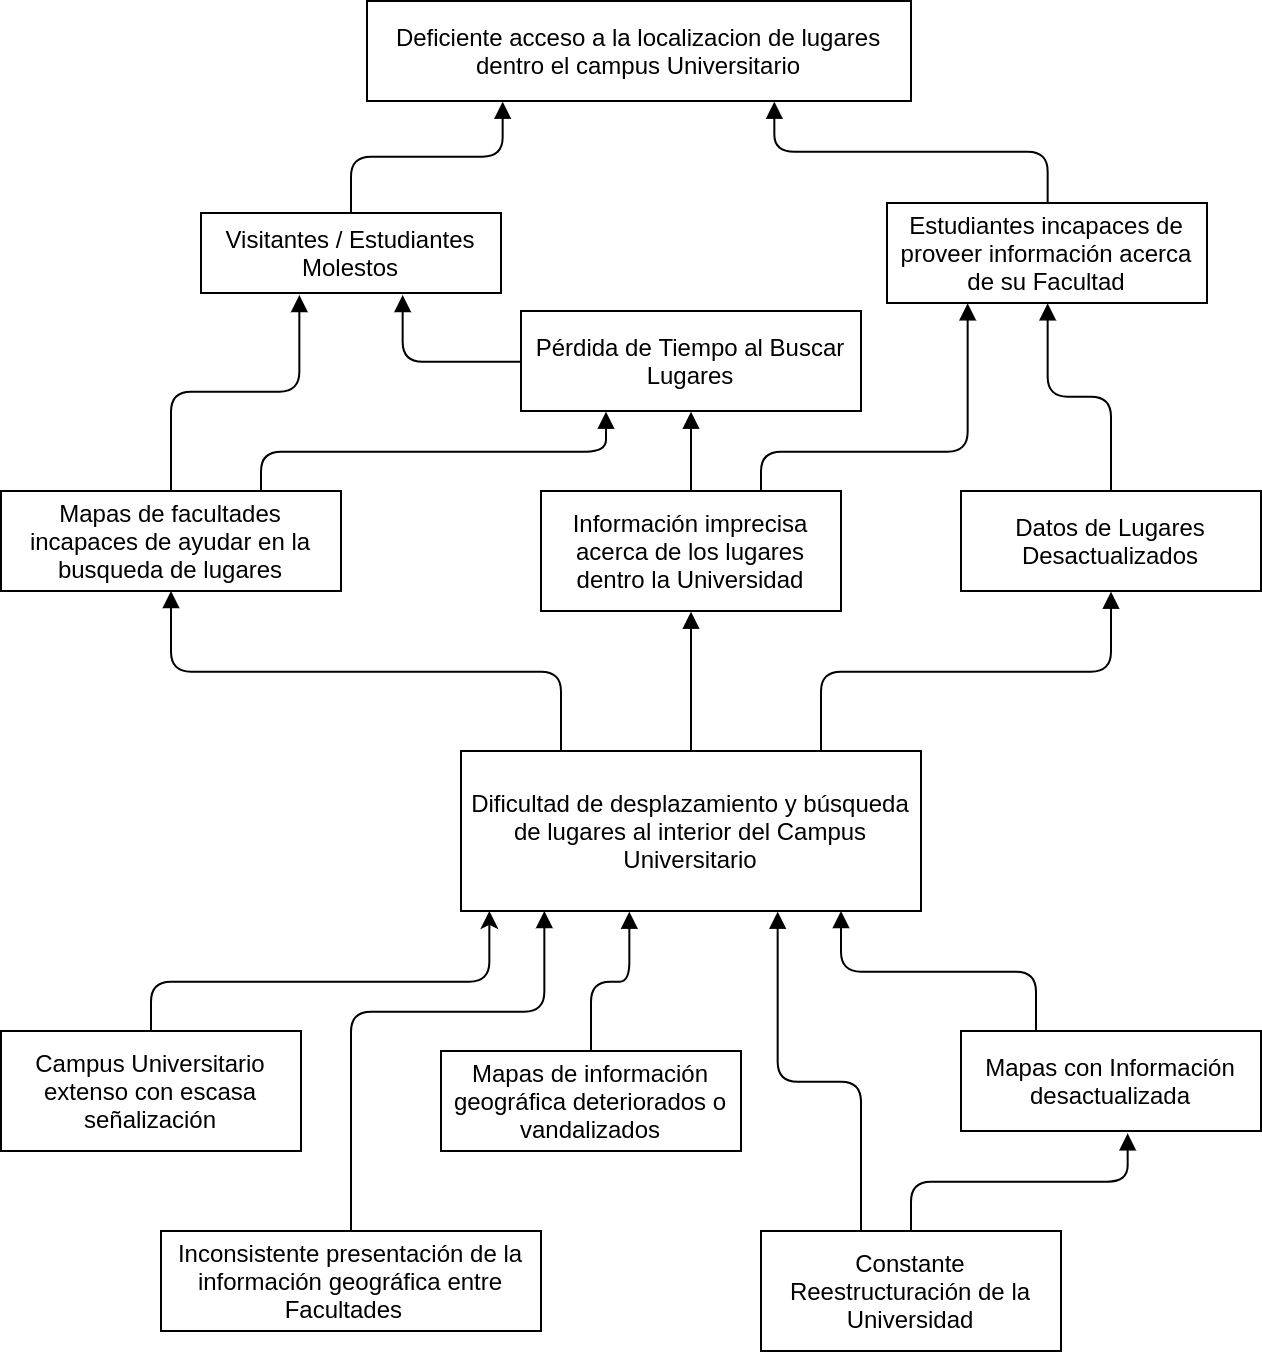
\includegraphics[width=0.65\textwidth]{diagramas/arbolProblemas}
    \end{center}
    \caption{Diagrama Árbol de Problemas}
    \label{fig:arbolProblemas}
    \caption*{Fuente: Elaboración propia}
  \end{figure}

  \section{Objetivo general} % (fold)
  \label{sec:objetivo_general}
    \begin{quote}
      Desarrollar una aplicación web móvil \emph{responsive} para optimizar la búsqueda de lugares y el  desplazamiento al interior del Campus Universitario de la UMSS.
    \end{quote}
  % section objetivo_general (end)


  \section{Objetivos Específicos} % (fold)
  \label{sec:obj_especificos}
    \begin{itemize}
      \item Generar un mapa con información geográfica de las rutas dentro del campus Universitario.
      \item Administrar lugares geolocalizados dentro del campus Universitario.
      \item Mostrar en la aplicación los lugares geolocalizados desplegando la ruta óptima desde mi posición hasta el punto destino.
      \item Administrar usuarios en el sistema.
      \item Registrar las búsquedas sobre rutas realizadas por los usuarios en el sistema.
    \end{itemize}
  % section obj_especificos (end)


  \section{Justificación} % (fold)
  \label{sec:justificacion}

  El Campus Universitario es bastante extenso y se encuentra en constante reestructuración, debido a que las aulas se incrementan, las oficinas son reubicadas, etc. gracias a esto es que los mapas con los que cuenta cada facultad, que son escasos y están impresos sobre banners estáticos, son también difíciles de actualizar. Este hecho genera malestar en estudiantes que llegan tarde a sus clases o necesitan llegar a algún Auditorio o personas/visitantes en proceso de realizar trámites administrativos, no encuentran con facilidad las oficinas a las que necesitan llegar.

  Una aplicación que permita localizar o encontrar locaciones y además proveer la ruta óptima dentro del campus de la Universidad Mayor de San Simón es de gran importancia para brindar apoyo a cualquier persona que necesite desplazarse por el campus Universitario.

  Las Aplicaciones móviles y/o web demostraron ser el futuro del desarrollo de software y la gran mayoría de los países en el mundo consumen estas soluciones y es necesario apuntar a esta tendencia.


  % section justificacion (end)
% chapter introduccion (end)

  \section{Alcance}
  \label{sec:Alcance}

    \subsection{Alcance Práctico}
    \label{sub:alcance_practico}

    Una aplicación web móvil puede llegar a ser muy compleja y manejar información sensible, y ya que el servidor está expuesto al acceso público de los usuarios, es susceptible de ataques maliciosos y malintencionados para acceder y robar información privada que los usuarios podrían tener almacenados en la aplicación, en el caso de la presente aplicación, el sistema no manejará información sensible del usuario, como ser tarjetas de crédito pero la aplicación manejará información de lugares, información que podría ser corrompida por usuarios malintencionados. La seguridad es muy importante para una aplicación web, por lo cual el presente proyecto implementara medidas de seguridad para asegurar la identidad del usuario que está solicitando el ingreso al sistema pero no incluirá protección a ataques Phishing, DoS ya que los objetivos específicos no los contempla.\\


    El \emph{look and feel} de una aplicación web es un tema muy importante para cualquier aplicación a desarrollar, para lograr que la aplicación se muestre de manera consistente en la pantalla de un smartphone se usarán herramientas de terceros pero no se extenderá el uso de la misma para la pantalla de un ordenador de escritorio que posee una resolución de pantalla muy superior al de un celular.\\



    % end alcance_practico

    \subsection{Alcance Metodológico}
    \label{sub:alcance_metodologico}
    Para la conclusión exitosa del presente proyecto se implementará la metodología  Programación Extrema (XP) y cada iteración del proceso tiene como meta el desarrollo conjunto de diferentes módulos, historias de usuario y la documentación relacionada.
    % end alcance_metodologico

    \subsection{Alcance Teórico}
    \label{sub:alcance_teorico}
    La investigación se limita a las estructuras, herramientas y estándares actuales sugeridos en la documentación y bibliografía consultada para la construcción de una aplicación web móvil.
    % end alcance_teorico

  % end Alcance






% Metodología:
% Agile Unified Process (AUP) es una versión simplificada de Rational  Proceso
% Unificado  (RUP).

% Fases del ciclo de desarrollo
%   Principio: El objetivo es  identificar el alcance inicial del proyecto y una
%   arquitectura potencial del sistema.

%   Elaboración: El objetivo es confirmar la idoneidad de la arquitectura del sistema.
%   Construcción: El objetivo es desarrollar software funcional dentro de un sistema regular e incremental periódicamente que mire las necesidades de las partes interesadas.
%   Transición: El objetivo es validar y desplegar el sistema en su entorno de producción.
% Las disciplinas del ciclo de desarrollo se llevan de manera iterativa y son
% las siguientes
%   Modelo: El objetivo de esta disciplina es entender el negocio de la organización, el dominio del problema que se ocupa el proyecto, y determinar una solución viable para hacer frente al dominio del problema.
%   Aplicación: El objetivo de esta disciplina es transformar el modelo de su (s) en el código ejecutable y para llevar a cabo un nivel básico de las pruebas, en las pruebas de unidad en particular.
%   Prueba: El objetivo de esta disciplina consiste en realizar una evaluación objetiva para asegurar la calidad. Esto incluye encontrar defectos, validar que el sistema funcione como está previsto, y verificar que se cumplan los requisitos.
%   Implementación: El objetivo de esta disciplina es el plan para la entrega del sistema y para ejecutar el plan para que el sistema a disposición de los usuarios finales.
%   Gestión de la Configuración: El objetivo de esta disciplina consiste en administrar el acceso a artefactos de su proyecto. Esto incluye no sólo el seguimiento de versiones de los artefactos a través del tiempo, sino también el control y la gestión de los cambios a los mismos.
%   Gestión de Proyectos: El objetivo de esta disciplina es dirigir las actividades que lleva a cabo en el proyecto. Esto incluye la gestión de riesgos, la dirección de personas (la asignación de tareas, seguimiento de los progresos, etc.), y coordinar con la gente y los sistemas fuera del alcance del proyecto para asegurarse de que se entregue a tiempo y dentro del presupuesto.
%   Para el Medio Ambiente: El objetivo de esta disciplina es apoyar el resto de los esfuerzos por garantizar que el proceso, la orientación adecuada (las normas y directrices), y herramientas (hardware, software, etc.) están disponibles para el equipo según sea necesario.
% % Fig. Ciclo de vida del Proceso Unificado Ágil

  %
  \chapter{Marco Teorico} % (fold)
\label{cha:marco_teorico}

La aplicación a desarrollar estará enfocado a su uso en un celular inteligente (smartphone) por lo que hay que determinar el enfoque de desarrollo que se usará y las herramientas necesarias para construir esta aplicación.

\section{Aplicaciones Móviles}
\label{sec:aplicaciones_moviles}

  El desarrollo de aplicaciones web se divide en 3 grupos de enfoques de desarrollo.\\

  \subsection{Aplicaciones Nativas}
  \label{sub:aplicaciones_nativas}

  Las aplicaciones nativas se caracterizan de poder acceder directamente al sistema operativo móvil sin ningún intermediario ni contenedor.\\

  La aplicación nativa puede acceder libremente a todas las APIs (\emph{Application Program Interface} es un conjunto de herramientas, protocolos y rutinas que son usados para desarrollar aplicaciones, un API específica como tienen que interactuar los componentes de un sistema.) que el proveedor del Sistema Operativo (SO) ponga a disposición y, en muchos casos, tiene características y funciones únicas que son típicas del SO móvil en particular.\\

  Este tipo de aplicaciones se adapta al 100\% con las funcionalidades y características del dispositivo obteniendo así una mejor experiencia de uso.\\

  % end aplicaciones_nativas

  \subsection{Aplicaciones Web}
  \label{sub:aplicaciones_web}

  Los dispositivos móviles modernos pueden ejecutar navegadores con capacidad de ejecutar HTML5 (\emph{Hiper Text Markup Language} el cual es el lenguaje para escribir páginas Web), la cual es la Versión de HTML publicado en Octubre 2014, es la más moderna y en la que se escriben todas las aplicaciones web actuales, así como también incorporan un motor JavaScript que permite ejecutar código para lograr una página Web dinámica. Algunos ejemplos del potencial de HTML5 son: componentes IU avanzados, acceso a múltiples tipos de medios, servicios de geoposicionamiento y disponibilidad offline. Al emplear estas características se puede crear aplicaciones avanzadas usando únicamente tecnologías basadas en la Web.\\

  Se debe distinguir entre las aplicaciones Web, las aplicaciones Web diseñadas para dispositivos móviles ya que estas últimas reconocen cuando se accede a través de un smartphone y despliegan una página HTML que fue diseñada para brindar una experiencia táctil y cómoda en una pantalla pequeña, a este diseño de aplicación se le conoce como aplicación web responsive, esto mejora la experiencia del usuario creando un sitio Web móvil que se parezca a una aplicación nativa.\\

  % end aplicaciones_web

  \subsection{Aplicaciones Híbridas}
  \label{sub:aplicaciones_hibridas}

    El enfoque híbrido combina desarrollo nativo con tecnología Web. Usando este enfoque, se escribe gran parte de la aplicación usando tecnologías Web y se mantienen el acceso directo a APIs nativas cuando se necesita. La porción nativa de la aplicación emplea APIs del sistemas operativo para crear un motor de búsqueda HTML incorporado que funciona como un puente entre el navegador y las APIs del dispositivo\cite{IBM_Mobile}.\\

    Esto permite que la aplicación híbrida aproveche todas las características que ofrecen los smartphones modernos. Para lograr esto existen bibliotecas tal como Apache Cordova (antiguamente conocido como \textbf{PhoneGap}, es una de las herramientas más populares para crear aplicaciones híbridas.) que provee una interfaz JavaScript con funcionalidad para conectarse con los dispositivos seleccionados y lograr manejar el API propio del smartphone.\\

    La porción Web de la aplicación puede ser una página Web que resida en un servidor o bien un conjunto de archivos HTML, JavaScript, CSS y contenido multimedia, incorporados en el código de la aplicación y almacenados localmente en el dispositivo\cite{IBM_Mobile}.\\

  % Una mayor fragmentación de dispositivos móviles y tecnologías, lo que, a su vez, va a seguir aumentando los costos generales y las complejidades que conlleva el desarrollo, la integración y la gestión de las aplicaciones móviles

  % end aplicaciones_hibridas

% End aplicaciones_moviles

Para la aplicación se escogió un desarrollo enfocado a tecnología Web diseñado para su uso en smartphones, o una aplicación web responsive. Para lograr este objetivo se usará, tecnologías aplicadas ampliamente en el desarrollo de aplicaciones web.
Para implementar el backend de la aplicación se usará \emph{NodeJS} con \emph{ExpressJS}, la base de datos se construirá sobre \emph{PostgreSQL} y \emph{PostGIS} más \emph{pgRouting}, estos complementos de PostgreSQL nos ayudarán a manejar los datos geoespaciales, para el desarrollo del frontend se usará \emph{EmberJS} y para manejar las imágenes en la web \emph{Cloudinary}.\\

% A continuación se detallara las características y beneficios de cada una de estas herramientas:


\section{Node JS}
\label{sec:node_js}
  Node.js apareció en 2009 y está construido sobre el Motor de JavaScript de Google ``V8'' que fue sacado del browser y aplicado en el servidor.

  Para desarrollar en el lado del browser (cliente) el programador sólo tiene disponible JavaScript como lenguaje de desarrollo pero en el lado del servidor existen muchas alternativas (Ruby, C\#, Python, Java, etc.), JavaScript no estaba disponible.\\

  Node se beneficia del Motor de JavaScript ``V8'' ya que este es rápido y tiene integrado un sistema para manejar las instrucciones de forma asincrónica, pero el mayor beneficio y el porqué Node adquirió una gran popularidad es la facilidad de compartir codigo entre el cliente (browser) y el servidor.\\

  Node.js provee características pero estas pueden parecer complicadas o que necesitan más instrucciones de las necesarias para llevar a cabo acciones que ya son comunes en la creación de aplicación en lado del servidor, por ejemplo a la hora de crear un servidor web, Node se popularizó en gran medida por poder crear servidores web personalizables pero como ya dijimos esto tiene su grado de complejidad, acá es donde entra en acción \emph{Express.js}.


\section{ExpressJS}
\label{sec:express_js}
  \emph{ExpressJS} es un framework que está construido sobre la funcionalidad de servidor web de \emph{NodeJS}, \emph{ExpressJS} ayuda a simplificar el API de Node y añadir nuevas características, diseñadas para mejorar y facilitar la organización de una aplicación \emph{Express}. \cite{understanding_express}\\

  El Cliente (navegador web, aplicación móvil, etc) envía una petición web y el servidor web de \emph{NodeJS} maneja los protocolos web, ley\'endolos y envi\'andolos a una aplicación \emph{ExpressJS} que se encarga de añadir características a la petición y espera la respuesta del ``Middleware Stack'', la función responde a la llamada y el servidor HTTP de Node envía la respuesta mediante los protocolos web al Cliente.\\

  Para escribir un servidor web con \emph{ExpressJS}  no es necesario una gran función para manejar un request, \emph{ExpressJS} contiene utilidades que permite escribir funciones más pequeñas para facilitar el manejo de las peticiones web, haciendo uso de ``middleware'' y ``routing''.

  \subsection{Middleware}
  \label{sub:middleware}
    \emph{NodeJS} maneja una función para trabajar con una petición web, en cambio \emph{ExpressJS} maneja la llamada con varias funciones, cada función se encarga de una pequeña parte del trabajo. Estas pequeñas funciones que manejan la petición web se denominan \emph{Middleware functions} o simplemente \emph{Middleware}.

  %  end sub section middleware

  \subsection{Routing}
  \label{sub:routing}
    Muy parecido al \emph{Middleware}, el \emph{Routing} se encarga de partir una petición web monolítica en pequeñas piezas, pero a diferencia del Middleware, estos manejadores de peticiones se ejecutan condicionalmente dependiendo del URL y la petición HTTP (GET, POST, DELETE) que el cliente envía.\\

  %  end sub section routing

  \emph{ExpressJS} es bastante extensible y cuenta con gran popularidad en la comunidad de desarrollo, la cual provee herramientas para renderizar dinámicamente HTML o interfaces para comunicarse con Bases de Datos, por ejemplo para manejar la conexión y las llamadas a la base de datos PostgreSQL en el presente proyecto se uso la libreria \emph{knex}.


  % \begin{verbatim}
  %   database.any("SELECT * FROM users WHERE id = $1", [userId])
  %     .then(function (data) {
  %         response.send(data.name);
  %     });
  % \end{verbatim}

% section Express JS (end)


\section{Ember JS}
\label{sec:ember_js}

  % Ember is an evolving JavaScript framework for creating “ambitious web applications”, it tries to maximize developers’ productivity using a set of conventions in a way that they don’t need to think about common idioms when building web applications.
  % \vspace*{\fill}
  % \begin{quote}
  % \centering
  % A Framework for creating ambitious web applications
  % \end{quote}
  % % \vspace*{\fill}

Un \emph{framework} o \emph{marco de trabajo} es una abstracción de soluciones a problemas comunes en el desarrollo de software y también provee funcionalidad la cual puede ser modificada por el usuario final, \emph{EmberJS} se define a sí misma como un framework usado para crear aplicaciones web ambiciosas, el cual es eslogan de \emph{EmberJS},con el que trata de decirnos que usando este framework se podría implementar una aplicaciones web con tanta funcionalidad como si se tratara de una aplicación web nativa.\\

Para explicar lo que es EmberJS hay que mencionar que centró su desarrollo en 3 objetivos \cite{ember_antidote}:

\begin{itemize}
  \item Enfocarse en aplicaciones web ambiciosas. %//Focus on ambitious web applications
  \item Previsión de Futuros estándares web. %//Future web standards foresight
  \item Estabilidad sin estancamiento. %//Stability without stagnation []
\end{itemize}

Ember provee una solución completa a los ``problemas'' más comunes en el desarrollo de aplicaciones web, pero esto significa mucho ``más trabajo'' y una curva de aprendizaje más empinada. Pero con una consiguiente ayuda para el desarrollador ya que los ``problemas'' más comunes están resueltos y el desarrollador tiene que enfrentarse a los problemas propios o del modelo de negocio propio de la aplicación a desarrollar.\\

Ember cuenta con su capa de persistencia o la capa del \textbf{Modelo} en el patrón \emph{Modelo-Vista-Controlador}, \emph{Ember-Data}, el cual maneja los datos mientras están en memoria y se asegura de sincronizar con el servidor cuando se requiere y modifica la base de datos. El formato por defecto para manejar la información es \emph{JSON} o \emph{JavaScript Object Notation}, el cual es un formato de texto ligero para el intercambio de datos.\\

% es un patrón de arquitectura de software que separa los datos de una aplicación (Modelo), la interfaz de usuario (Vista), y la lógica de control de la aplicaci\'on (Controlador) en tres componentes distintos\cite{mvc}.

Para facilitar el trabajo de desarrollo en la capa de la \textbf{Vista}, Ember implementa \emph{HTMLHandleBars} el cual es motor de plantillas se usa para separar el diseño HTML de Javascript, para así escribir código mucho más limpio, que permite embeber código enlazando o sincronizado con el Controlador. Esto significa que si actualizamos código en la Vista, este es actualizado en el Controlador y viceversa. [http://handlebarsjs.com/] \\

% \footnote{http://handlebarsjs.com/}

% <Screenshot de uso de HTML HandleBars>

En Ember La capa del \textbf{controlador} es  la encargada de recibir los datos de la Vista y de acuerdo a la interacción del usuario con la aplicación, dispara o activa diferentes acciones que en general modifican los datos ingresados y ya sea para mostrar en UI o guardarlo en la base de datos.\\

% // está siendo deprecada en favor de “Componentes”, esto en favor de la nueva convención “Data down, Actions up”, este cambio es para poder

Ember provee de una herramienta de línea de comandos, \emph{Ember-CLI} o \emph{Ember Command Line Interface}, el cual ofrece para agilizar el desarrollo, usado para automatizar procesos repetitivos, por ejemplo, estableciendo la estructura de directorios del proyecto esto basado en la experiencia de numerosos proyectos, realiza la concatenación, compilación, compresión, y demás manejos de archivos. Como también provee un ecosistema de addons o complementos, que añaden  características nuevas al ecosistema que ofrece \emph{EmberJS}, hay que notar que al ser un proyecto de Software Libre existe una gran cantidad de addons disponibles y cada dia aparecen mas.
Para el desarrollo de este proyecto se hará uso de distintos addons, los cuales se listan a continuación:

\begin{description}
\item[ember-paper:] Este addons es el encargado de adaptar la Vista de la aplicación web en la pantalla de un smartphone, necesario ya que por ejemplo el smartphone no tiene un mouse para hacer click, por el contrario es necesario hacer “tap” con un dedo para ejecutar la misma acción que el mouse, también está el hecho que el tamaño de la pantalla del smartphone es muy inferior a la de un monitor estándar pero la experiencia del usuario tiene que estar diseñada para interactuar con las características que nos ofrece un smartphone.
% <screenshot de la aplicación >

\item[ember-leaflet:] Este addon está diseñado para ayudar a desplegar un mapa, en este caso de estudio se está usando los mapas de OpenStreetMaps™, y optimizado para no usar demasiados recursos, ya que muchas veces los smartphones aún teniendo buenas características no se comparan a una computadora de escritorio.
  % <screenshot de un mapa>

\item[cloudinaryJS:] Addon diseñado para poder manejar las imágenes en la nube, provee varias características como adaptación de la imagen al celular sin hacer uso de nuestro backend o servidor, es de uso libre pero con limitaciones uso en cuanto a las transacciones que se pueden realizar o la cantidad de imágenes que se pueden almacenar.
% <screenshot de imagen>

\end{description}



% end ember_js


  \section{Base de Datos} % (fold)
  \label{sec:base_de_datos}

  En una aplicación web es necesario alguna forma de persistencia de datos, en especial si se están usando datos complejos como la informacion geoespacial, para realizar está tarea, la base de datos es un factor primordial.  Para este proyecto de grado se hara uso de \emph{PostgreSQL} como base de datos relacional y su extension \emph{Postgis} para manejar los datos geoespaciales.\\

    \subsection{PostgreSQL} % (fold)
    \label{sec:postgres}

      PostgreSQL es un sistema de gestión de bases de datos objeto-relacional, Open Source y distribuido bajo licencia BSD.
      PostgreSQL utiliza un modelo cliente/servidor y usa multiprocesos en vez de multihilos para garantizar la estabilidad del sistema. Un fallo en uno de los procesos no afectará el resto y el sistema continuará funcionando.
      La última versi\'on estable de PostgreSQL es la 9.5, su desarrollo comenz\'o hace más de 16 años, y cuenta con una gran comunidad que aporta con el desarrollo y el testeo de nuevas versiones.
      PostgreSQL  está considerada como uno de los mejores \emph{Sistemas de gesti\'on de bases de datos}, es muy completo y está muy bien documentado\footnote{ http://www.postgresql.org/docs/9.5/static/}.
      Entre sus características se pueden nombrar las siguientes.
      \begin{itemize}
        \item Es una base de datos 100\% ACID\footnote{  ACID es un acrónimo de Atomicity, Consistency, Isolation and Durability}
        \item Integridad referencial
        \item Replicación asincrónica/sincrónica
        \item Múltiples métodos de autentificación
        \item Disponible para Linux y UNIX en todas sus variantes
        \item Funciones/procedimientos almacenados
        \item Soporte a la especificaci\'on SQL
      \end{itemize}

      Personalmente se escogió trabajar con  PostgreSQL como DBMS cuenta con una extensa documentación,  y gracias a su caracter ``Open Source'', y su gran flexibilidad en poder definir nuevos tipos de datos, esto se hace posible que empresas como \textbf{Refractions Research}\footnote{http://refractions.net/} puedan crear recursos como \emph{PostGIS}, necesario para trabajar con datos geográficos \'o espaciales.

      % Entre sus principales  características se puede nombrar que es
      % \footnote{ DBMS, DataBase Management System}
      % y durante este tiempo, estabilidad, potencia, robustez, facilidad de administración e implementación de estándares han sido las características que más se han tenido en cuenta durante su desarrollo. PostgreSQL funciona muy bien con grandes cantidades de datos y una alta concurrencia de usuarios accediendo a la vez a el sistema.

    % section postgres (end)

    \subsection{PostGIS} % (fold)
    \label{sec:postgis}

      PostGIS es un módulo  que a\~nade soporte de objetos geográficos al DBMS PostgreSQL, convirtiéndola en una base de datos espacial para su utilización en un Sistema de Informaci\'on Geografica (SIG\footnote{ Es bastante común utilizar el acrónimo en Inglés, Geographic Information System (GIS), de hay viene el término de PostGIS = Postgres + GIS}).

      El desarrollo de PostGIS está a cargo de Refractions Research, está liberada con la \emph{Licencia pública general de GNU}, declarandola como software libre que lo protege de cualquier intento de apropiaci\'on.\\

      PostGIS implementa la especificaci\'on ``SFSQL'' (Simple Features for SQL, define los tipos y funciones que necesita implementar cualquier base de datos espacial) de la \emph{OGC} (Open Geospatial Consortium, es un consorcio internacional, formado por un conjunto de empresas, agencias gubernamentales y universidades, dedicado a desarrollar especificaciones de interfaces para promover y facilitar el uso global de la información espacial).\\

      \emph{PostGIS} al igual que \emph{PostgreSQL} cuenta con una documentaci\'on bastante extensa y equipo de desarrollo que continuamente va sacando nuevas versiones, actualmente se encuentra la versi\'on 2.2.2, pero para el desarrollo de la aplicaci\'on se hizo uso de la versi\'on 2.1.0.

      PostGIS es gratis, pero no por ello es una herramienta de baja calidad, al contrario se la considera una herramienta de nivel empresarial, y muchas instituciones la est\'an usando de manera exitosa\footnote{ http://www.postgis.org/documentation/casestudies/}, aparte de numerosas aplicaciones.\\

      Manejar los datos geográficos con PostGIS es sencillo y eficiente, por está raz\'on se utilizó está herramienta, pero para conseguir la ruta óptima entre 2 puntos se necesitaba el uso del algoritmo de Dijkstra y para PostGIS existe el módulo \textbf{PgRouting}, que tiene implementado este algoritmo.

      \subsubsection{pgRouting} % (fold)
      \label{sec:pgrouting}
        pgRouting es una extensi\'on  de  PostGIS para proveer funcionalidades de ruteo espacial. pgRouting es un desarrollo posterior de pgDijkstra y actualmente está siendo mantenido por Georepublic, la última versi\'on estable es la 2.1, y es la que fue usada para desarrollar el sistema.\\

        Las ventajas del ruteo en la base de datos son:
        \begin{itemize}
          \item Los datos y atributos pueden ser modificados desde varios clientes, como \emph{Quantum GIS} y \emph{uDig} a través de \emph{JDBC}, \emph{ODBC}, o directamente usando \emph{Pl/pgSQL}. Los clientes pueden ser PCs o dispositivos móviles.
          \item Los cambios pueden ser reflejados instantáneamente a través del motor de ruteo. No hay necesidad de hacer cálculos previos.
          \item El parámetro de ``costo'' puede ser calculado dinámicamente a través de SQL y su valor puede provenir de múltiples campos y tablas.
        \end{itemize}

        pgRouting provee funciones para:
        \begin{itemize}
          \item Camino mínimo (Dijkstra): algoritmo de ruteo sin heurística
          \item Camino mínimo (A-Star): routeo para conjunto de datos grandes (con heurística)
          \item Camino mínimo (Shooting-Star): ruteo con restricciones de giro (con heurística)
          \item El problema del viajante (TSP: Traveling Salesperon Problem)
          \item Cálculo de ruta (Isolíneas)
        \end{itemize}

        % Uses PostGIS for its geographic data format, which in turn uses OGC’s data format Well Konwn Text (WKT) and Well Known Binary (WKB)
      % section pgrouting (end)
    % section postgis (end)
  % section base_de_datos (end)


  \section{Metodologia de Desarrollo}
  \label{sec:metodologia_de_desarrollo}
    La metodologia para el desarrollo de software nos permite gestionar y administrar un proyecto de desarrollo de software para llevarlo a termino de una forma mas eficiente y con altas probabilidades de exito.\\
    Seguir una metodología es importante ya que nos ayudara a organizarnos y a seguir un ritmo de trabajo.\\
    Para este proyecto de grado se hará uso de una metodología Ágil. Para lo cual se definirá en que se basan las metodologías ágiles.\\

    Para este proyecto de grado se va a ser uso de \emph{XP} como metodologia agil.\\

    \subsection{Metodologías \'Agiles}
    \label{sub:metodologias_agiles}

    Este término nace en una reunión celebrada en febrero de 2001 en Utah - USA por expertos en la industria del software ya que pretendían encontrar una forma alternativa de desarrollo de software a las que estaban vigentes hasta esa fecha por ejemplo la metodología en cascada que es rígido y obliga una planeación extensiva antes siquiera de tocar una línea de código, esta demostrado que este tipo de metodologías son muy rígidas y les falta flexibilidad a la hora de hacer frente a los cambios que invariablemente sufre un proyecto de desarrollo de software.\\

    % //·        In reality it is very difficult for projects to follow the sequential flow of the model
    % //·        It is difficult to identify all requirements and goals at the beginning of projects as requirements tend to change all the way
    % //·        A working version can only be obtained late in the process


    Para contravenir estas dificultades es que se definieron los principios de manifiesto ágil:

    \begin{quote}
      \begin{description}
        \item[Individuos e interacciones] sobre procesos y herramientas
        \item[Software funcionando] sobre documentación extensiva
        \item[Colaboración con el cliente] sobre negociación contractual
        \item[Respuesta ante el cambio] sobre seguir un plan
      \end{description}
    \end{quote}

    % The main concern of agile methodologies is the ability to embrace changes which are very likely to happen in environments which lack predictability [6]

    El principal objectivo de las metodologías ágiles es la habilidad de soportar los cambios, los cuales generalmente por no decir casi siempre aparecen en un ambiente que sufre muchos cambios y rápidamente, los cuales son difíciles de predecir.\cite{6}\\

    % //To achieve the objective, agile methodologies use three key principles [8]: (1) a focus on adaptive methodologies, (2) a focus on people, and (3) a focus on self-adaptive processes.

    Para alcanzar este objetivo es que las metodologías ágiles se basan en tres principios\cite{8}:

\begin{itemize}
  \item Enfoque en metodologías que se adapten al cambio
  \item Enfocarse en las personas
  \item Enfocarse en procesos que se auto-adapten al cambio
\end{itemize}

    Las metodologías ágiles no se refieren a un único y específico metodo o tecnica de desarrollo, en cambio son un grupo de metodologías que implementan los principios ágiles. Entre los cuales se pueden apreciar las siguiente metodologías:\\

    \begin{itemize}
      \item Scrum
      \item Dynamic Systems Development Method (DSDM)
      \item Crystal Methods
      \item Feature Driven Development
      \item Lean Development
      \item Extreme Programming (XP)
      \item Adaptive Software Development
    \end{itemize}


    Por las siguientes caracteristicas de la Metodologia \emph{Programaci\'on extrema}, la cual viene del ingles \emph{eXtreme Programing} por lo cual generalmente nos referiremos a esta como \emph{XP} es que es la escogio para implementar este proyecto de grado.


    % End metodologias_agiles


    \subsection{Programaci\'on Extrema}
    \label{sub:xp}

      Programaci\'on extrema o \emph{XP} es una metodología de trabajo creada a mediados de 1990 por Kent Beck cuando estaba trabajando en un proyecto de desarrollo de software en Chrysler Comprehensive Compensation (C3)\cite{KhenBeck} en un intento de mejorar el proceso de desarrollo de software y posteriormente con una segunta implementación de un proyecto usando la metodologia XP en \emph{Vehicle Cost and Profitability System (VCAPS)} en \textbf{Ford Motor Co}\cite{KhenBeck} se demostró que esta metodología de desarrollo es un método apropidado para llevar a buen termino el proyecto de desarrollo.\\

      \emph{XP} se enfoca en la adaptabilidad ya que el desarrollo de software debería ser un proceso fluido donde los requerimientos no pueden ser totalmente predichos desde el principio del desarrollo ya que estos siempre o casi siempre tienden a cambiar a medida que el software se va desarrollando ya sea por cambios en el mercado o a medida que el cliente va aprendiendo y modificando sus requerimientos en el transcurso del ciclo de desarrollo del producto.\\

      Kent Beck encontró que cuatro enunciados las cuales son la base de la filosofía de XP\cite{KhenBeck}:\\

      \begin{itemize}
        \item Es necesario mejorar la comunicación
        \item Es necesario encontrar simplicidad
        \item Es necesario obtener feedback o retroalimentación de parte del cliente
        \item Es necesario proceder con coraje.
      \end{itemize}

      Combinando estos principios, la programación extrema se trata acerca de mejorar el trabajo en equipo cohesionadolo y con la ayuda de la retroalimentación propia del equipo se puede apreciar donde se encuentra y mejorarlo, siempre tomando en cuenta que cada equipo es único, ya sea por el tipo de software que se está desarrollando y por las personas que conforman el equipo.\\

      Las prácticas usadas en XP son de hecho prácticas comúnmente usadas en las metodologías ágiles pero en XP estas prácticas son llevadas al extremo de ahí el nombre de programacion extrema.\\

      La programación extrema se caracteriza por las siguiente practicas:

      \begin{description}
        \item[Code reviews:] O revisión de código, en programación extrema esto se llama programación en pareja (pair programing), esto significa que dos programadores escriben código usando o compartiendo una máquina, esto se traduce en que el código es constantemente revisado y por lo tanto es menos proclive de producir errores.

        \item[Testeo:] en XP significa hacer unit testing o pruebas unitarias durante todo el proceso de desarrollo de software, una vez el producto es entregado al cliente este se encarga de probar la funcionalidad del sistema.

        \item[Diseño:] en XP se necesita que todos los involucrados en el proyecto estén siempre y constantemente refactorizando y mejorando el producto.
        Simplicidad: Siempre dejar el sistema con el diseño más simple posible para que soporte la funcionalidad deseada o lo más simple que funciona. Se basa en la filosofía de que el mayor valor de negocio es entregado por el programa más sencillo que cumpla los requerimientos.

        \item[Arquitectura:] Todos trabajando definiendo y redefiniendo constantemente la arquitectura del sistema.
        Testeo de integración: Unir o integrar y probar las diferentes características del software que se están trabajando, constantemente o por lo menos una vez al dia.

        \item[Iteraciones cortas:]
        Trabajar en ciclos realmente cortos, puede ser de horas o días pero no semanas o meses, permitiendo que el programa, el verdadero valor del negocio, pueda ser evaluado.

        \item[Propiedad colectiva del código:]
        un código con propiedad compartida. Nadie es el propietario de nada, todos son el propietario de todo. Este método difiere en mucho a los métodos tradicionales en los que un simple programador posee un conjunto de código.


        \item[Estándar de codificación:] define la propiedad del código compartido así como las reglas para escribir y documentar el código y la comunicación entre diferentes piezas de código desarrolladas por diferentes equipos

        \item[Bienestar del programador:] La semana de 40 horas, la programación extrema sostiene que los programadores cansados escriben código de menor cualidad. Minimizar las horas extras y mantener los programadores frescos, generará código de mayor calidad.

      \end{description}


      \subsubsection{Las historias de usuario}
      \label{subs:user_story}


      Es la técnica que utiliza XP para especificar los requisitos del software. Se trata de tarjetas en las cuales el cliente escribe las características que el sistema debe poseer, sean requisitos funcionales o no funcionales. El proceso de manejar las historias de usuario es muy dinámico ya que se pueden añadir, eliminar o modificarse de acuerdo a la exigencia que puede aparecer a cualquier momento, las historias deben ser lo bastante simples como para que los programadores las implementen en unas semanas.\cite{xpesp}
      % end user_story

      \subsubsection{Proceso de desarrollo}
      \label{subs:proceso_desarollo}

      La programación extrema identifica las siguientes fases en el proceso de desarrollo de software

      \begin{description}
        \item[Interacción con el cliente:]
        El cliente es una parte importante en el equipo de desarrollo, tiene gran importancia en el equipo ya que expresa su opinión sobre el producto después de cada cambio o iteración, mostrando las prioridades y expresando su opinión sobre los problemas que se podrían identificar.

        \item[Planificación del proyecto:]
        En este punto se se elabora la planificación por etapas o iteraciones. Para hacerlo será necesaria la existencia de reglas que han de seguir las partes implicadas en el proyecto.

        \item[Diseño, desarrollo y pruebas:]
        El desarrollo es la parte más importante en el proceso de la programación extrema. Todos los trabajos tienen como objetivo que se programen lo más rápidamente posible, sin interrupciones y en la dirección correcta.\cite{xpesp}

      \end{description}


      %end proceso_desarollo


      \subsubsection{Roles de la programación extrema}
      \label{subs:roles_xp}

      \begin{description}
        \item[Programador:] Escribe las pruebas unitarias y produce el código del sistema.
        \item[Cliente:] Escribe las historias de usuario y las pruebas funcionales para validar su implementación. Asigna la prioridad a las historias de usuario y decide cuáles se implementan en cada iteración centrándose en aportar el mayor valor de negocio.
        \item[Tester:] Ayuda al cliente a escribir las pruebas funcionales. Ejecuta pruebas regularmente, difunde los resultados en el equipo y es responsable de las herramientas de soporte para pruebas.
        \item[Tracker:] Es el encargado de seguimiento. Proporciona realimentación al equipo. Debe verificar el grado de acierto entre las estimaciones realizadas y el tiempo real dedicado, comunicando los resultados para mejorar futuras estimaciones.
        \item[Entrenador (coach):] Responsable del proceso global. Guía a los miembros del equipo para seguir el proceso correctamente.
        \item[Consultor:] Es un miembro externo del equipo con un conocimiento específico en algún tema necesario para el proyecto. Ayuda al equipo a resolver un problema específico.
        \item[Gestor (Big boss):] Es el dueño de la tienda y el vínculo entre clientes y programadores. Su labor esencial es la coordinación.\cite{xpcyta}
      \end{description}


      % end roles_xp

      \section{Desarrollo del Proyecto usando XP} % (fold)
      \label{sec:desarrollo}

      Ya que para el desarrollo del proyecto se usará programación extrema,
      se va a definir el proceso de desarrollo general que se usará en este proyecto de grado.\\

        % \section{Proceso de Desarrollo}
        % \label{sec:proceso_de_desarrollo}

        XP propone un proceso iterativo e incremental, El proyecto es dividido en pequeños “mini-proyectos”, los cuales terminan con un release\footnote{\emph{Release} es una versión del producto que se libera al final de un ciclo de desarrollo de software, un release contiene requerimientos implementados, tal vez no acabados en un  100\% pero funcional de tal forma el cliente es capaz de ofrecer feedback del producto.} o lanzamiento.\\

      En un proyecto que sigue la metodología XP los releases son frecuentes, esto para recibir feedback más seguido. Los releases son negociados en un Planning Game, donde los clientes definen qué se va a implementar en el release y los desarrolladores especifican el tiempo que necesitan para desarrollar las características deseadas.\\

      \begin{figure}[H]
        \caption{Diagrama del proceso XP}
        \label{fig:xp_diagram}
        \begin{center}
          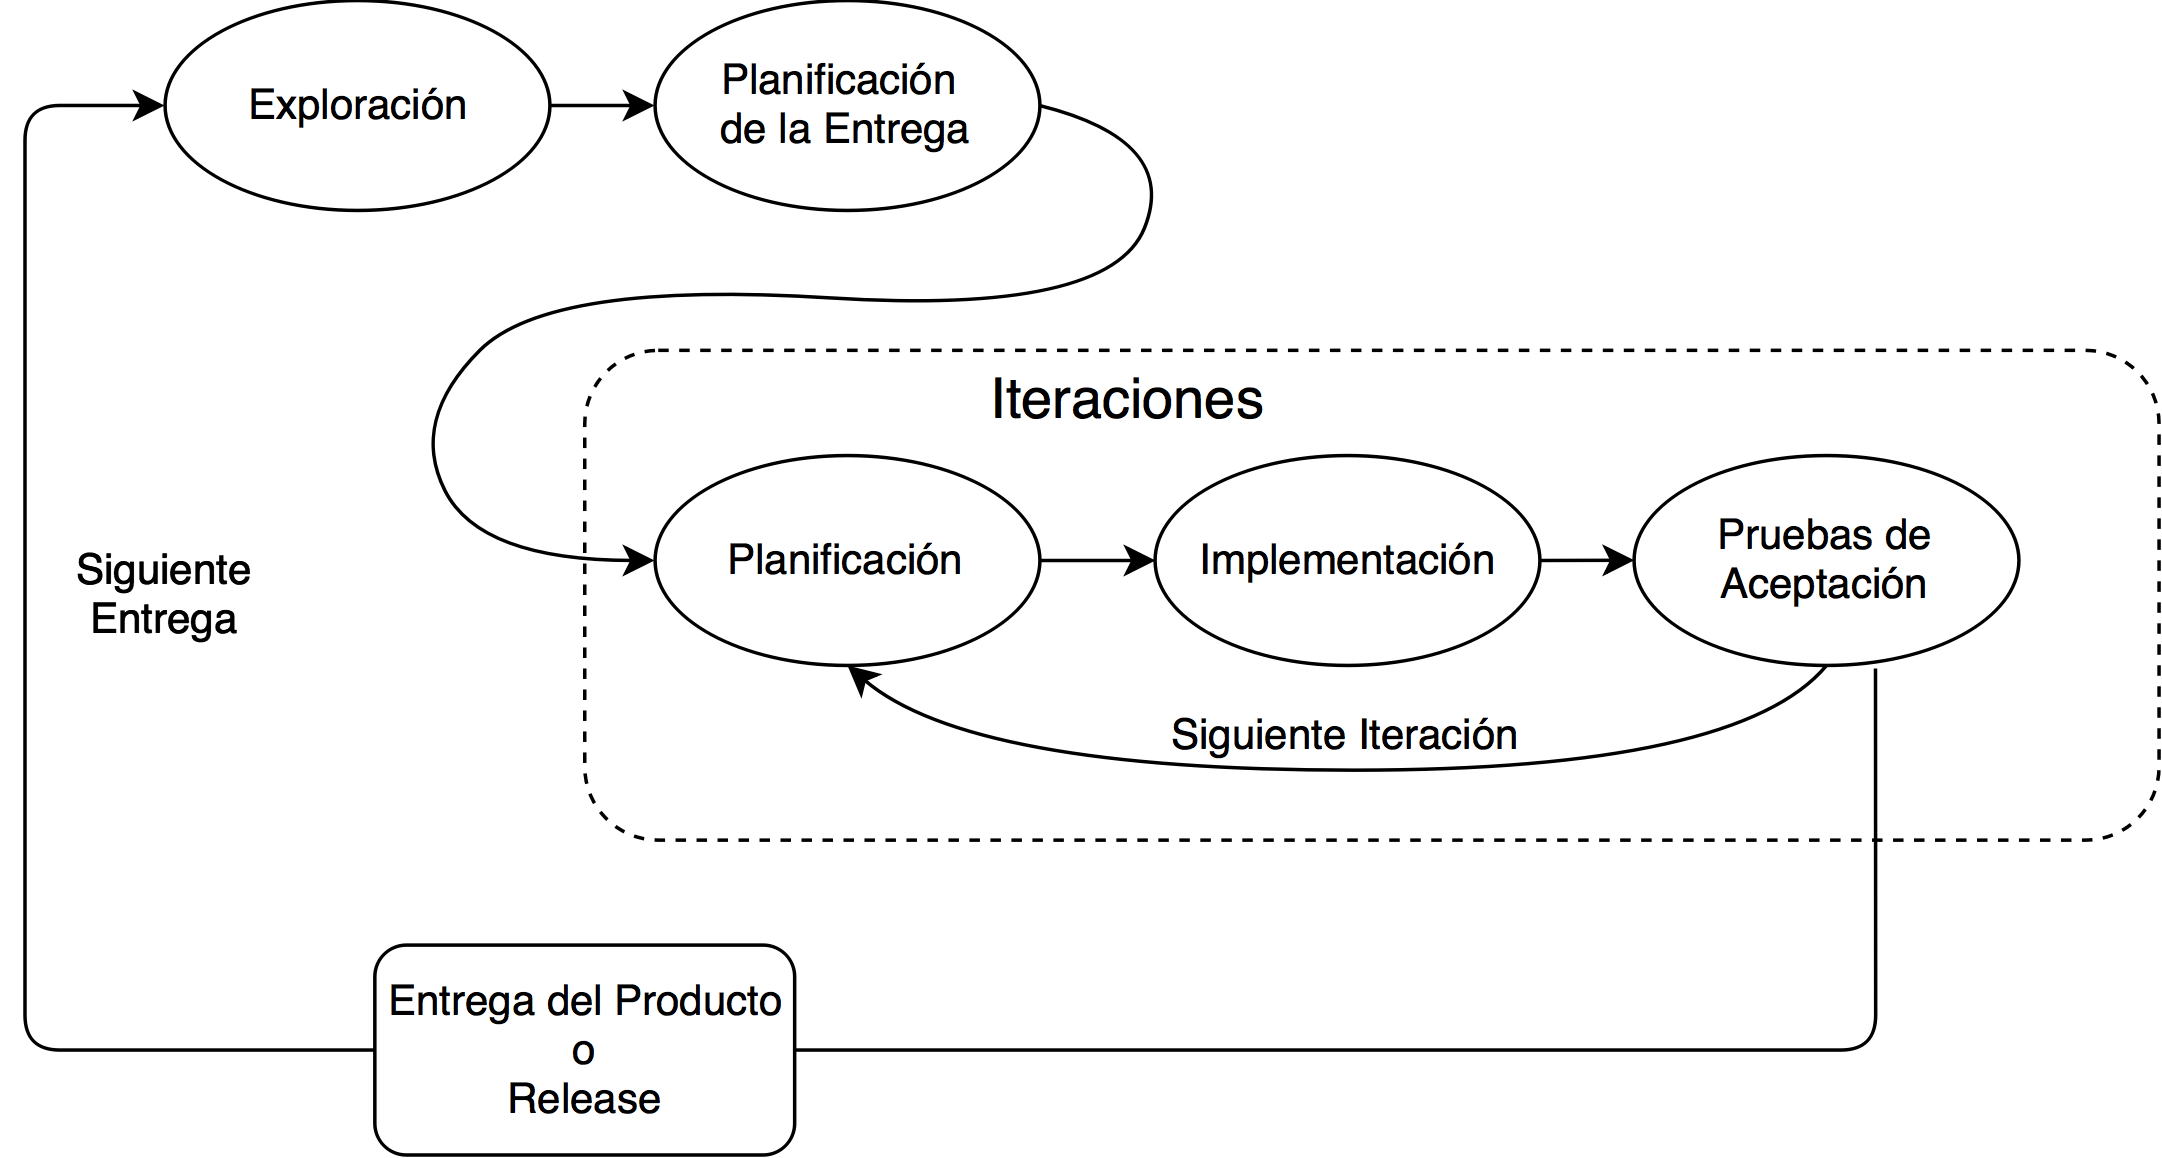
\includegraphics[width=1\textwidth]{xp_diagram}
        \end{center}
        \caption*{Fuente: Elaboración propia}
      \end{figure}

      En la figura \ref{fig:xp_diagram} se puede apreciar el proceso de desarrollo de la metodología XP, la cual se explicará a continuación.\\

        \subsection{Planning Game}
        \label{sub:planning_game}

        La fase del planning game consiste de 3 etapas: exploración, planeaci\'on y direcci\'on.\\

        Durante la fase de la \textbf{exploración} los clientes definen lo que desean que tenga el sistema y los desarrolladores estiman el tiempo necesario que necesitan para realizar esas tareas.\\

        Durante la \textbf{planeación} se negocia y se decide cuales de todas las características que los clientes quieren pueden llegar a realizarse en el tiempo dise~ado para una iteración.\\

        Después de la planeación sigue la fase de \textbf{dirección}, durante la cual se desarrolla y actualiza (cuando sea necesario) la planeación ya negociada según lo que se vaya aprendiendo a medida que avanza el desarrollo del proyecto.\\

          \subsubsection{Exploración}
          \label{subs:exploracion}
            Durante esta etapa el cliente escribe las tarjetas de historias de usuario, estas historias definen lo que el cliente quiere que el sistema haga, en otras palabras representan las características que el sistema debería tener implementado.\\

            Una vez que estas tarjetas están escritas, el equipo de desarrollo debe asignarles una estimación en términos del tiempo necesitado para el desarrollo y el riesgo para el producto que pueden llegar a tener las características detalladas en las historias del usuario.\\

            Las historias del usuario se las crea para propósitos de planeación y estimación de tiempo y esfuerzo que cada característica va a necesitar, los detalles se crean y dividen posteriormente cuando las historias están por ser implementadas en las “tareas de ingeniería”.\\
          % end exploracion

          \subsubsection{Planeación}
          \label{subs:planeacion}

            Cuando se tienen las historias del usuario junto con las estimaciones de los desarrolladores, se está listo para una “negociación de aceptación” donde un “calendario de entregas”  es negociado y donde se aceptan qué historias se van a desarrollar primero en cuanto tiempo se van a entregar resultados.\\

          % end planeacion

          \subsubsection{Dirección o Steering}
          \label{subs:steering}

          Esta fase es básicamente comprende el resto del desarrollo del producto hasta que es liberado al mercado o el proyecto es cancelado.\\

          Esta fase consiste en 4 ``movimientos'':

          \begin{description}
            \item[Iteración:] Es durante la iteración cuando se desarrolla el producto, el tiempo que se utiliza para esta fase es de generalmente de una o 2 semanas, dependiendo de la naturaleza del proyecto.

            \item[Recuperación:] Si durante el desarrollo no se completan las características a desarrollar en el tiempo establecido, es durante la recuperación que se re-negocia con el cliente si quiere cambiar la fecha de entrega del release o modificar el alcance del desarrollo (menos historias de usuario).

            \item[Nuevas Historias:] El cliente tiene el derecho de aumentar historias de usuario, las cuales se tienen que estimar y negociar si serán parte del actual desarrollo, en tal caso se tiene que renegociar las fechas de entrega.

            \item[Re-estimación:] Si durante el desarrollo el equipo considera que el plan ya no es correcto, todas las historias que faltan hacer se tienen que re-estimar y el plan se tiene que re-negociar con el cliente.
          \end{description}

        % end planning_game

          \subsection{Iteration Planning Game}
          \label{sub:iteracion}

            % \subsubsection{Iteración}
            % \label{subs:iteracion}

            La fase de Iteración en XP se lo denomina como Iteration Planning Game, esta al igual que  el release planning game consiste en las fases de: Exploración, Planning e Implementaci\'on. Steering.\\

            Hay que tomar en cuenta que la planeación de una iteración en particular es desarrollada al inicio de cada interacción, no se planifican iteraciones por adelantado.\\

            Generalmente cada 3 iteraciones se actualiza el Calendario de Entregas “committed schedule” para reflejar los logros alcanzados por el equipo de desarrollo y el estado del proyecto, también sirve para identificar posibles riesgos.\\

            \subsubsection{Exploración}
            \label{subs:exploracion}

            Durante esta fase el cliente escoge las historias de usuario que serán implementadas en la presente iteración, generalmente se escogen las que aportan más valor al producto o tienen más relevancia en la lógica de negocio del cliente, asi como tambien cualquier historia que no se acabó en una iteración anterior.\\

            Los desarrolladores dividen las historias en Tareas de Ingeniería, las cuales son más pequeñas que las historias, si se encuentra que una Tarea es casi tan grande como una historia es porque es una historia y debería ser dividida en Tareas. Una tarea puede estar relacionada a 2 o mas historias o no estar relacionada con ninguna historia. Dentro de la metodología XP es una buena práctica el escribir las tareas en las  “Index Cards”, similares a las historias, esto debido a que estas tarjetas son fáciles de manipular durante la fase de planeación.\\

            % end exploracion

            \subsubsection{Planeación}
            \label{subs:planeacion}

            Durante esta fase un desarrollador acepta la responsabilidad de implementar una Tarea de acuerdo de su experiencia personal en el área y tecnologías que se usarán en el desarrollo. El desarrollador debe estimar el tiempo necesitado para completar la tarea en un \emph{Ideal Engineering Time} Tiempo de Ingenieria Ideal, siempre hay que considerar que la tarea se deriva de la Historia de usuario que es escogido para la iteración actual, una regla de XP consiste en que no se debe realizar trabajo el cual no se va necesitar ahora, \textbf{YAGNI}\footnote{You aren't gonna need it. En espa\~nol, Tu no lo vas a necesitar \'o No vas a necesitarlo.}.\\

            La Tarea combinada con el nombre del desarrollador responsable, la estimación asignada son parte del \emph{Iteration Schedule} \'o \emph{Plan de la Iteración}, con el cual el equipo de desarrollo es capaz de determinar si la iteración está \emph{floja} o \emph{cargada}, si está \emph{floja} se pueden añadir otras historias a la iteración o si está \emph{cargada} es necesario dividir historias.\\
            Finalmente cuando la carga de trabajo de la iteración está balanceada se procede con la siguiente fase, la \emph{Implementación} de las tareas.


            % end planeacion

            \subsubsection{Implementación}
            \label{subs:implementacion}

            % dentro de la Implementación una Tarea de desarrollar.
            Dentro de lo que es el ciclo de desarrollo de software, \textbf{XP} define el siguiente procedimiento:

            \begin{itemize}
              \item Analizar lo que hay que hacer, esto envuelve lo que es analizar las Tarjetas de Ingeniería y/o las historias de usuario. %, de ser necesario se realiza una sesión CRC.
              \item Escribir Pruebas Unitarias, son bastante útiles para determinar cuando la tarea está completada.
              \item Implementar el código suficiente para lograr que las pruebas unitarias pasen exitosamente.
              \item Simplificar el código si es necesario (Refactor Mercilessly).
              \item Integrar los cambios continuamente (Continuous Integration).
            \end{itemize}
            % end implementacion

            \subsubsection{Registrar el Avance}
            \label{subs:registrar_avance}
            XP define un rol en específico que se encarga de medir el progreso, el Tracker.

            \subsubsection{Verificación}
            \label{subs:verificacion}
            Cada historia lleva asociado test funcionales, que están diseñados para verificar que los criterios de aceptación de cada historia están implementados. \\
            Si durante esta fase las pruebas fallan, la historia de usuario relacionada se marca para volver a trabajar en ella en la siguiente iteración.\\


            % end iteracion

          % end steering



        % end proceso_de_desarrollo
    % end xp


  %
  %
  % Para el presente proyecto de grado se implementará los siguientes roles:
  % Programador, Cliente, Tester, roles que serán representados por mi persona.
  % Tracker y entrenador será representado por el Tutor.
  % Consultor será representado por la docente de proyecto final


  % end metodologia_de_desarrollo

\chapter{Geolocalización} % (fold)
\label{cha:geolocalizacion}

  La Geolocalización o Georreferenciación es un término bastante nuevo, de hecho no aparece en el diccionario de la Real Academia Española, no obstante se lo puede definir como:
% \footnote{http://dle.rae.es/}

  \begin{quote}
    El posicionamiento en el que se define la localización de un objeto espacial (representado mediante un punto, vector, área, volumen) en un sistema de coordenadas y datum determinado. Este proceso es utilizado frecuentemente en los Sistemas de Información Geográfica.\cite{Georreferenciacion}
  \end{quote}

  % Para entender esta definición se necesita explicar algunos términos

  La Georreferenciación antiguamente era bastantemente usada en el ámbito científico, y se necesitaba de instrumental y personal cualificado para su manejo, pero en la actualidad la cantidad de dispositivos con capacidad para geolocalizar un objeto sobre la tierra es bastante común, de hecho todos los smartphones actuales (en general los que se consideran gama media o alta) traen integrados receptores GPS (Global Position System), y sumados a la explosión de aplicaciones  que integran mapas con localización, ya que se puede tener una base de datos con coordenadas, descripciones, etc., que individualmente no aporta mucho valor pero al obtener datos de una gran cantidad de usuarios puede llegar a ser informacion valiosa ya que sirve para tomar decisiones a nivel de negocio, pero interpretar estos datos sería muy difícil sin la ayuda de los \emph{Sistemas de Información Geográfica} o \emph{SIG}.\\

  Un SIG es una herramienta que permite integrar, analizar, mostrar, interpretar y  entender las relaciones, patrones y tendencias de la información geográficamente referenciada \cite{what_is_gis}.
  % \footnote{http://www.esri.com/what-is-gis}
  Por estas razones es que actualmente existe una explosión de estas aplicaciones, donde empresas, particulares y hasta organismos gubernamentales están haciendo uso de estas tecnologías.
  Y las posibilidades son diversas, por ejemplo, si se quisiera planificar la construcción de un colegio se podría integrar los datos del censo con un mapa, identificando los sectores con mayor porcentaje de niños y localizando los sectores más propicios para realizar la construcción del inmueble. En el caso de una catástrofe natural, el tener las rutas de evacuación geolocalizadas y disponibles en un mapa de manera eficiente,  ayudaría en la evacuación de las personas del lugar.\\

  La geolocalización es actualmente una tecnología y una herramienta usada en gran medida por una gran cantidad de aplicaciones web, añadiendo búsquedas y resultados personalizados a nivel país, ciudad, barrio y calle, resultando en una gran variedad de servicios y que actualmente es de gran ayuda en diferentes escenarios. La geolocalización ayuda a moverse por una ciudad, encontrar restaurantes, cines, transporte, etc. actualmente es una de las herramientas mas usadas y desarrolladas a nivel de industria, comercio, turismo, etc. y vale la pena estudiarla y entenderla.\\



  \section{Definiciones} % (fold)
  \label{sec:definiciones}

    En la aplicación desarrollada se requerirá trabajar con datos espaciales, y para ello es necesario entender algunos conceptos envueltos en el manejo de la información geográfica.

    \begin{description}
      \item[Coordenada:] Es una secuencia de n-números que designa la posición de un punto en un espacio n-dimensional.
      \item[Sistema de coordenadas:] Un sistema de coordenadas es  un conjunto de reglas matemáticas que especifican cómo las coordenadas son asignadas  a cada  punto.
      \item[Punto:] Es  la representación de una posición, topológicamente 0-dimensional (no tiene volumen, área, longitud o cualquier otra unidad multi-dimensional).
    \end{description}

    % \section{Coordenada} % (fold)
    % \label{sec:coordenada}
    %   Es una secuencia de n-números que designa la posición de un punto en un espacio n-dimensional. \\
    %   % one of a sequence of n-numbers designating the position of a point (4.17) in n-dimensional space
    %   % NOTA: En un
    %   % NOTE In a coordinate reference system, the numbers shall be qualified by units.

    % % subsection coordenada (end)

    % \section{Sistema de coordenadas} % (fold)
    % \label{sec:sistema_de_coordenadas}
    %   Un sistema de coordenadas es  un conjunto de reglas matemáticas que especifican cómo las coordenadas son asignadas  a cada  punto.
    %   % set of mathematical rules for specifying how coordinates (4.3) are to be assigned to each point (4.17)

    % % subsubsection sistema_de_coordenadas (end)
    % \section{Punto} % (fold)
    % \label{sec:punto}
    %   Es  la representación de una posición, topológicamente 0-dimensional (no tiene volumen, área, longitud o cualquier otra unidad multi-dimensional).
    %   % topological 0-dimensional geometric primitive (4.15), representing a position
    % % subsection punto (end)

    Estas definiciones están desarrolladas en la especificación \emph{Simple Feature Access}, la cual es mantenida por la OGC (Open Geospatial Consortium). Esta especificación define el conjunto de tipos de datos (puntos, línea, polígono, etc) y las operaciones o métodos necesarios para manejar estos datos.

    % \footnote{\url{http://www.opengeospatial.org/standards/sfa}}

  % section definiciones (end)
  \section{Sistema de Coordenadas para datos Geográficos} % (fold)
  \label{sec:sistema_de_coordenadas_para_datos_geograficos}
    Se podría pensar en un sistema de coordenadas como la forma de dar sentido a un \emph{par de coordenadas}, por ejemplo \verb|POINT(-66.1457475 -17.3937285)|, cómo se interpretan estos números?.
    Podría ser la latitud y longitud del campus de la UMSS, o algun punto en el Oceano Pacifico. Es gracias al sistema de coordenadas que se puede ubicar este punto en el Universo.\\


    Una aplicación que maneja datos geográficos tiene que trabajar con sistemas de coordenadas relacionadas con la superficie terrestre, conocidas como coordenadas espaciales o coordenadas globales, que permiten representar la tierra en \emph{3-Dimensiones} (3D), ya que esta es una Esfera, mas especificamente un esferoide oblato\footnote{Un \emph{esferoide oblato} (o elipsoide oblato) es un elipsoide de revolución obtenido por rotación de una elipse alrededor de su eje más corto.}, o en una representación de la superficie terrestre en \emph{2-Dimensiones} (2D), los sistemas de coordenadas se clasifican en: Coordenadas geocéntricas, Coordenadas Geográficas y Coordenadas Proyectadas.

    \subsection{Coordenadas geocéntricas (X,Y,Z)} % (fold)
      \label{sub:coordenadas_geocentricas}
        También conocido como \emph{Coordenadas Cartesianas 3D}, Este sistema tiene como origen el centro de la Tierra, con el \emph{eje X} y el \emph{eje Y} en el plano del ecuador. El \emph{eje X} pasa a través del meridiano de Greenwich, y el \emph{eje Z}  coincide con el eje de rotación de la Tierra. como se puede ver en la figura \ref{fig:coord_geocentric}.

        \begin{figure}[H]
          \begin{center}
            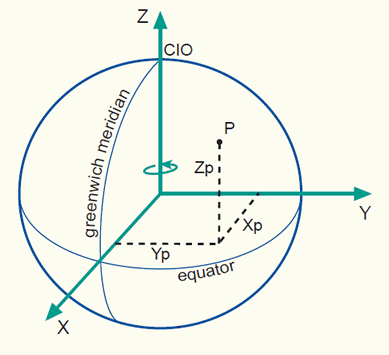
\includegraphics[width=0.7\textwidth]{coord_geocentric}
            \caption{Sistema de coordenadas Geocéntricas}
            \label{fig:coord_geocentric}
            \caption*{Fuente: \cite{coords2009} }
          \end{center}
        \end{figure}

        Este sistema de coordenadas no es muy usado en la representación de datos, pero a veces se lo requiere para análisis de algoritmos y geometría computacional.
      % subsection coordenadas_geocentricas (end)

      \subsection{Coordenadas Geográficas} % (fold)
      \label{sub:coordenadas_geograficas}
        El sistema de coordenadas Geográficas, ver figura \ref{fig:coord_geographic}, utiliza las coordenadas angulares latitud  (\emph{phi} o ${\phi}$) y longitud (\emph{lambda} o ${\lambda}$). Este sistema de coordenadas se expresa en grados, se lo puede representar con la forma \emph{grados:minutos:segundos }\verb|(17° 23' 37.4226" S, 66° 8' 44.691" W)|, o de la forma más común \emph{grados decimales} \verb|(-66.1457475 S, -17.3937285 W)|. \\

  Dentro de ese sistema de coordendas, esta el que es el más ampliamente usado y el que usan por defecto los sistemas \emph{GPS}, es el denominado ``WGS 84'' (\emph{World Geodetic System 1984}) y es el que generalmente la mayoría de las aplicaciones usan para el manejo de mapas. Es el sistema que maneja los más ampliamente conocidos ``latitud y longitud''.\\

        \begin{figure}[H]
          \begin{center}
            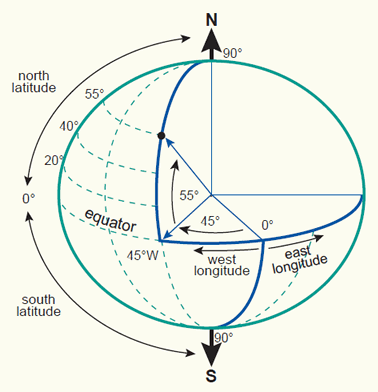
\includegraphics[width=0.7\textwidth]{coord_geographic}
            \caption{Sistema de coordenadas Geográficos}
            \label{fig:coord_geographic}
            \caption*{Fuente: \cite{coords2009} }
          \end{center}
        \end{figure}




      % subsection coordenadas_geograficas (end)

      \subsection{Coordenadas Proyectadas} % (fold)
      \label{sub:coordenadas_proyectadas}
        Un sistema de coordenadas proyectadas es una representación plana y bidimensional de la  tierra. Se basa en un sistema de coordenadas \emph{geográficas esféricas}, pero utiliza unidades de \emph{medida lineales} para las coordenadas, de forma que los cálculos de distancia y área se pueden realizar en términos de esas mismas unidades. \cite{projected}

        Un sistema de coordenadas proyectadas requiere tomar la superficie esférica de la tierra y ``aplanarla'', este procedimiento se lo realiza con la finalidad de tener un mapa representable en una hoja de papel así como en la pantalla de la computadora. Sin embargo este procedimiento introduce diversos tipos de distorsión por lo que existen diferentes clases de proyecciones que varían según la región de la Tierra que se quiere representar.

        La proyección que usan por ejemplo, \emph{Google Maps} y \emph{Open Street Maps} es la \emph{Mercator Projection}, esta proyección está diseñada para preservar los ángulos y las formas de las líneas en forma recta, pero distorsiona los tamaños y las distancias mientras más lejos se encuentran de la línea del Ecuador. Esta proyección se puede apreciar en la figura \ref{fig:mercator_proyection}. \cite{gmaps_osm}

% Google Maps usa la Proyección de Mercator para mostrar su mapa

        \begin{figure}[H]
          \begin{center}
            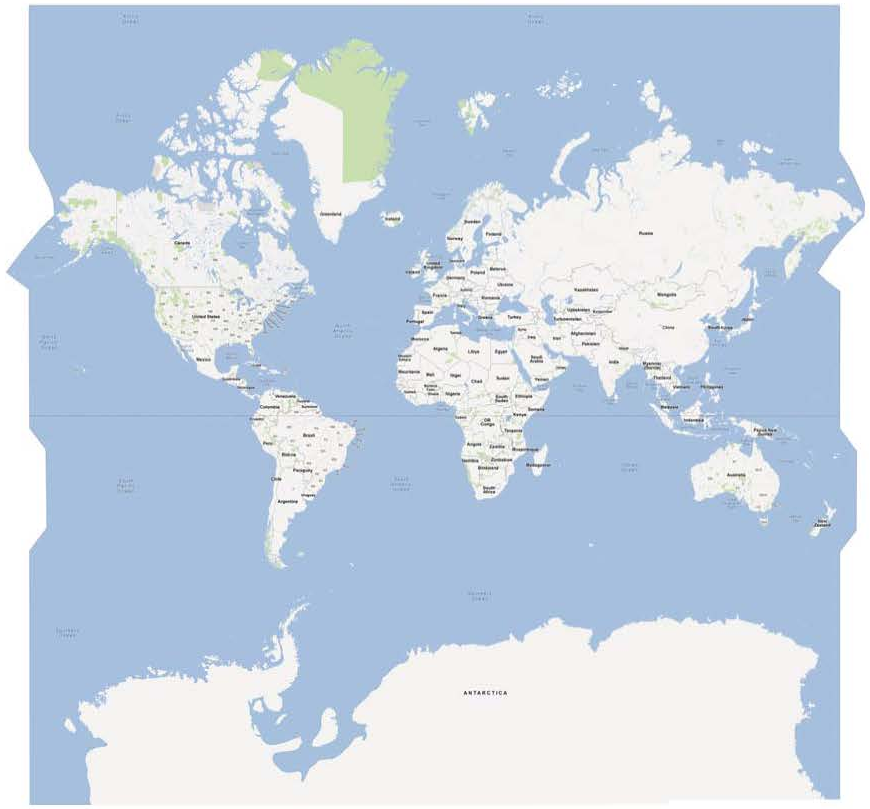
\includegraphics[width=0.6\textwidth]{mercator_proyection}
          \end{center}
          \caption{Sistema de coordenadas Proyectadas}
          \label{fig:mercator_proyection}
          \caption*{Fuente: \cite{coords2009} }
        \end{figure}

        Tal como se puede apreciar en la figura \ref{fig:mercator_proyection}, la distorsión de esta proyección se hace evidente si se observa la zona de Groenlandia ya que parecería tan grande como África o América del Sur, cosa que no es cierta, ya que Groenlandia es casi 14 veces más pequeño que África. A pesar de esta distorsión tan marcada, la \emph{Proyección de Mercator} es una de las más usadas.
         % de hecho Google Maps usa esta proyección.
      % subsection coordenadas_proyectadas (end)

  %
  %     \section{Que se usó en la Aplicación} % (fold)
  %     \label{sec:que_se_uso_en_la_aplicacion}
  %       Es importante entender las diferencias entre los distintos tipos de sistemas de coordenadas porque computacionalmente realizar operaciones sobre los sistemas de coordenadas tiene un costo.
  %       Si se usara el sistema de coordenadas geográfico (WSG84) este es el más apropiado si se necesitaría usar grandes extensiones de la superficie terrestre, que al ser una estructura elipsoidal el costo computacional para realizar las operaciones matemáticas de calcular distancias, intersecciones, etc. es más elevado. En cambio el uso de un sistema de coordenadas proyectado (Mercator Projection) tiene un costo computacional más bajo, ya que se estaría trabajando con un sistema geométrico.\\
  %
  %       % Por otro lado,
  %       También hay tomar en cuenta la base de datos, ya que será esta la que se encargará de manejar los datos espaciales. Al estar usando PostGIS, se puede ver que en su documentacion\footnote{ http://postgis.org/documentation/manual-1.5/ch04.html} que claramente exorta el uso de un sistema geometrico sobre el uso de un sistema geografico si  se va trabajar con datos que cubran una pequena area geografica. Tomando en cuenta esta recomendación y el tamaño del área de estudio (el campus de la UMSS), se procedió a implementar en la base de datos el uso de la proyección Mercator. Se va usar Mercator sobre las otras proyecciones porque aparte de las ventajas que se mencionaron con anterioridad, Google Maps usa esta proyección y ya que se usará este mapa lo más correcto es trabajar con la misma proyección.
  %
  %
  %       % Comoprojected
  %       % PostGIS maneja dos tipos de datos, geográficos y geométricos
  %
  %     % section que_se_uso_en_la_aplicacion (end)
  % % section sistema_de_coordenadas_para_datos_geograficos (end)
  % % \section{Tipo de archivos} % (fold)
  % % \label{sec:tipo_de_archivos}
  % %
  % % section tipo_de_archivos (end)
  %
  % \section{Implementación} % (fold)
  % \label{sec:Implementacion}
  %   Para manejar datos georreferenciados con tecnología JavaScript, ya que se implementó el Backend con NodeJS, se hizo uso de la librería \textbf{KnexJS} para manejar la conexión a la base de datos PostgreSQL, y BookshelfJS para las consultas SQL pero para las consultas con datos geospaciales se realizó a través de esta herramienta pero usando la forma \emph{Raw SQL}\footnote{Raw SQL se refiere a consultas en ``SQL puro'' ya que el fuerte de BookshelfJS es el manejo de las consultas en forma de objetos (ORM), lamentablemente actualmente no existe mucho soporte para manejar datos geoespaciales}.
  %
  %   \begin{center}
  %     \begin{verbatim}
  %       var raw = "SELECT " +
  %                   " ST_AsGeoJSON(geom)::json As geometry," +
  %                   " name," +
  %                   " description," +
  %                   " phone," +
  %                   " level," +
  %                   " gid As id " +
  %                 " FROM place WHERE LOWER(name)
  %                        like LOWER('%" + name + "%')";
  %     \end{verbatim}
  %   \end{center}
  %
  %   De esta forma es que se recupera de la base de datos un lugar georreferenciado, donde este tiene un nombre, una descripción, un teléfono, el nivel o piso donde se encuentra pero lo importante de esta consulta es la obtención del ``punto'' geoespacial del lugar.
  %
  %   \begin{center}
  %     \begin{verbatim}
  %       "POINT (-66.14857015827988 -17.394421906929086)"
  %     \end{verbatim}
  %   \end{center}
  %
  %   % var raw = "SELECT seq, id1 AS node, id2 AS edge, cost
  %   %            FROM pgr_dijkstra('SELECT gid AS id,
  %   %                                     source::integer,
  %   %                                     target::integer,
  %   %                                     st_length(geom) AS cost
  %   %                               FROM public.ways', targetId, sourceId, false, false);";
  %
  %
  %    Este atributo es de tipo \emph{punto} o \emph{point} el cual tiene un \emph{SRID}\footnote{ Spatial Reference System Identifier, El \emph{SRID} corresponde a un sistema de referencia espacial basado en el elipsoide concreto usado para la creación de mapas de tierra plana o de tierra redonda.\cite{msdn_srid} } \emph{3857}\footnote{La proyección Mercator usa el EPSG 3857}, el SRID  es la llave primaria de la tabla \emph{spatial\_ref\_sys} que se crea cuando se inicializa una base de datos que soporte informacion geoespacial (PostGis), esta tabla provee la información necesaria para interpretar y convertir correctamente todas las coordenadas existentes, el \emph{SRID 3857} está definida en la tabla \emph{spatial\_ref\_sys} como ``Popular Visualisation CRS / Mercator''.\\
  %
  %
  %   Obtener la coordenada es el primer paso, seguidamente se debe mostrarlo sobre un mapa, en este caso \emph{Open Street Maps}, como se puede apreciar en la figura \ref{fig:ember_leaflet}, esta interfaz está implementada usando \emph{ember-leaflet}, el cual está principalmente diseñada para ofrecer una mejor experiencia de usuario en celulares smartphones.\\
  %
  %   % \begin{center}
  %   %   \begin{verbatim}
  %   %     var maker = new google.maps.Marker({
  %   %       position: new google.maps.LatLng( lat, lng  )
  %   %       map: UMSS.map
  %   %     });
  %   %   \end{verbatim}
  %   % \end{center}
  %
  %   \begin{verbatim}
  %     {{#leaflet-map lat=lat lng=lng zoom=zoom}}
  %       {{tile-layer url="http://{s}.tile.openstreetmap.fr/hot/{z}/{x}/{y}.png" }}
  %         {{#marker-layer location=location}}
  %           <h3>{{model.name}}</h3>
  %           {{model.description}} <br>
  %           <strong>telf:</strong> {{model.phone}} <br>
  %           <strong>piso </strong>#{{model.level}}
  %       {{/marker-layer}}
  %     {{/leaflet-map}}
  %   \end{verbatim}
  %
  %   \begin{figure}[H]
  %         \begin{center}
  %           \caption{\emph{ember-leaflet} nos ayuda a desplegar un mapa y mostrar un \emph{punto} o \emph{lugar} con un \emph{marcador} y dibuja una línea de color rojo sobre el mapa.}
  %           \label{fig:ember_leaflet}
  %           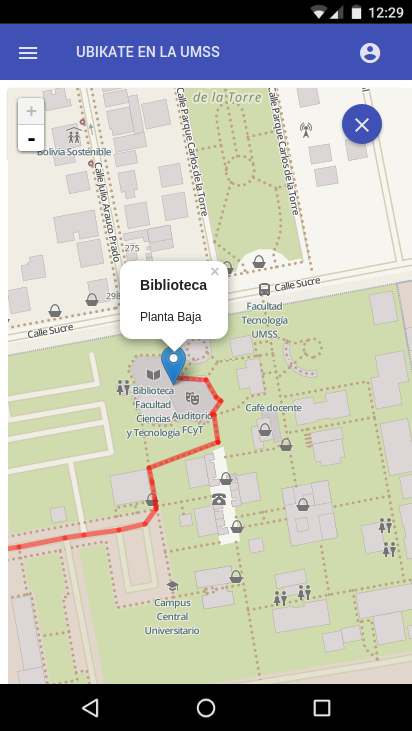
\includegraphics[width=0.5\textwidth]{ember_leaflet}
  %         \end{center}
  %         \caption*{Fuente: Elaboración propia.}
  %   \end{figure}
  %
  %

    % Pero esta coordenada  no sería  fácil de entender sin una adecuada representación sobre un mapa,


  % section Implementacion (end)
  % \section{Los datos} % (fold)
  % \label{sec:los_datos}


  %   Una vez implementada la Base de datos es necesario insertar ``los datos''
  % % section los_datos (end)


  % -------------------------------------------------------------------
  % -------------------------------------------------------------------
% -------------------------------------------------------------------

  % \section{Conclusión} % (fold)
  % \label{sec:geo_conclusion}
  %
    %
    % Los Mapas son herramientas muy útiles a la hora de desplegar información, pero realizar el mapa, crear las fórmulas matemáticas con las cuales se trabajará, determinar cómo se usarán estas fórmulas para una representación adecuada de la superficie terrestre, es una tarea muy compleja. Como programador la tarea más complicada fue determinar el tipo de mapa y el sistema de coordenadas más adecuado para el tipo proyecto que se necesita desarrollar.\\
    %
    % Los términos de longitud y latitud son en un inicio, más fácilmente comprendidos que un sistema proyectado, pero no se puede tomar a la ligera una correcta comprensión del uso de los \emph{sistemas de coordenadas} en una base de datos espacial, un mal uso de estos conceptos puede generar errores a la hora de manejar datos  espaciales o en el resultado de las operaciones sobre estos  datos, llegando a resultados no deseados y que pueden costar más tiempo y dinero en una posterior corrección.\\
    %
    %
    % Para dibujar líneas rectas sobre un mapa hay que tomar en consideración que la tierra no es plana y las líneas que en un mapa parecen líneas rectas, realmente no son rectas, ya que el planeta Tierra es un \emph{esferoide oblato} por lo que las líneas en apariencia rectas tienen la curvatura natural del planeta Tierra. En distancias largas se nota mucho mas la utilidad de usar mapas con \emph{sistemas proyectados}, pero también es cierto que para una área pequeña como es el campus de la Universidad de San Simón este problema no tiene un gran impacto pero no está demás en tomar en cuenta esta característica en el análisis de datos geoespaciales, tomando en cuenta estas caracteristacas de la Geolocalizacion se llego a la conclucion de usar
    % el sistema de \emph{coordenadas projectadas}, mas especificamente la proyección \emph{SRID 3857}.\\
    %
    %
    %
    % La geolocalización es actualmente una tecnología y una herramienta usada en gran medida por una gran cantidad de aplicaciones web, añadiendo búsquedas y resultados personalizados a nivel país, ciudad, barrio y calle, resultando en una gran variedad de servicios y que actualmente es de gran ayuda en diferentes escenarios. La geolocalización ayuda a moverse por una ciudad, encontrar restaurantes, cines, transporte, etc. actualmente es una de las herramientas mas usadas y desarrolladas a nivel de industria, comercio, turismo, etc. y vale la pena estudiarla y entenderla.\\
    %
    %
    %





% ************************************************************
    % Maps are deceivingly simple tools, and cartography a surprisingly complex discipline. While the most trouble many of us will have with a map is figuring out how to fold it, this simplicity belies great sophistication that has been developed over the years.
  % section geo_conclusion (end)


  % \begin{description}
  %   % \item[SIG] Un Sistema de Información Geográfica es una manera de visualizar como es y que está ocurriendo en algún lugar. La posibilidad de incorporar coordenadas con precisión.

  %   % A GIS is a collection of software, normally manipulated by its user through a single interface, and designed to perform a wide range of operations on geographic data.
  %   % Research  Methods in Geography
  %   % Basil Gomez and John Paul Jones III.
  %   % ISBN 978-1-4051-0710-5

  %   \item[Datum]
  %   \item[]
  %   \item[]
  % \end{description}

  % procesar
  % Se tien
  % , Sistema de Posicionamiento Global por sus siglas en espanol
% chapter geolocalizacion (end)

\section{Ruta Óptima} % (fold)
\label{cha:ruta_optima}

En general el mejor camino o el más óptimo para ir de un punto a otro es aquel que toma menos tiempo en ser recorrido, pero para definir que un camino es óptimo hay que tomar en cuenta las características de este, por ejemplo, si se va en coche hay que tomar en cuenta la dirección de las calles, los cruces, etc. si se va caminando hay que ver las características del terreno, caminos cortados, distancias, etc.\\


Encontrar la ruta óptima entre 2 puntos es un problema al cual se enfrentan las personas diariamente, por ejemplo, las empresas de transporte, de correo, etc., necesitan mejorar la eficiencia del trayecto y a la vez reducir el consumo de combustible, para mejorar la atención al cliente y a la vez reducir costos de operación. \\

Dentro el campus Universitario es generalmente prioritario optimizar el tiempo de busqueda de algun lugar o punto de interés al cual se quiera llegar, ya sea como estudiante o visitante externo.\\


Si se analiza el terreno que se va a cubrir con la aplicación, el campus ``Las Cuadras'' de la Universidad Mayor de San Simón ubicado entre las calles Oquendo, Sucre,  Belzu y M. U. López, se tiene que el camino óptimo es siempre el más corto o de menor longitud, el método de desplazamiento que se tomara en cuenta será \emph{caminando}, el terreno es llano y la única restricción es respetar las rutas peatonales.\\

% El problema de la ruta más corta es ampliamente usado por las empresas de transporte, correos, etc., que necesitan mejorar la eficiencia del trayecto y a la vez reducir el consumo de combustible, dentro del campus universitario, reducir el tiempo en el cual encontramos un aula o una oficina mejoraría en gran medida la presentación de la Universidad hacia gente externa que necesitan hacer uso o encontrar algún lugar en especifico ya que lamentablemente esta información actualmente sólo te la pueden ofrecer las personas que conocen el lugar de antemano y aun en esos casos existe la posibilidad de no encontrar el lugar que se está buscando.\\
% La resolución de este problema es la se analizará en este capítulo.

El presente problema se lo podría definir como, encontrar la ruta más corta de un punto a otro punto, donde los puntos están interconectados por una red de caminos. El problema descrito se lo puede resolver y describir como un caso específico de la teoría de grafos.



  \subsection{Grafos} % (fold)
  \label{sec:teoria_grafos}


    % \section{Definiciones} % (fold)
    % \label{sec:grafos_definiciones}
      Inicialmente es necesario aclararar algunos términos usados en la teoría de grafos.

      % El grafo que es la reprentacion

      % \begin{description}
      %   \item[Grafo] Un grafo G consiste en un conjunto  vértices V y un conjunto de aristas A, y se lo escribe como G(V,E).
      %   \item[Vertice]
      % \end{description}

      \begin{itemize}
        \item \textbf{Grafo:} Un \emph{grafo} $G$ consiste en un conjunto de vértices $V$ y un conjunto de aristas $A$, y se lo representa con $G(V,A)$.

        \item  \textbf{Vértice:} El \emph{vértice} \emph{v} es adyacente a \emph{u}, o a un vecino de \emph{u}, si y sólo si $(u,v) \in A$. Los vértices también son llamados nodos.

        \item  \textbf{Arista:}
        Cada \emph{arista} o arco es representada por un par de elementos $(u,v)$, donde los elementos $u,v \in V$, son los nodos que une la arista.

        % Para fines prácticos, no  consideraremos las aristas de la forma (u,u)

        \item \textbf{Grafo no Dirigido:}
        En un \emph{grafo no dirigido} $G$, dos vértices $u$ y $v$ se dice que están conectados si hay un camino en $G$ de $u$ a $v$ (y cómo $G$ no es dirigido, también hay un camino de $v$ a $u$). Un grafo  se denomina completo si para todos los pares $u,v \in V$ existe una arista $(u,v) \in A$.

        % En un \emph{grafo no dirigido}, dado una arista $(u,v)$, $v$ es adyacente de $u$, y simétricamente \emph{u} es adyacente de \emph{v} y si el par de vértices que representan la arista no tiene orden, por lo tanto la arista $(u,v)$ y $(v,u)$ representa la misma arista.

        \item \textbf{Grafo Dirigido:} En cambio en un \emph{grafo dirigido} las aristas $(u,v)$ y $(v,u)$ representan dos diferentes aristas. También se puede anotar un tercer componente, llamado peso o costo, en ese caso estaríamos hablando de un \emph{grafo ponderado}.

        % Un camino en un grafo es una secuencia de nodos $v_{1}$, $v_{2}$, \ldots{}, $v_n$ tal que $(v_{1}, v_{2}), (v_{2}, v_{3}), \ldots{}, (v_{n-1}, v_n)$ son aristas.
        %
      \end{itemize}



    % \end{description}
    % subsection grafos_definiciones (end)
    % \subsection{Representacion de un Grafo} % (fold)
    % \label{sec:representacion_de_un_grafo}
      Existen diversas formas de representar un grafo sea dirigido o no-dirigido, pero entre las mas usadas están la matriz de adyacencias y la lista de adyacencias.

      \subsection{Matriz de adyacencias de un Grafo} % (fold)
      \label{sub:matriz_de_adyacencias_de_un_grafo}
        Sea $G = (V,A)$ un grafo de \emph{n} vértices. La matriz de adyacencias $M$  para $G$ es una matriz $M_{nxn}$ de valores booleanos, donde $M(i,j)$ es verdad si y sólo si existe un arco desde el nodo \emph{i} al nodo \emph{j}.

        \begin{displaymath}
          M(i,j) = \left\{
          \begin{array}{ l l }
            1, & \textrm{si existe la arista } (i,j) \\
            0, & \textrm{en caso contrario}
          \end{array} \right.
        \end{displaymath}


        Las filas y las columnas de la matriz representan los nodos del grafo.
        Cuando el grafo es no-dirigido la matriz de adyacencias es simétrica, como se puede ver en el grafo de la figura \ref{fig:grafo_ponderado} y su correspondiente matriz de adyacencias.
        % El cuadro \ref{tab:matriz} representa la matriz de adyacencias de la figura \ref{fig:grafo_ponderado} representa
        % La matriz de adyacencias, que se puede observar a continuacion, es la  misma matriz de la relación $A$ de $V$ en $V$ porque indica cuales vertices están relacionados o unidos por una arista.


        % \begin{tikzpicture}[->,>=stealth',shorten >=1pt,auto,node distance=3cm,
        %         main node/.style={circle,draw,font=\sffamily\Large\bfseries}]
% !ht
        \begin{figure}[H]
          \begin{center}

            \begin{tikzpicture}[->,>=stealth',shorten>=1pt,auto,node distance=3cm,main node/.style={circle,draw,font=\sffamily\Large\bfseries}]

              \node[main node] (1) {a};
              \node[main node] (2) [below right  of=1] {b};
              \node[main node] (3) [above right of=2] {c};
              \node[main node] (4) [below left of=2] {d};
              \node[main node] (5) [right of=2] {e};
              % \node[main node] (6) [right of=5] {f};
              % \node[main node] (7) [above right of=6] {g};
              % \node[main node] (4) [below right of=1] {d};

              \path[every node/.style={font=\sffamily\small}]
                (1) edge node [auto] {3} (2)
                    edge node[left] {5} (4)
                (2) edge node[left] {8} (3)
                    edge node[right] {4} (4)
                    edge node[auto] {3} (5)
                (3) edge node[left] {7} (5)
                (4) edge node[below] {14} (5);

            \end{tikzpicture}

            \caption{Grafo ponderado no-dirigido}
            \label{fig:grafo_ponderado}
            \caption*{Fuente: Elaboración propia}

          \end{center}
        \end{figure}

        % La matriz de adyacencias, que se puede observar a continuacion, es la  misma matriz de la relación $A$ de $V$ en $V$ porque indica cuales vertices están relacionados o unidos por una arista.


        \begin{table}[H]
          % \label{tab:matriz}
          \begin{center}
            \begin{displaymath}
              M(i,j) =
              \bordermatrix{ ~ & a & b & c & d & e \cr
                             a & 0 & 3 & 0 & 5 & 0 \cr
                             b & 3 & 0 & 8 & 4 & 3 \cr
                             c & 0 & 8 & 0 & 0 & 7 \cr
                             d & 5 & 4 & 0 & 0 & 14\cr
                             e & 0 & 3 & 7 & 14& 0  }
            \end{displaymath}
            \caption*{Matriz de adyacencias del grafo de la figura  \ref{fig:grafo_ponderado}}
          \end{center}
        \end{table}


      % subsubsection matriz_de_adyacencias_de_un_grafo (end)

    % subsection representacion_de_un_grafo (end)
    \subsection{El Problema de la ruta mas corta} % (fold)
    \label{sec:ruta_mas_corta}
      Dados los vértices $v_{i}$ y $v_{j}$ de un grafo $G = (V,A)$ se llama trayectoria mínima o camino minimo  de \(v_i\) a \(v_j\) al numero de aristas del camino de longitud mínima que va desde $v_i$ a $v_j$ y se representa por $d(v_i, v_j)$.

      Cuando en el grafo no exista un camino de $v_i$ a $v_j$ se dice que el camino minimo es $d(v_i, v_j) = \infty$ \\

      Para determinar el camino mínimo que va desde un único vértice a cualquier otro vértice se puede usar el algoritmo de Dijkstra.



      \subsubsection{Algoritmo de Dijkstra} % (fold)
      \label{sub:algoritmo_de_dijkstra}
      El algoritmo de  Dijkstra fue descrito en 1959 por \emph{Edsger Dijkstra}, y permite encontrar la trayectoria más corta entre dos nodos específicos, cuando los valores de los arcos son todos positivos\\

      El algoritmo asigna un etiqueta a cada nodo en el grafo. Esta etiqueta es la distancia que hay desde el nodo \emph{s} escogido como origen a lo largo de la trayectoria más corta encontrada, hasta el nodo que se está etiquetando.\\

      La etiqueta de cada nodo puede estar en 2 estados:

      \begin{itemize}
        \item[\textbf{a.}] Puede ser permanente; en este caso la distancia encontrada es a lo largo de la trayectoria, la más corta de todas las encontradas.
        \item[\textbf{b.}] Puede ser temporal; cuando hay incertidumbre de que la trayectoria encontrada sea la más corta de todas.
      \end{itemize}

      A medida que el método trabaja se cambian gradualmente las etiquetas temporales por etiquetas permanentes. Al comienzo se tiene un conjunto de nodos con etiquetas temporales y el objetivo es hacer que esas etiquetas disminuyan, encontrando trayectorias a esos nodos usando trayectorias a nodos etiquetados permanentemente. Cuando esto se ha logrado, se selecciona el nodo con la etiqueta temporal más pequeña y esta etiqueta se convierte en permanente. El proceso se repite hasta que al nodo terminal \emph{t} se le haya asignado una etiqueta permanente, pero esto puede ocurrir eventualmente, ya que cada vez que el algoritmo es usado, una de las etiquetas es omitida y así el número de nodos con etiquetas temporales decrece a cero. \cite{teoria_grafos} \\


      % subsection algoritmo_de_dijkstra (end)
    % subsection ruta_mas_corta (end)
  % section teoria_grafos (end)


% ********************************************************************
% ********************************************************************
% ********************************************************************

  % \subsection{Conclusi\'on} % (fold)
  % \label{sub:ruta_conclusion}


    % ********************************************************************
    % ********************************************************************
% ********************************************************************

  % section ruta_conclusion (end)
% chapter ruta_optima (end)


  % Algoritmos de busqueda de caminos - ruta corta

  % Como determino que tipo de grafo tengo


  % % \section{La Red} % (fold)
  % % \label{sec:la_red}

  % % % section la_red (end)

  % \section{Algoritmo} % (fold)
  % \label{sec:algoritmo}

  % % section algoritmo (end)

  % \section{Algoritmo de Dijkstra} % (fold)
  % \label{sec:algoritmo_de_dijkstra}

  % % section algoritmo_de_dijkstra (end)

  % % Por lo tanto se implementó un grafo no dirigido (sin dirección), el cual se analizará en este capítulo.


  % Un problema de este tipo es represetable como un proble de teoria de grafos.


  % Cuando se tiene que encontrar un camino o ruta optima entre 2 puntos, se tienen que tomar en cuenta varios puntos


  % El problema de encontrar una ruta optima entre 2 puntos se lo puede resolver/representar como problema de grafos


  % Caminos mínimos en grafos

  % Solución voraz: Algoritmo de Dijkstra

  % para grafos dirigidos (la extensión a no dirigidos es inmediata)
  % genera uno a uno los caminos de un nodo v al resto por orden creciente de longitud
  % usa un conjunto de vértices donde, a cada paso, se guardan los nodos para los que ya se sabe el camino mínimo
  % devuelve un vector indexado por vértices: en cada posición w se guarda el coste del camino mínimo que conecta v con w
  % cada vez que se incorpora un nodo a la solución se comprueba si los caminos todavía no definitivos se pueden acortar pasando por él
  % se supone que el camino mínimo de un nodo a sí mismo tiene coste nulo
  % un valor en la posición w del vector indica que no hay ningún camino desde v a w
  % E.W. Dijkstra:
  % “A note on two problems in connexion with graphs”,
  % Numerical Mathematica, 1, pp. 269-271, 1959.


  %
  \chapter{Campus Universitario}
\label{chap:Campus Universitario}

La Universidad Mayor de San Simón fue fundada mediante ley de 5 de noviembre de 1832 por el Mariscal Andrés de Santa Cruz. La misma ley dispuso la creación y funcionamiento de una Academia de Practicantes Juristas, con la que, en realidad, se inicia la Facultad de Derecho, y hasta la fecha la Universidad cuenta con 12 Facultades de las cuales 7 se encuentran dentro del campus. \cite{umss_history}

Actualmente dentro la página de la Universidad se puede encontrar un ``Mapa Universitario'', el cual se puede apreciar en la figura \ref{fig:mapa_old}, este mapa consiste en una vista del campus universitario como un todo dentro del plano de la ciudad de Cochabamba, la misma página cuenta con la sección ``Paseo Virtual'' la cual lamentablemente no muestra nada.\\

\begin{figure}[H]
  \begin{center}
    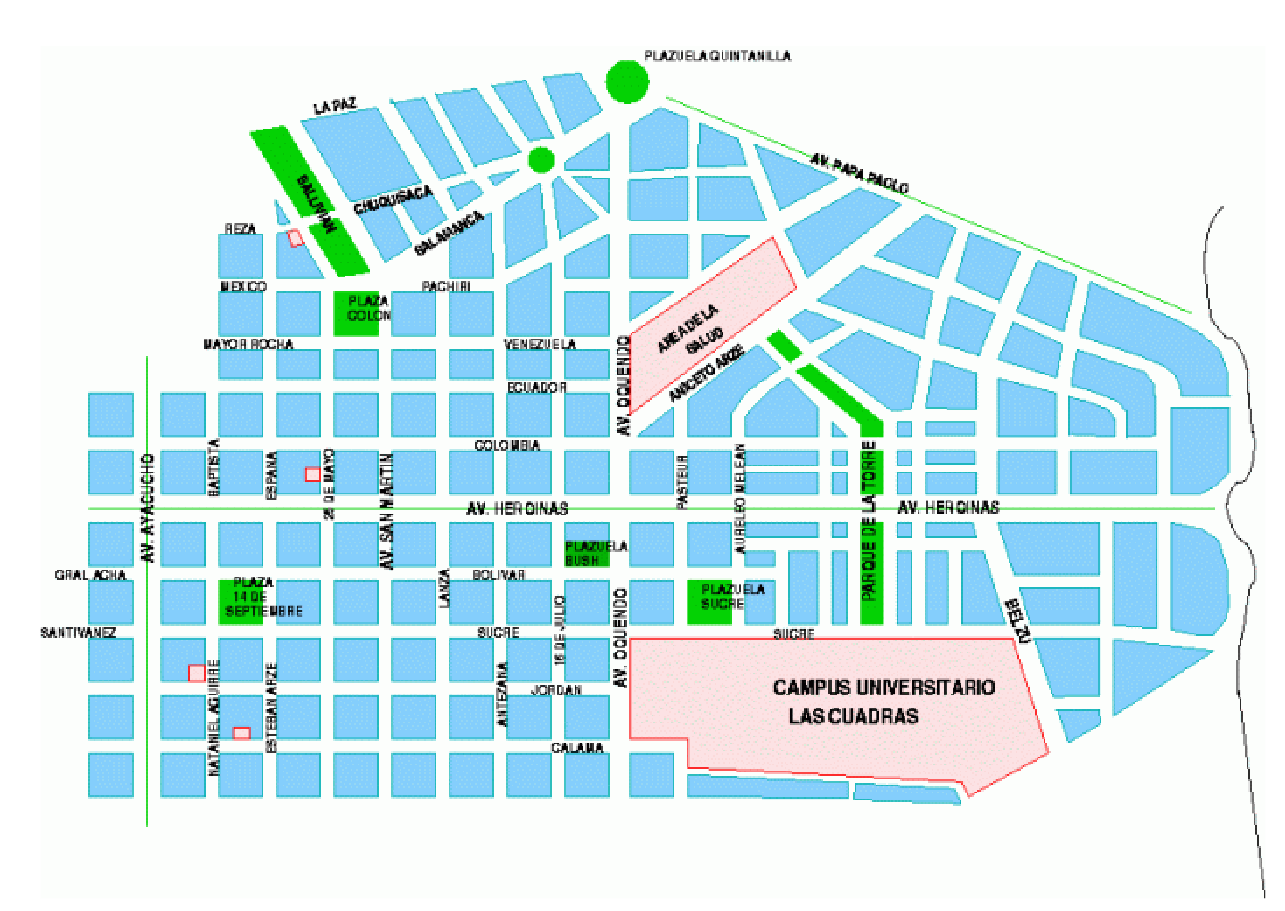
\includegraphics[width=0.75\textwidth]{mapa_old}
    \caption{Mapa universitario}
    \label{fig:mapa_old}
    \caption*{Fuente: \cite{umss_mapa}}
  \end{center}
\end{figure}


% Como personas que usamos los predios del campus ya sea como estudiantes, docentes o visitantes, todos necesitamos contar con un mapa más actualizado del campus universitario.\\
Los estudiantes, docentes y visitantes que usan y circulan dentro de los predios del campus, necesitan contar con un mapa más actualizado


Actualmente dentro del campus universitario ``Las Cuadras'' se puede encontrar las siguientes sectores:

\begin{enumerate}
\item FACH - Facultad de Arquitectura y Ciencias del Hábitat
% Dirección: Calle Jordán Interior
% Teléfonos: 4255730-4231172

\item FCJyP - Facultad de Ciencias Jurídicas y Políticas
% Dirección: Campus Central: Av. Oquendo esq Sucre
% Teléfonos: 591-4-4227509

\item FACES - Facultad de Ciencias Económicas
% Dirección: Edificio Prototipo I - Final Calama Este Campus Universitario
% Teléfonos: 4540245 - 4540248 - 4540261 FAX: 4540257


\item FHCE - Facultad de Humanidades y Ciencias de la Educación
% Dirección: Plaza Sucre acera Sud
% Teléfonos: 591-4-4544102

\item FCyT - Facultad de Ciencias y Tecnología
% Dirección: Calle Sucre y parque la Torre
% Teléfonos: 591-4-4231765

\item Multiacademico
\item Complejo Deportivo


\end{enumerate}

La Universidad cuenta con Aulas numeradas hasta el 758, repartidas entre todas las facultades y hasta para un estudiante que pasa gran parte de su tiempo dentro del campus es difícil encontrar un lugar cuando no se sabe su locación exacta, entonces para un visitante ocasional esto puede llegar a ser un gran problema.\\

Pero aparte de Aulas también se encuentra del campus, oficinas administrativas, centros de estudiantes, snacks, etc. por lo que conocer con exactitud la locación de un lugar es de gran importancia para no extraviarse dentro del campus universitario.\\


\begin{figure}[H]
  \begin{center}
    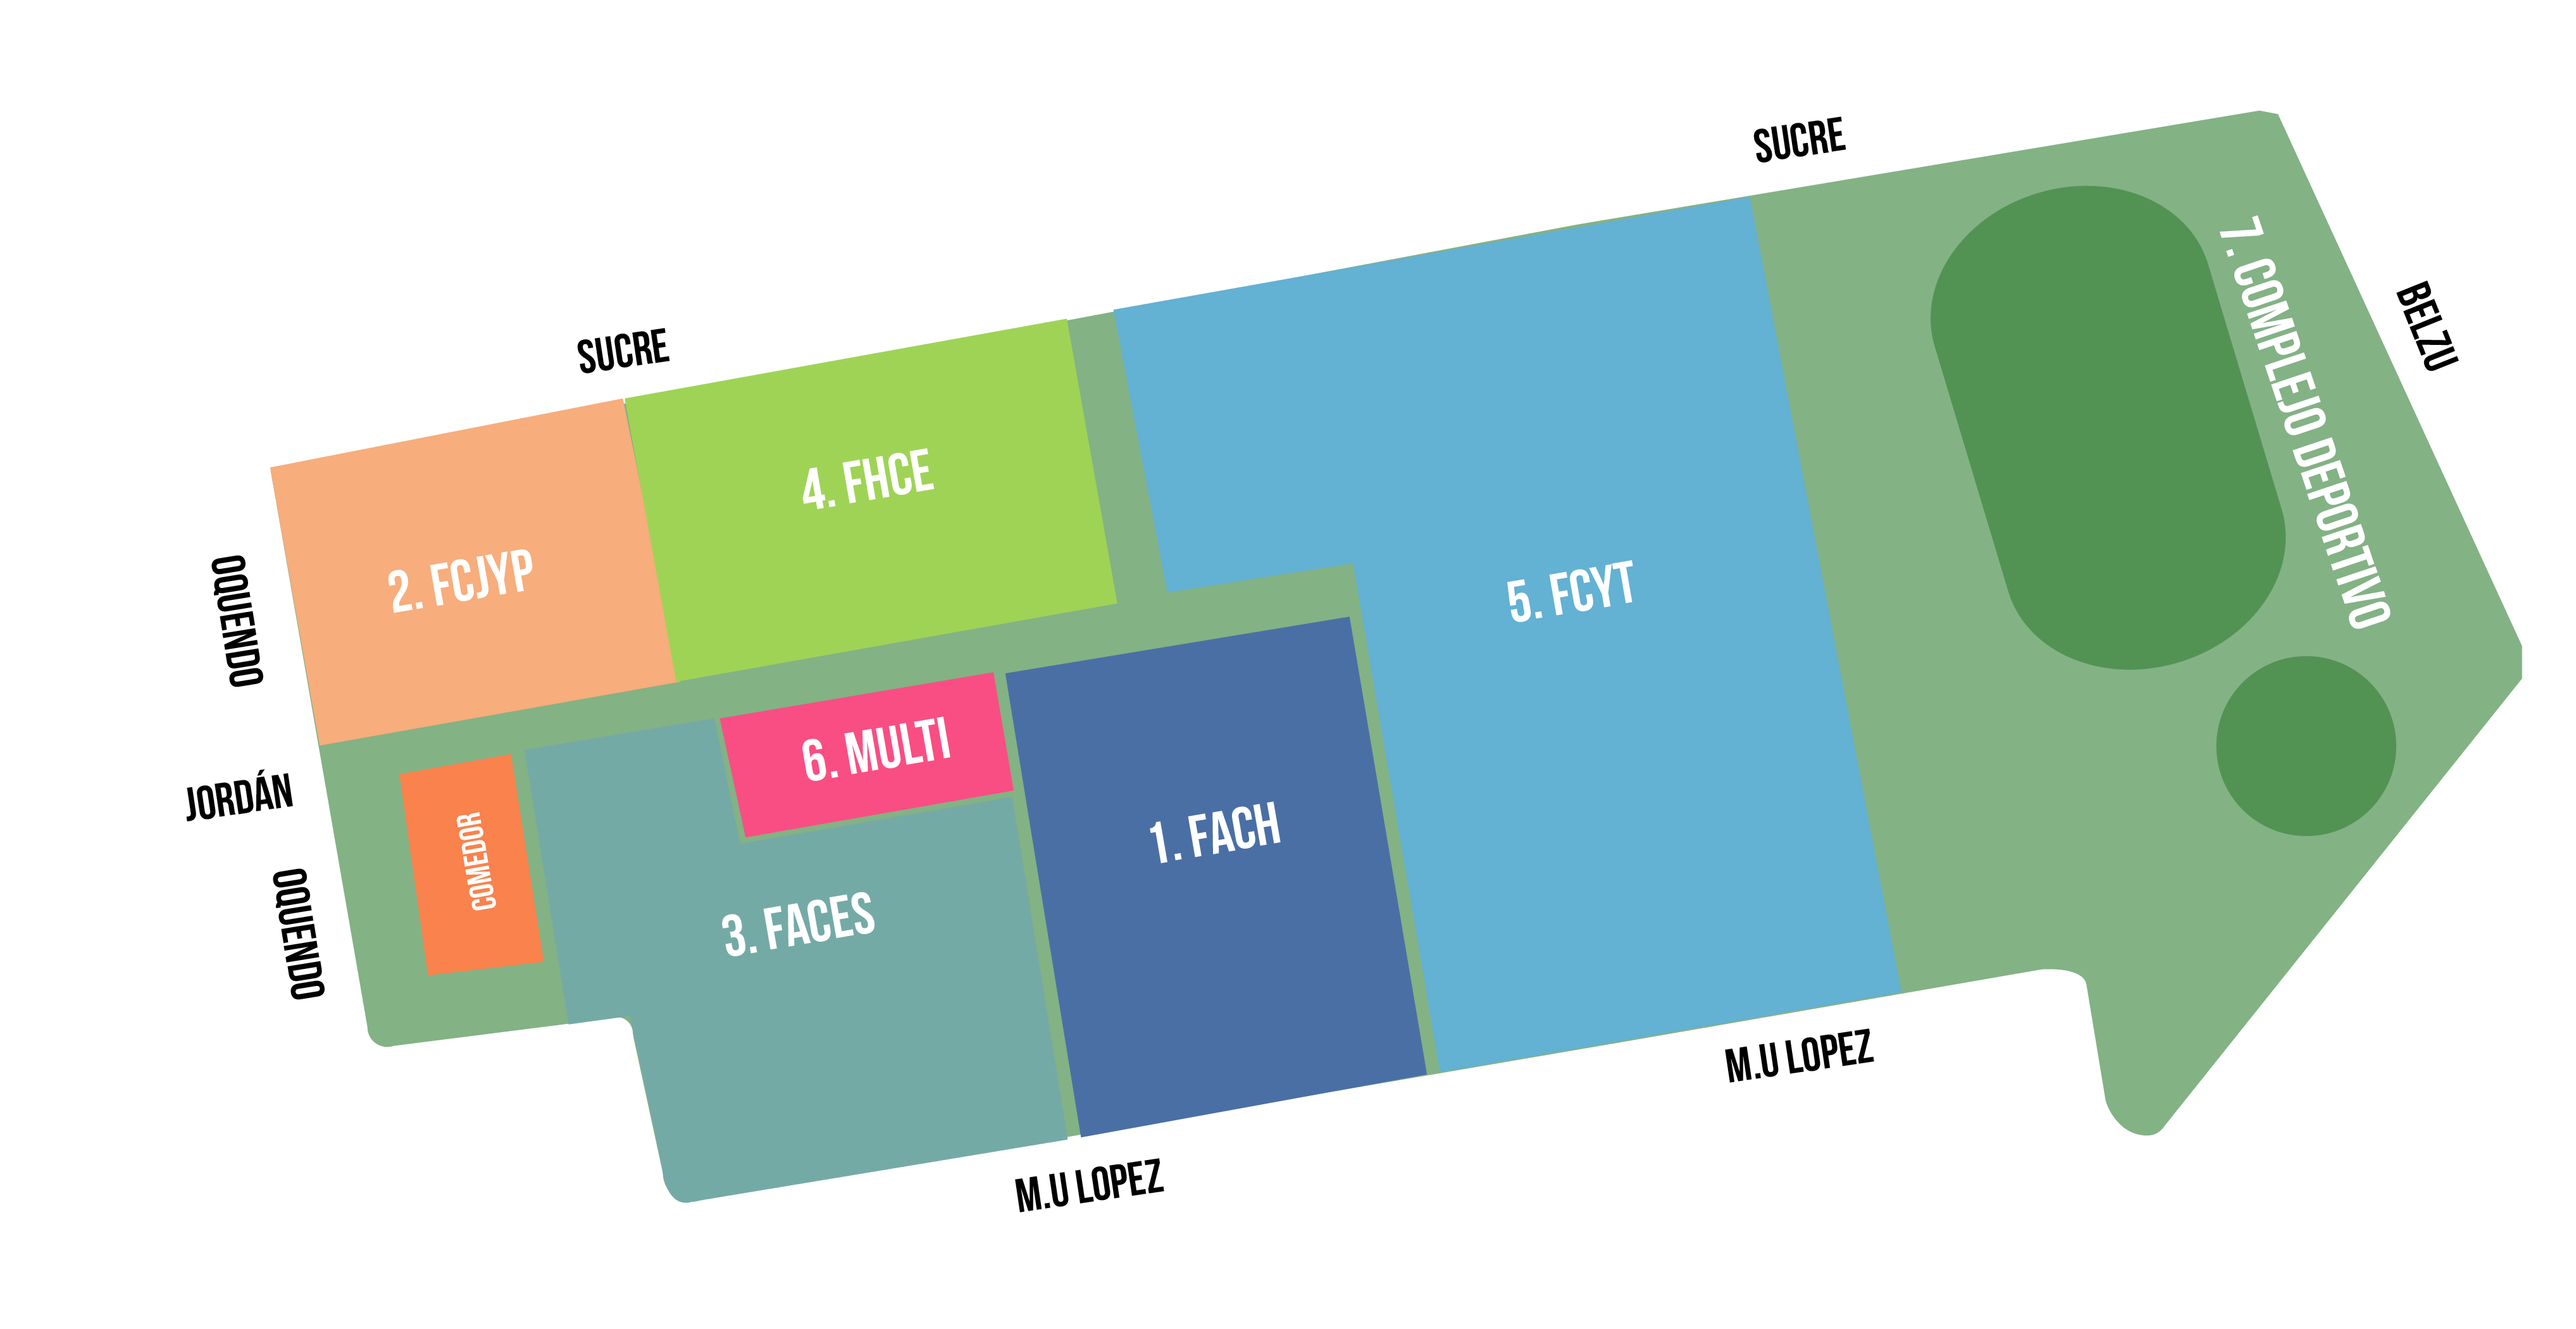
\includegraphics[width=1\textwidth]{mapa_new}
    \caption{Facultades dentro del Campus}
    \label{fig:mapa_new}
    \caption*{Fuente: Elaboración propia}

  \end{center}
\end{figure}


En la figura \ref{fig:mapa_new} se puede apreciar a grandes rasgos la distribución de las facultades dentro del campus, el mapa sirve para dar una idea de la ubicación de las facultades y edificios administrativos, los cuales son detallados a continuación.

\section{Facultad de Arquitectura y Ciencias del Hábitat}
\label{sec:facultad_arquitectura}

% Dirección: Calle Jordán Interior
% FACH - Facultad de Arquitectura y Ciencias del Hábitat
    La Facultad de Arquitectura y Ciencias del Hábitat colinda con la calle M. U. Lopez, dentro de los predios del campus Universitario se halla entre las facultades de Economía hacia el Sur-Este y con la facultad de Tecnología hacia el Nor-Oeste, en la figura \ref{fig:fac_arqui} se puede apreciar la facultad con las aulas y oficinas que cuenta en su interior.\\

    \begin{figure}[H]
     \begin{center}
       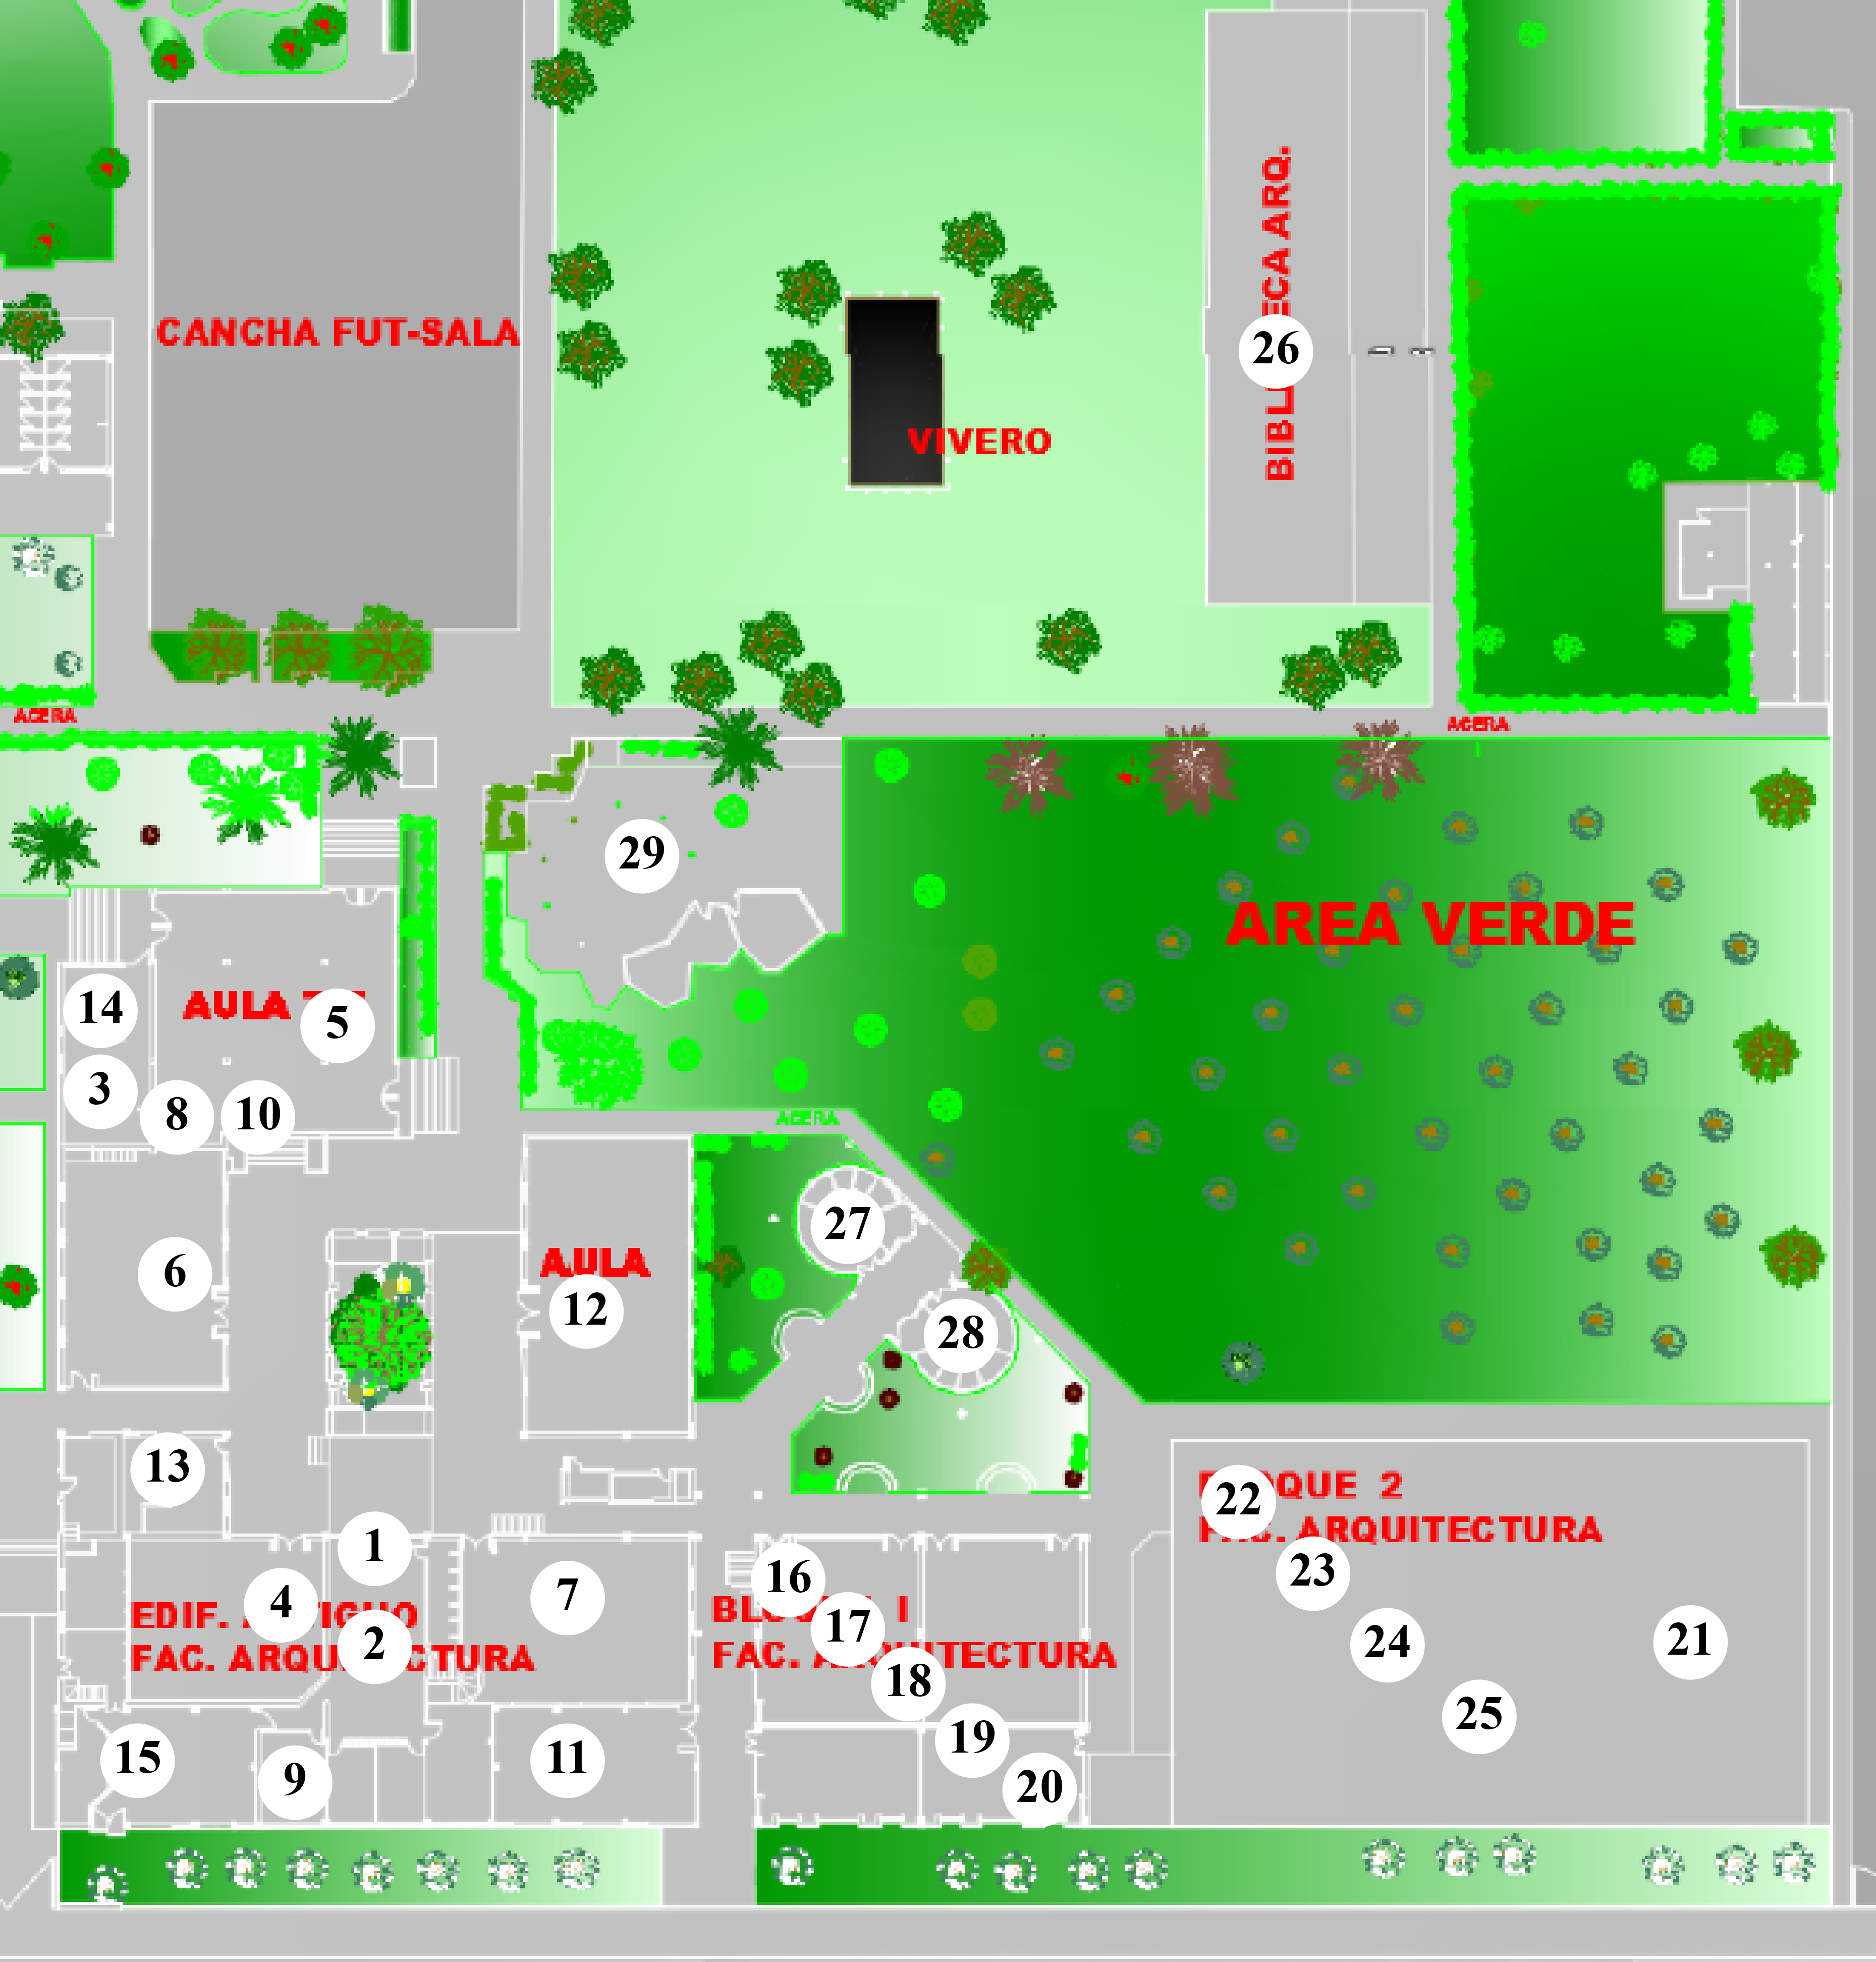
\includegraphics[width=0.8\textwidth]{fac_arquitectura}
       \caption{Facultad de Arquitectura - UMSS}
       \label{fig:fac_arqui}
       \caption*{Fuente: Departamento Infraestructura - UMSS}
     \end{center}
    \end{figure}

    % % \begin{table}
%   \begin{center}
    \begin{longtable}{ c  X }
      \toprule
        \textbf{Punto} &
        \textbf{Detalle}\\

      \midrule
      \endhead

  \textbf{1}
  &
  Decanato FACH
  \\

  \textbf{2}
  &
  Dirección Carrera Arquitectura
  \\

  \textbf{3}
  &
  Dirección Carrera Turismo
  \\

  \textbf{4}
  &
  Asociación Docente de Arquitectura
  \\

\textbf{5}
&
Aula 701
\\

\textbf{6}
&
Aula 702
\\

\textbf{7}
&
Aula 703
\\

\textbf{8}
&
Aula 704
\\

\textbf{9}
&
Aula 705
\\

\textbf{10}
&
Aula 706
\\

\textbf{11}
&
Aula 707
\\

% \textbf{12}
% &
% Aula 708*
% \\

\textbf{12}
&
Aula 709
\\


\textbf{13}
&
Centro de Estudiantes de Arquitectura
\\

\textbf{14}
&
Centro de Estudiantes de Turismo
\\


\textbf{15}
&
Laboratorio de Arquitectura
\\

\textbf{16}
&
Planta Baja - Aulas: 720, 721, 722, 723
\\

\textbf{17}
&
1{\tiny er} Piso - Aulas: 724, 725
\\

\textbf{18}
&
2{\tiny do} Piso - Aulas: 726, 727
\\


\textbf{19}
&
3{\tiny er} Piso - Aulas: 728. 729
\\



\textbf{20}
&
4{\tiny to} Piso - Direccion de Formacion Continua Grado y Postgrado FACH
\\



\textbf{21}
&
Planta Baja - Auditorio ``M.Sc. Arq. Brownie Mostajo Medinaceli''
\\



\textbf{22}
&
1{\tiny er} Piso - Aulas: 740, 741, 742, 743
\\




\textbf{23}
&
2{\tiny do} Piso - Aulas: 745, 746, 747, 748
\\




\textbf{24}
&
3{\tiny er} Piso - Aulas: 750, 751, 752, 753
\\

\textbf{25}
&
4{\tiny to} Piso - Aulas: 755, 756, 757, 758
\\


\textbf{26}
&
Biblioteca FACH
\\

\textbf{27}
&
Aula 729
\\

\textbf{28}
&
EDAV - Estudio de Artes Visuales
\\

\textbf{29}
&
Snack Arquitectura
\\

\textbf{A30}
&
2{\tiny do} Piso - Aulas: 760, 761, 762, 763 - Ver en el mapa del Multiacademico, figura \ref{fig:multiacademico}
\\

\textbf{A31}
&
Aulas: TODO* - Ver en el mapa de Tecnología, figura \ref{fig:fac_tecno}
\\


      \bottomrule
      \caption{Locaciones de la Fac. Arquitectura}
      \label{tab:lugares_arquitectura}
    \end{longtable}
%   \end{center}
% \end{table}

    \LTXtable{0.8\textwidth}{facultades/arquitectura}



 \section{Facultad de Ciencias Jurídicas y Políticas}
 \label{sec:facultad_derecho}

 % La facultad de Derecho cuenta con alrededor de 178 vértices y 88 aristas, está ubicada al nor-oeste del Campus Universitario, en la esquina de la calle Oquendo y Sucre, dentro del campus colinda con la facultad de Humanidades hacia el Nor-Este y hacia el Sur-Oeste está la facultad de Economía.

 Generalmente conocida como ``Facultad de Derecho'' se encuentra al nor-oeste del Campus Universitario, en la Av. Oquendo esquina Sucre. En la figura \ref{fig:fac_derecho} se puede ver las locación de los lugares que se puede encontrar dentro de esta facultad. \\

 \begin{figure}[H]
   \begin{center}
     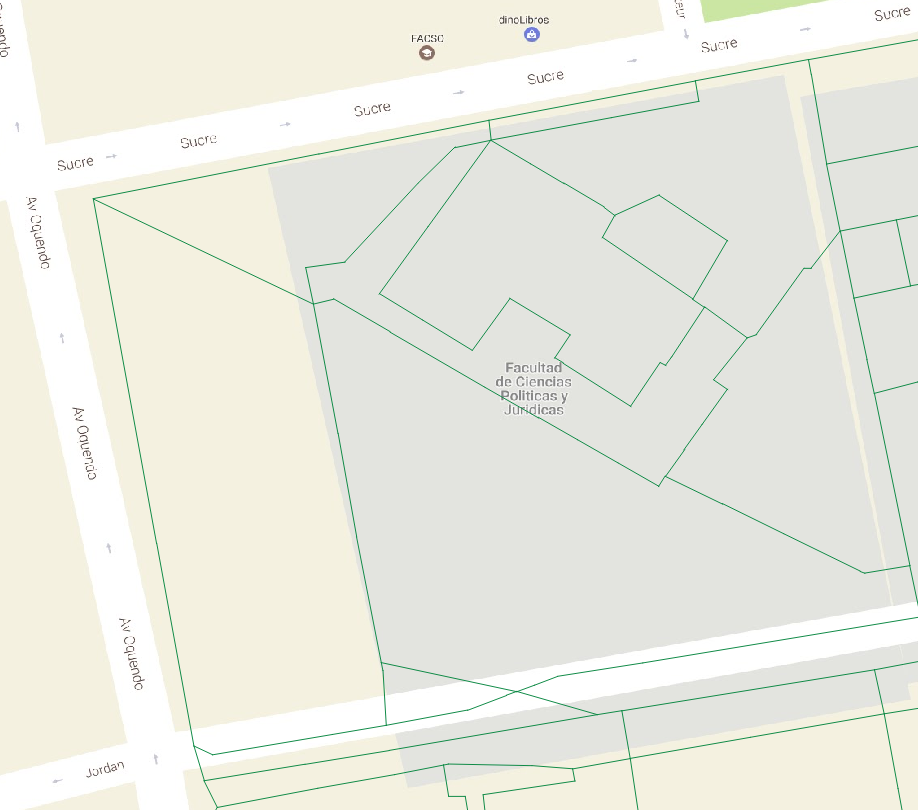
\includegraphics[width=0.8\textwidth]{fac_derecho}
     \caption{Facultad de Derecho - UMSS}
     \label{fig:fac_derecho}
     \caption*{Fuente: Departamento Infraestructura - UMSS}

   \end{center}
 \end{figure}

 \LTXtable{0.8\textwidth}{facultades/derecho}
 % \begin{table}[H]
  \begin{center}
    \begin{tabularx}{\textwidth}{ c  X }
      \toprule
        \textbf{Punto} &
        \textbf{Detalle}\\

      \midrule
        \textbf{1}
        &
        Centro de Estudiantes de Derecho
        \\

      \addlinespace
      \textbf{2}
      &
      1{\tiny er} Piso - Aula PP1, Aula PP2, Aula PP3, Aula PP4, Aula PP5, Aula PP6
      \\

      \addlinespace
      \textbf{3}
      &
      2{\tiny do} Piso - Aula SP1, Aula SP2, Aula SP3, Aula SP4, Aula SP5
      \\

      \addlinespace
      \textbf{4}
      &
      3{\tiny er} Piso - Carrera de Ciencia Politica
      \\

      \addlinespace
      \textbf{5}
      &
      3{\tiny er} Piso - Aula TP1, Aula TP2, Aula TP3, Aula TP4, Aula TP5
      \\

      \addlinespace
      \textbf{6}
      &
      3\text{\tiny er} Piso - Salon Auditorio ``Lic. Orlando Mercado Camacho''
      \\


      \addlinespace
      \textbf{7}
      &
      4{\tiny to} Piso - Aula CP1, Aula CP2, Aula CP3, Aula CP4, Aula CP5
      \\

      \addlinespace
      \textbf{8}
      &
      5{\tiny to} Piso - Aula QP1, Aula QP2, Aula QP3, Aula QP4, Aula QP5, Aula QP6
      \\

      \addlinespace
      \textbf{9}
      &
      Aula BA1
      \\

      \addlinespace
      \textbf{10}
      &
      Oficina Educativa Virtual Facultativa
      \\

      \addlinespace
      \textbf{11}
      &
      Full
      \\

      \addlinespace
      \textbf{12}
      &
      SITUMSS - Sindicato Trabajadores UMSS
      \\

      \addlinespace
      \textbf{13}
      &
      Snack Derecho
      \\

      \addlinespace
      \textbf{14}
      &
      Torre Fotos UMSS
      \\


      \bottomrule
    \end{tabularx}
    \caption{Locaciones de la Fac. Derecho}
    \label{tab:lugares_derecho}
  \end{center}
\end{table}




 % En la figura \ref{fig:fac_derecho} se puede observar en la línea verde los caminos o rutas dentro de la facultad de derecho de la UMSS, proyectada sobre el mapa de Google Maps, para lograr esta representación se utilizó QGIS ya que la información geográfica de la ruta está contenida en un archivo shapefile y el mapa se lo obtiene usando el API de Google Maps gracias al plugin de QGIS, \emph{QuickMapServices}.

 % \footnote{http://nextgis.com/blog/quickmapservices/}.




\section{Facultad de Ciencias Económicas}
\label{sec:facultad_economia}

      % Dirección: Edificio Prototipo I - Final Calama Este Campus Universitario
      La Facultad de Ciencias Económicas o comúnmente conocida como ``Facultad de Economía''
      colinda con las calles Oquendo y M. U. López, dentro del campus al Nor-Este se encuentra la facultad de Arquitectura y al Nor-Oeste la facultad de Derecho, tal como se puede apreciar en la figura \ref{fig:fac_economia}.

      \begin{figure}[H]
       \begin{center}
         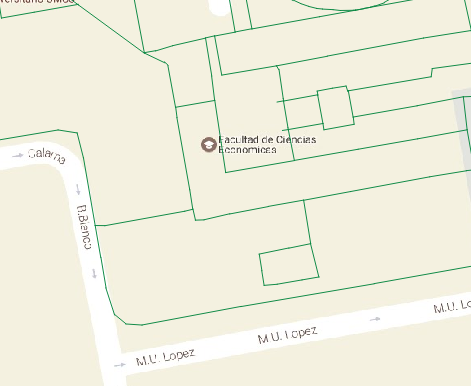
\includegraphics[width=1\textwidth]{fac_economia}
         \caption{Facultad de Economía - UMSS}
         \label{fig:fac_economia}
         \caption*{Fuente: Departamento Infraestructura - UMSS}

       \end{center}
      \end{figure}


      \LTXtable{0.8\textwidth}{facultades/economia}




\section{Facultad de Humanidades y Ciencias de la Educación}
\label{sec:facultad_humanidades}

La entrada a la facultad de Humanidades se lo encuentra sobre la calle Sucre en frente de la \emph{Plaza Sucre} acera Sud, en la figura \ref{fig:fac_humanidades} se puede apreciar la \emph{FHCE} dentro del campus Universitario y en la tabla \ref{tab:lugares_humanidades} se puede ver el detalle de los lugares que se pueden ubicar dentro de la facultad de Humanidades y Ciencias de la Educación.

\begin{figure}[H]
 \begin{center}
   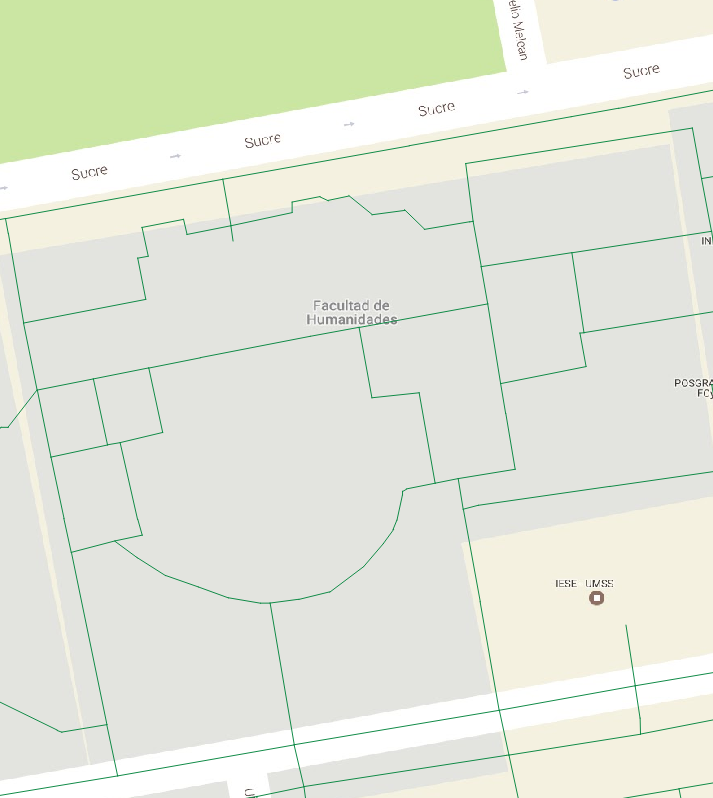
\includegraphics[width=0.75\textwidth]{fac_humanidades}
   \caption{Facultad de Humanidades - UMSS}
   \label{fig:fac_humanidades}
   \caption*{Fuente: Departamento Infraestructura - UMSS}
 \end{center}
\end{figure}

\LTXtable{0.8\textwidth}{facultades/humanidades}



\section{Facultad de Ciencias y Tecnología}
\label{sec:facultad_tecnologia}

Comúnmente conocida como ``facultad de Tecnología'',  se encuentra en el sector Nor-Este dentro del campus Universitario, se puede encontrar una entrada a la facultad de tecnología sobre la calle  al frente del parque \emph{la Torre} y otra entrada sobre la calle MU Lopez debajo de los edificios nuevos de tecnología, dentro del campus Universitario colinda con las facultades de Arquitectura y Humanidades que se encuentran hacia el Sur-Este y Sur-Oeste correspondientemente, en la siguiente figura \ref{fig:fac_tecno} se puede apreciar la facultad de Tecnología.

\begin{figure}[H]
 \begin{center}
   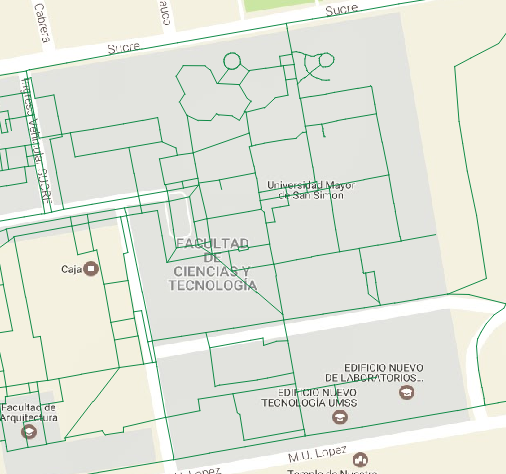
\includegraphics[width=0.9\textwidth]{fac_tecno}
   \caption{Facultad de Tecnología - UMSS}
   \label{fig:fac_tecno}
   \caption*{Fuente: Departamento Infraestructura - UMSS}
 \end{center}
\end{figure}

\LTXtable{0.8\textwidth}{facultades/tecnologia}
% % \begin{table}[H]
%   \begin{center}
    \begin{longtable}{ c  X }
      \toprule
        \textbf{Punto} &
        \textbf{Detalle}\\

      \midrule
      \endhead

    \textbf{1}
    &
    MEMI - Centro  de Mejoramiento de la enseñanza  de la Matemática y la Informática
    \\

      \textbf{2}
      &
        1{\tiny er} Piso - Postgrado FCyT - UMSS
      \\

      \textbf{3}
      &
      Auditorio MEMI
      \\

      \textbf{4}
      &
      Departamento Informática - Sistemas
      \\

      \textbf{5}
      &
      Laboratorio
      \\

      \textbf{6}
      &
      Parqueo Tecnologia
      \\

      \textbf{7}
      &
      Aula 623
      \\


      \textbf{8}
      &
      Aula 622
      \\

      \textbf{9}
      &
      Aula 624
      \\

      \textbf{10}
      &
      Biblioteca FCYT
      \\

      \textbf{11}
      &
      2{\tiny do} Piso - Proyecto CAE, Aula 625C, Aula 625D
      \\

      \textbf{12}
      &
      Auditorio Tecnologia
      \\

      \textbf{13}
      &
      Centro de Servicios
      \\

      \textbf{14}
      &
      Instituto de Investigaciones
      \\


      \textbf{15}
      &
      Cafe Docente - Tecnologia
      \\

      \textbf{16}
      &
      Departamento de Fisica, Aulas: 618, 619, 619A, 620, 620B, 621, 621A
      \\

      \textbf{17}
      &
      1{\tiny er} Piso - Aula 617
      \\

      \textbf{18}
      &
      Aula 617C, Aula 617B
      \\

      \textbf{19}
      &
      Departamento de Quimica, Aulas: 613, 614, 615, 616, 616A
      \\

      \textbf{20}
      &
      Aula 612
      \\

      \textbf{21}
      &
      Aula 607
      \\

      \textbf{22}
      &
      Departamento de Biologia, Aulas: 606, 608, 609, 608A, 608B, 609A
      \\

      \textbf{23}
      &
      Departamento de Industrial, Aulas: 631, 632
      \\

      \textbf{24}
      &
      Aula 635
      \\

      \textbf{25}
      &
      Aulas: 640, 642, 643
      \\

      \textbf{26}
      &
      1{\tiny er} Piso - Aulas 644, 644A
      \\

      \textbf{27}
      &
      3{\tiny er} Piso - Auditorio Civil
      \\

      \textbf{28}
      &
      Aulas: 651, 652
      \\

      \textbf{29}
      &
      1{\tiny er} Piso - Decanatura FCyT
      \\

      \textbf{30}
      &
      2{\tiny do} Piso - Auditorio Mecanica, Aula magna Civil
      \\

      \textbf{31}
      &
      Edificio ELEKTRO, Aulas: 667A, 667B, 668
      \\

      \textbf{32}
      &
      1{\tiny er} Piso - Aulas: 669A, 669B, 670
      \\

      \textbf{33}
      &
      2{\tiny do} Piso - Aulas: 671, 671A, 671B, 671C, 672
      \\

      \textbf{34}
      &
      3{\tiny er} Piso - Aulas: 674A, 674B, 675
      \\

      \textbf{35}
      &
      Planta Baja - Aulas: 690A, 690B, 690C, 690D
      \\

      \textbf{36}
      &
      1{\tiny er} Piso - Aulas: 691A, 691B, 691C, 691D, 691E, 691F
      \\

      \textbf{37}
      &
      2{\tiny do} Piso - Aulas: 692A, 692B, 692C, 692D, 692E, 692F, 692G, 692H
      \\

      \textbf{38}
      &
      3{\tiny er} Piso - Auditorio 2 FCyt, Aulas: 693A, 693B, 693C, 693D
      \\

      \textbf{39}
      &
      Planta Baja - Aulas: 680-A, 680-B, 680-C, 680-D, 680-E, 680-F, 680-G, 680-H, 680-I, 680-J, 680-K, 680-L, 680-M
      \\

      \textbf{40}
      &
      1{\tiny er} Piso - Aulas: 681-A, 681-B, 681-C, 681-D, 681-E, 681-F, 681-G, 681-H, 681-I, 681-J, 681-K, 681-L
      \\

      \textbf{41}
      &
      2{\tiny do} Piso - Aulas: 682-A, 682-B, 682-C, 682-D, 682-E, 682-F, 682-G, 682-H, 682-I, 682-J, 682-K, 682-L
      \\

      \textbf{42}
      &
      3{\tiny er} Piso - Aulas: 683-A, 683-B, 683-C, 683-D, 683-E, 683-F, 683-G, 683-H, 683-I, 683-J, 683-K, 683-L
      \\

      \textbf{43}
      &
      4{\tiny to} Piso - Biblioteca, Aulas: 684-A, 684-B, 684-C, 684-D, 684-E, 684-F, 684-G, 684-H, 684-I, 684-J, 684-K
      \\

      \textbf{44}
      &
      Centro de Aguas y Saneamiento Ambiental CASA
      \\

      \textbf{45}
      &
      Planta de Alimentos y Productos Naturales CAPN
      \\


      \textbf{46}
      &
      Planta de Tratamientos de Agua
      \\


      \textbf{47}
      &
      Departamento de Infraestructura
      \\


      \textbf{48}
      &
      Departamento de Mantenimento
      \\


      \textbf{49}
      &
      Centros CTA, CBG, Biotecnologia
      \\


      \textbf{50}
      &
      Planta Agroquimico
      \\


      \textbf{51}
      &
      Laboratorio de Materiales
      \\


      \textbf{52}
      &
      Planta Biogas (Biodigestor)
      \\

      \textbf{53}
      &
      Planta Amoniaco
      \\


      \textbf{54}
      &
      Laboratorio Simulacion Metodos y Seguridad
      \\

      \textbf{55}
      &
      Sub Estacion de Potencia
      \\

      \bottomrule
      \caption{Locaciones de la Fac. Tecnologia}
      \label{tab:lugares_tecnologia}
    \end{longtable}
%   \end{center}
% \end{table}


\section{Multiacademico}
\label{sec:multiacademico}

En la parte central del campus universitario se encuentra el edificio ``multiacademico'', el cual en su mayoría está compuesto por oficinas administrativas pero también se puede encontrar aulas, en la figura \ref{fig:multiacademico} se puede ver el mapa del edificio y en la tabla  \ref{tab:lugares_multiacademico} se describe el detalle de los ``lugares'' ubicados al interior del multiacademico.
\\

\begin{figure}[H]
 \begin{center}
   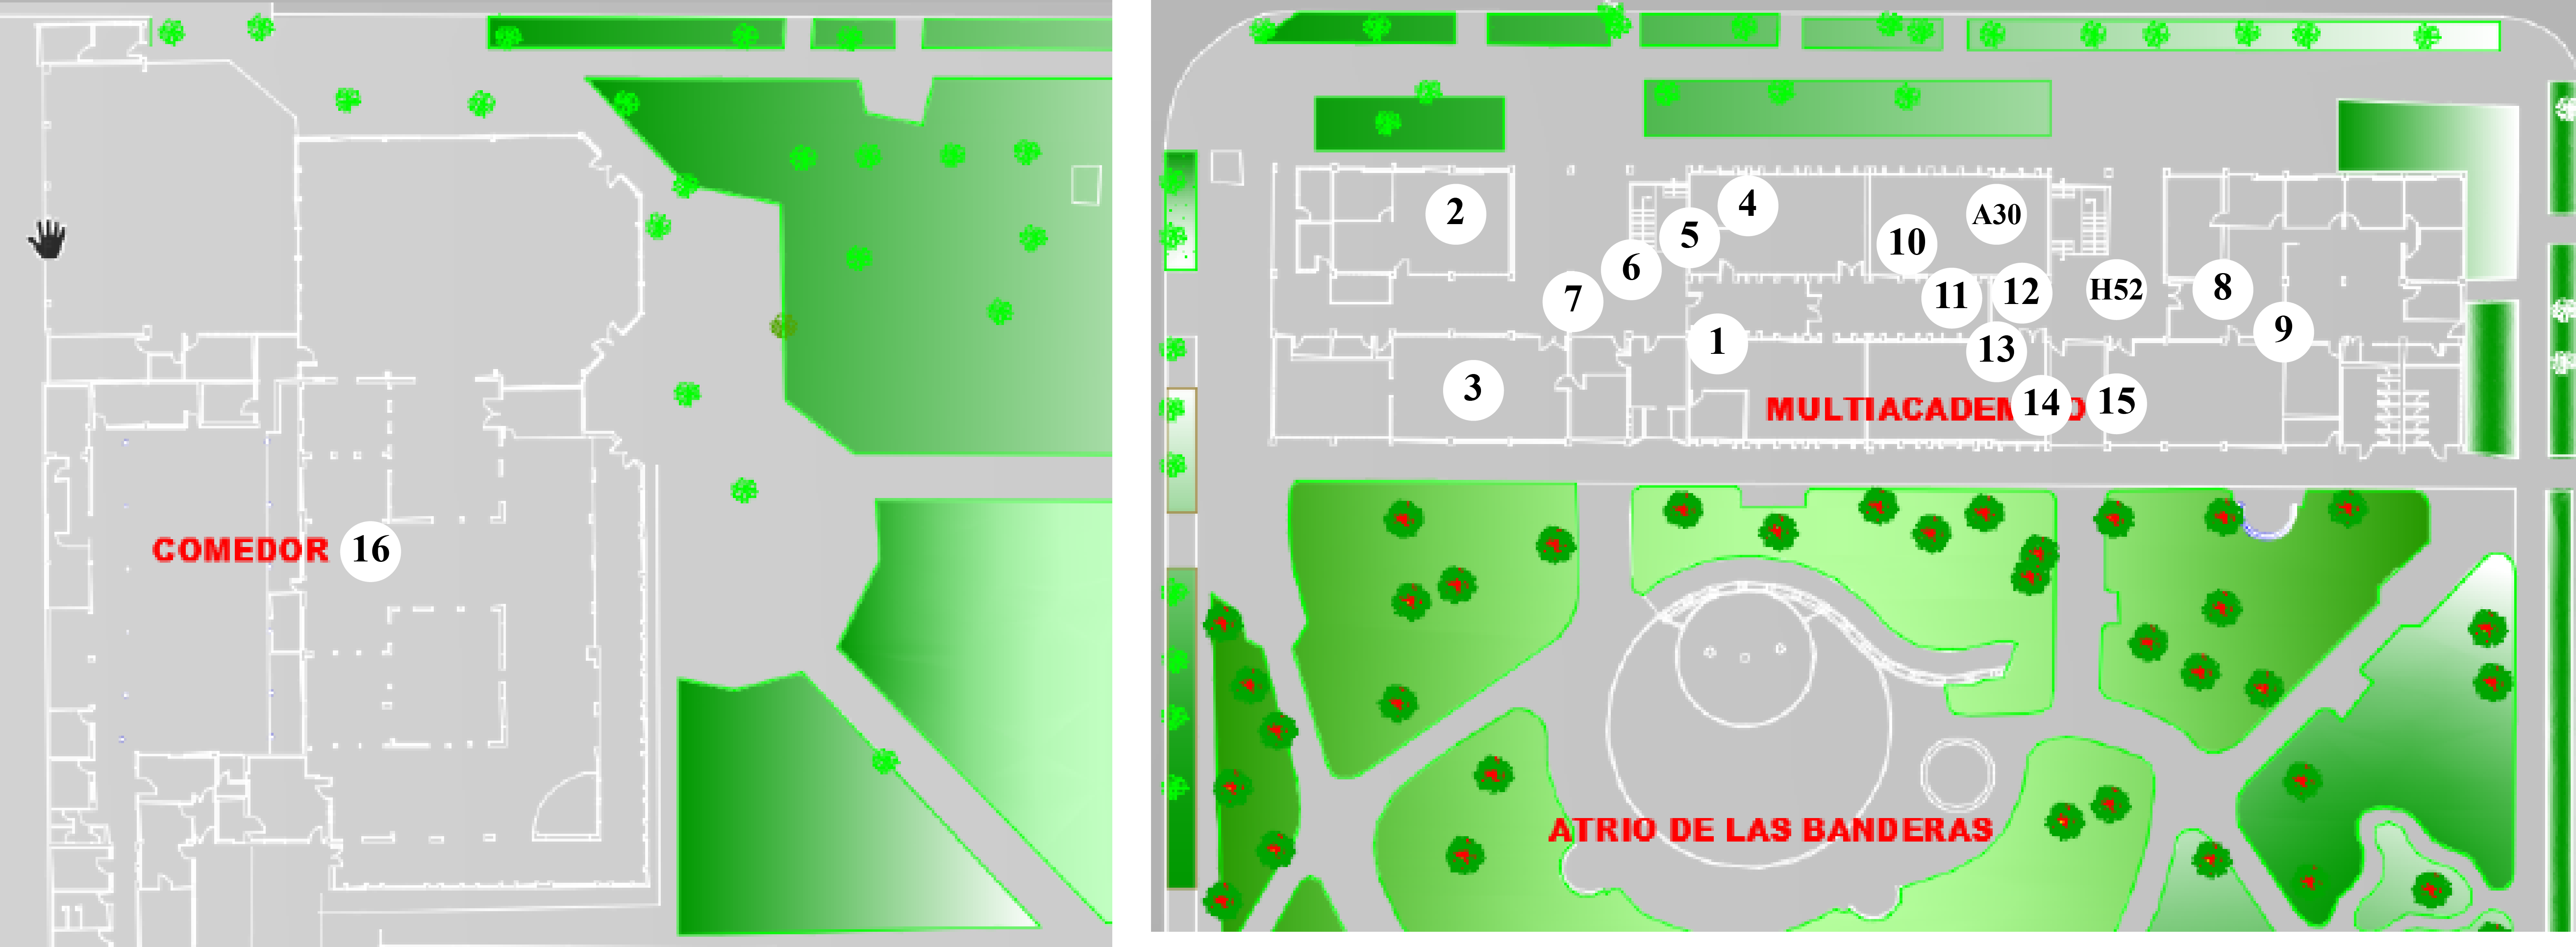
\includegraphics[width=0.9\textwidth]{multiacademico}
   \caption{Multiacademico - UMSS}
   \label{fig:multiacademico}
   \caption*{Fuente: Departamento Infraestructura - UMSS}
 \end{center}
\end{figure}

\newpage

\LTXtable{0.8\textwidth}{facultades/multiacademico}
% % \begin{table}
%   \begin{center}
    \begin{longtable}{ c  X }
      \toprule
        \textbf{Punto} &
        \textbf{Detalle}\\

      \midrule
      \endhead

\textbf{1}
&
PB - Unidad de Archivos Diplomas y Títulos (Legalizaciones)
\\

\textbf{2}
&
PB - Entrega de Diplomas
\\

\textbf{3}
&
PB - Departamento de Registros e Inscripciones
\\

\textbf{4}
&
1{\tiny er} Piso - DPA, Direccion de Planificacion Academica
\\


\textbf{5}
&
2{\tiny do} Piso - Planificación del Territorio y del Medio Ambiente
\\


\textbf{6}
&
3{\tiny er} Piso - Sala Consejo Universitario, Vice-Rectorado, PTAANG (Programa de Titulación de Alumnos Antiguos No Graduados)
\\


\textbf{7}
&
4{\tiny to} Piso - Jefatura de Personal Administrativo
\\


  \textbf{8}
  &
  PB - DISU (Dirección de Interacción Social Universitaria)
  \\

% \textbf{9}
% &
% PB - Aula 228 y Aula 229
% \\

\textbf{9}
&
1{\tiny er} Piso - Aula Internado Psicologia, Brigadas Universitarias de Salud
\\


\textbf{10}
&
1{\tiny er} Piso - PROTICS (Programa de Tecnologias de Informacion y Comunicacion Aplicadas a la Educación)
\\

% \textbf{6}
% &
% 1{\tiny er} Piso - Aulas: 233, 234, 237, 240, 241, 243
% \\

\textbf{11}
&
2{\tiny do} Piso - PROGEO (Programa de Geografía), Instituto de Investigaciones de Arquitectura, PROMESHA, Biblioteca IIACH
\\

\textbf{12}
&
2{\tiny do} Piso - CLAS (Centro de Levantamientos aeroespaciales y aplicaciones SIG para el desarrollo sostenible de los recursos naturales)
\\


\textbf{13}
&
3{\tiny er} Piso - DICyT (Dirección de Investigación Científica y Tecnológica)
\\



\textbf{14}
&
3{\tiny er} Piso - DUBE (Dirección Universitaria de Bienestar Estudiantil)
\\


\textbf{15}
&
4{\tiny to} Piso - DUEA (Dirección Universitaria de Evaluacion y Acreditacion - UMSS)
\\

\textbf{16}
&
Comedor Universitario
\\


\textbf{M17}
&
Caja Central UMSS (ver en el mapa de la Fac. Tecnologia, figura \ref{fig:fac_tecno})
\\


\textbf{M18}
&
Ofinica Almacenes Adquisiciones (ver en el mapa de la Fac. Tecnologia, figura \ref{fig:fac_tecno})
\\

      \bottomrule
      \caption{Locaciones del Multiacademico}
      \label{tab:lugares_multiacademico}
    \end{longtable}
%   \end{center}
% \end{table}


\newpage

\section{Complejo Deportivo}
\label{sec:canchas}

También podemos encontrar dentro del campus Universitario, el complejo deportivo cuyo mapa se puede ver en la figura \ref{fig:canchas} y el correspondiente detalle en la tabla \ref{tab:canchas}

\begin{figure}[H]
 \begin{center}
   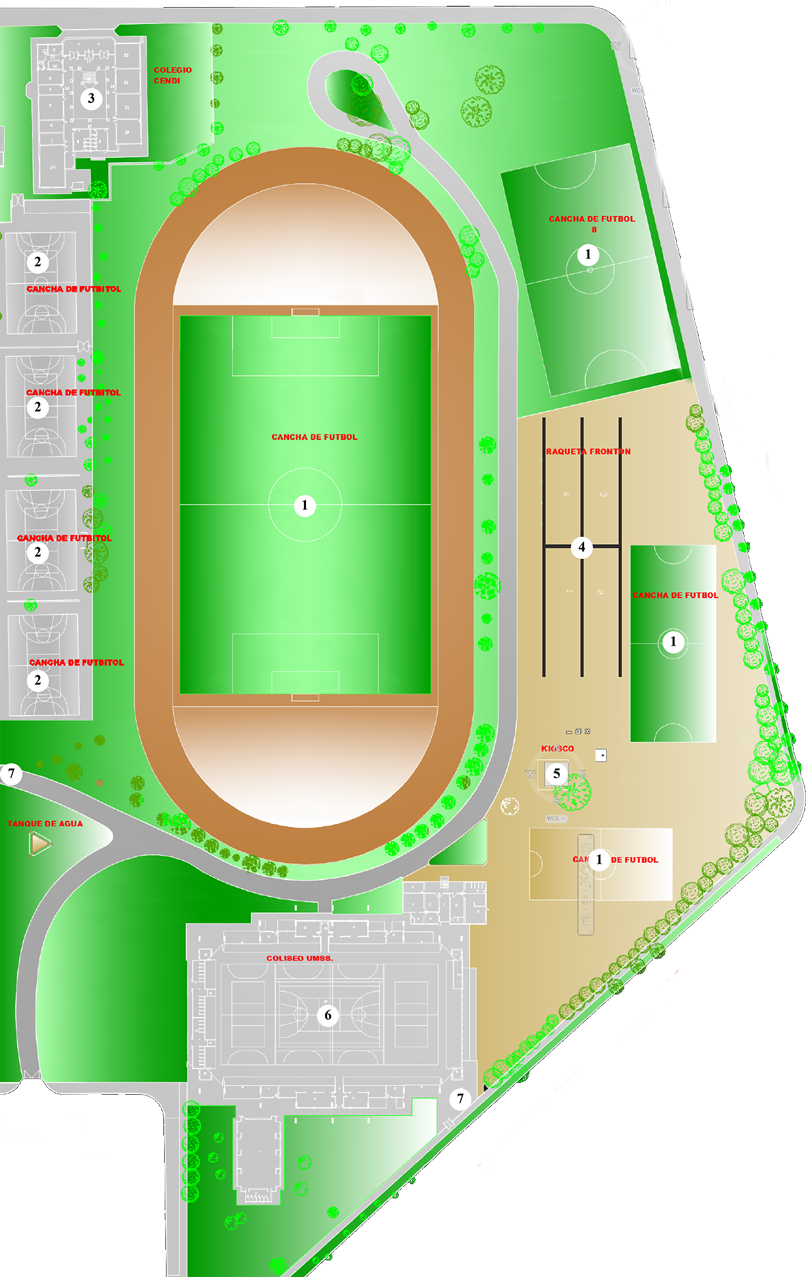
\includegraphics[width=0.5\textwidth]{canchas}
   \caption{Complejo Deportivo - UMSS}
   \label{fig:canchas}
   \caption*{Fuente: Departamento Infraestructura - UMSS}
 \end{center}
\end{figure}


\LTXtable{0.50\textwidth}{facultades/canchas}


\section{Facultades fuera del campus Universitario}
\label{sec:Facultades fuera del campus Universitario}

Las siguientes facultades no se hallan dentro del campus Universitario ``Las Cuadras'' por lo que escapan del alcance del presente proyecto de grado, pero se las nombrara para el conocimiento del lector.

\begin{description}
  \item[FACSO:] La Facultad de Ciencias Sociales o ``SOCIOLOGÍA'' está ubicada Nataniel Aguirre No. S 0360 entre Santivañez y Jordán, también conocida como ``Campus Sociología''.
  \item[FByF:] Facultad de Ciencias Farmacéuticas y Bioquímicas ubicada sobre Av. Aniceto Arce frente Parque La Torre.
  \item[FCAPFyV:] Facultad de Ciencias Agrícolas, Pecuarias, Forestales y Veterinarias
  Facultad de Ciencias Agrícolas, Pecuarias y Forestales ``Martin Cardenas'' (FCAPyP) ubicada en la Avenida Petrolera Km 5.
  \item[ODONTOLOGÍA:] Facultad de Odontología ubicada dentro el ``Campus Salud'', Calle Venezuela y Av. Oquendo.
  \item[MEDICINA:] Facultad de Medicina ubicada en el ``Campus Salud'', Av. Aurelio Melean 379.
  \item[FPVA:] Facultad Politecnica del Valle Alto ubicada en la Av. Mayor Rocha Provincia Punata.
  \item[FDRyT:] Facultad de Desarrollo Rural y Territorial  ubicada en la Av. Petrolera Km 5.5 carretera antigua a Santa Cruz.

\end{description}

% \item  - Facultad de Ciencias Sociales
% Dirección: Campus Sociología: Nataniel Aguirre No. S 0360 entre Santivañez y Jordán
% Teléfonos: 4502820 - 21 Fax: 4502821

% \item FByF - Facultad de Ciencias Farmacéuticas y Bioquímicas
% Dirección: Av. Aniceto Arce frente Parque La Torre
% Teléfonos: (591) (4) 420651 - (591) (4) 4250652


% FCAPFyV - Facultad de Ciencias Agrícolas, Pecuarias, Forestales y Veterinarias
%
% Dirección:
% Teléfonos: 4333808 - 4329666
%
% ODONTOLOGÍA - Facultad de Odontología
%
% Dirección: Campus Salud: C. Venezuela y Av. Oquendo
% Teléfonos: 4530307 - 4530314
% Fax. 4530314
%
% MEDICINA - Facultad de Medicina
%
% Dirección: Campus Salud: Av. Aurelio Melean 379
% Teléfonos: 4231508 - 4254910
%
% FPVA - Facultad Politecnica del Valle Alto
%
% Dirección: Av. Mayor Rocha Provincia Punata
% Teléfonos: (591)(4) 4577299
%
% FDRyT - Facultad de Desarrollo Rural y Territorial
%
% Dirección: Av. Petrolera Km 5.5 carretera antigua a Sta. Cruz
% Teléfonos: 4762387 - Telefax: 4761983


  
% \subsubsection{Implementar módulo para añadir lugares al sistema}
\subsubsection{Registro de Lugares en el sistema}

Para registrar un \emph{lugar} primeramente se implementó el formulario que se usará para recolectar la información del \emph{lugar}, el formulario fue creado usando \emph{EmberJs} y se lo puede ver en la figura \ref{fig:new_place}. \\

\begin{figure}[H]
     \begin{center}
       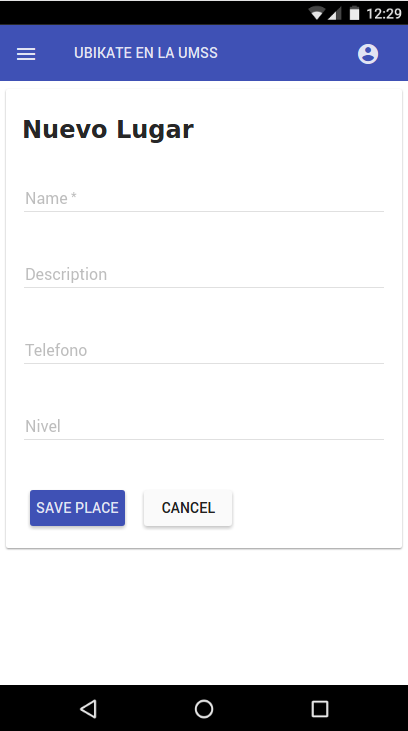
\includegraphics[width=0.3\textwidth]{new_place}

       \caption{Formulario para añadir un nuevo \emph{lugar}.}
       \label{fig:new_place}
       \caption*{Fuente: Elaboración propia.}
     \end{center}
\end{figure}

Posteriormente es necesario crear la petición HTTP desde el controlador de \emph{EmberJS} hacia el API, en el cuerpo de la petición se incluye la posición georeferenciada del celular utilizando el API de Geolocalización de HTML5 usada anteriormente para encontrar la ubicación del usuario, también se incluye el nombre, la descripción, el teléfono y el nivel del \emph{lugar}. En el codigo \ref{new_place_request} se puede ver la implementación de la petición.


% En la figura \ref{fig:new_place} se puede ver el formulario implementado usando \emph{ember-paper}, el cual colecciona los datos que se quieren introducir y se los envía al backend usando una llamada AJAX, como se puede ver en el siguiente código, para crear la petición POST se obtiene las coordenadas actuales del dispositivo móvil además de los datos recolectados del formulario y que con la ayuda de \emph{JQuery} es enviado al API el cual maneja la información recibida y se encarga de insertar los datos en la base de datos.\\

% \newpage
\begin{center}
 \begin{lstlisting}[label=new_place_request,caption=POST request creado en el controlador de \emph{ember}]

   var payload = {
       name: nombre,
       description: descripcion,
       phone: telefono,
       level: nivel,
       lat: latitud,
       lon: longitud
   };

   var url = (ENV.APP.API_HOST || '') + '/api/v1/places/';
   jQuery.post(url, payload).then(
       function(data) {
           var transition = controller.get('transition');
           if (transition) {
               self.transitionTo('places.show');
           } else {
               self.transitionTo('places');
           }
       },
       function(error) {
           controller.set('message', error.responseText);
       }
   );

 \end{lstlisting}
\end{center}

% En esta iteración se implementó la opción de añadir más lugares al sistema, de editarlos y eliminarlos, y la primera tarea es crear las consultas SQL para llevar a cabo las tareas. \\

% por lo que es necesario crear las consultas SQL que insertaran los datos enviados desde el dispositivo móvil al servidor. \\

% Como requisito para insertar un nuevo ``lugar'', se requiere que el usuario esté posicionado en el ``lugar'' ya que se usaran sus coordenadas para posicionar el ``lugar''. Las coordenadas del usuario son obtenidas usando el API de Geolocalización propia de HTML5, usada anteriormente para encontrar la ubicación del usuario \emph{visitante} en la iteración 2.\\

% Posteriormente se necesita implementar el formulario que el usuario usará para insertar los datos del ``lugar'': el nombre, la descripción, el teléfono y el nivel.\\

% Para insertar un ``lugar''  en la base de datos se usó el codigo \ref{new_place}, donde se puede observar la consulta SQL usada, para la cual se necesita capturar la latitud y longitud respectiva donde se encuentra el usuario, además de los datos del ``lugar''.\\

La petición creada es recibida en el API utilizando el \emph{endpoint} RESTful designado para ello, \verb|router.post('/', places.newPlace);|, el \emph{endpoint} se encarga de mandar la información recibida hacia la base de de datos, tomando en cuenta que la posición del lugar es un tipo especial de la base de datos, la latitud y longitud necesitan ser transformadas al momento de insertar el \emph{lugar} en la base de datos, como se muestra en el codigo \ref{cod-new_place_api}.


\begin{center}
 \begin{lstlisting}[label=cod-new_place_api,caption=Insertar un ``lugar'' en la base de datos.]

   router.post('/', places.newPlace);

   var newPlace = (req, res) => {
       var name = req.body.name || '';
       var lat = req.body.lat || '';
       var lon = req.body.lon || '';
       var description = req.body.description || '';
       var phone = req.body.phone || '';
       var level = req.body.level || '';

       let raw = `insert into place (name, geom, description, phone, level)
                  values ('${name}',
                          ST_GeomFromText('POINT(${lon} ${lat})', 3875),
                          '${description}',
                          '${phone}',
                          '${level}'
                         );`;

       Knex.raw(raw)
           .then(function(data) {
               res.json({
                   "message": "Place saved successfully!",
                   "data": data
               });
           })
           .catch(function(error) {
               res.send("Error:", error);
           });
   };

 \end{lstlisting}
\end{center}




% Para la creación de un ``lugar'' es necesario implementar un \emph{endpoint} en el API y siguiendo las convenciones REST se , para que como ya se explicó anteriormente el frontend pueda comunicarse con el backend. \\

% En el API de la aplicación, se implementó un \emph{endpoint} para que pueda manejar los \emph{request} del cliente para añadir un lugar, este \emph{request} es enviado usando el verbo HTTP \emph{POST}, que como ya se explicó es el usado en un REST API para crear objetos. \\

\subsubsection{Edición de la información del Lugar}

Para editar de la información de un lugar se rehusó el formulario ya creado para el registro del mismo, pero populando los campos con la información actual del lugar, el resultado se lo puede ver en la figura \ref{fig:place_edit_form}. \\

\begin{figure}[H]
     \begin{center}
       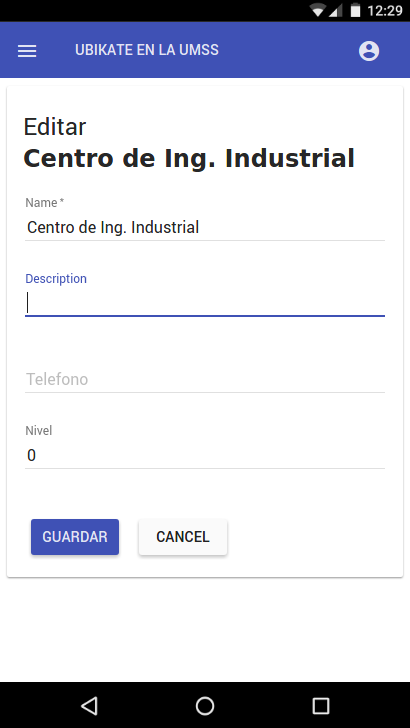
\includegraphics[width=0.3\textwidth]{place_edit_form}

       \caption{Formulario para editar un \emph{lugar}}
       \label{fig:place_edit_form}
       \caption*{Fuente: Elaboración propia.}
     \end{center}
\end{figure}


Los cambios a la información del \emph{lugar} son enviados al API mediante una petición PUT, siguiendo los lineamientos del REST API implementado, esta petición se puede ver en el codigo \ref{cod-edit_place_request}.

% \newpage
\begin{center}
 \begin{lstlisting}[label=cod-edit_place_request,caption=Petición HTTP para editar un lugar.]

   router.put('/:id', places.editPlace);

   var body = {
       name: name,
       description: description,
       phone: phone,
       level: level
   };

   var url = (ENV.APP.API_HOST || '') + `/api/v1/places/${id}`;
   jQuery.ajax({
       url: url,
       type: 'put',
       data: body
   }).then(
       function(data) {
           self.transitionTo('places.show', id);
       },
       function(error) {
           controller.set('message', error.responseText);
       }
   );

 \end{lstlisting}
\end{center}

A diferencia del registro del \emph{lugar}, que guarda la posición georeferenciada al momento de registrar el \emph{lugar}, en la edición de los datos no se está tomando en cuenta este dato porque se noto que generalmente cuando se requiere actualizar los datos del \emph{lugar}, el usuario no se encuentra en la posición original del \emph{lugar} y este dato se pierde, corrompiendo la base de datos. Es por esta razón que se decidió que no se actualizará la posición geográfica del \emph{lugar} sin alguna opción explícita que advierta al usuario de las consecuencias de esta acción, pero como tal tarea no se halla dentro de la \emph{historia de usuario} que se esta implementado, se tomo la decisión de realizarla en una futura iteración.








% \subsubsection{Eliminar un lugar}

% Una vez implementado la lógica para añadir un ``lugar'', se implementó los módulos para poder eliminar el ``lugar'', para esto se añadió un botón en la lista de lugares, el cual despliega un mensaje de advertencia al usuario de que está por eliminar un ``lugar'' y que la acción es irreversible, por lo tanto este botón sólo está disponible para un usuario \emph{administrador}. \\
%
% La verbo  HTTP \emph{DELETE} es el que de acuerdo a la implementación del API REST es el adecuado para eliminar un lugar, por lo tanto es el que se usó en la aplicación. En el codigo \ref{delete_place_enpoint} se puede observar el \emph{endpoint} implementado en el API que se encarga de manejar las peticiones \emph{DELETE} creando una consulta SQL que elimina el lugar de la base de datos.\\
%
% \begin{center}
%   \begin{lstlisting}[label=delete_place_enpoint,caption=DELETE request elimina un lugar.]
%
%     router.delete('/:id', places.deletePlace);
%
%     var deletePlace = (req, res) => {
%         var id = req.params.id;
%
%         Place.forge({
%             gid: id
%         })
%         .destroy()
%         .then(function(model) {
%             res.json({
%                 "message": "Place deleted successfully!"
%             });
%         })
%         .catch(function(err) {
%             res.status(500);
%         });
%     };
%
%   \end{lstlisting}
% \end{center}
%
% En el anterior codigo se puede apreciar la bondad de usar un manejador de bases de datos como \emph{Bookshelf} ya que usando el método \verb|destroy()|, se encarga automáticamente de crear la consulta SQL para eliminar una tupla de la base de datos.\\


  
\chapter{Conclusiones y Recomendaciones}

\section{Sobre la geolocalizacion}


    Es importante entender las diferencias entre los distintos tipos de sistemas de coordenadas porque computacionalmente realizar operaciones sobre los sistemas de coordenadas tiene costo. \\

          Si se usara el sistema de coordenadas geográfico (WSG84) este es el más apropiado si se necesitaría usar grandes extensiones de la superficie terrestre, que al ser una estructura elipsoidal el costo computacional para realizar las operaciones matemáticas de calcular distancias, intersecciones, etc. es más elevado. En cambio el uso de un sistema de coordenadas proyectado (Mercator Projection) tiene un costo computacional más bajo, ya que se estaría trabajando con un sistema geométrico.\\

          % Por otro lado,
          También hay tomar en cuenta la base de datos, ya que será esta la que se encargará de manejar los datos espaciales. Al estar usando PostGIS, se puede ver que en su documentacion\footnote{ http://postgis.org/documentation/manual-1.5/ch04.html} que claramente exorta el uso de un sistema geometrico sobre el uso de un sistema geografico si  se va trabajar con datos que cubran una pequena area geografica. Tomando en cuenta esta recomendación y el tamaño del área de estudio (el campus de la UMSS), se procedió a implementar en la base de datos el uso de la proyección Mercator. Se va usar Mercator sobre las otras proyecciones porque aparte de las ventajas que se mencionaron con anterioridad, Google Maps usa esta proyección y ya que se usará este mapa lo más correcto es trabajar con la misma proyección.


  \bibliographystyle{apacite}
  \bibliography{bibliografia}


  \begin{appendices}

  \appendix
  \addappheadtotoc
  \appendixpage

  \makeatletter
    \addtocontents{toc}{\let\protect\l@chapter\protect\l@section}
    \def\toclevel@chapter{1}
    \def\toclevel@section{2}
    \def\toclevel@subsection{3}
  \makeatother
    
\chapter{Manual Instalación}

El Manual de instalación tomará en cuenta que todos los comandos y las herramientas son ejecutados sobre un servidor Linux Ubuntu 16.04 LTS.

\section{Instalación de la base de datos}


\begin{itemize}
  \item \textbf{PostgreSQL:} Se usará la versión 9.4.8.

  \begin{center}
    \begin{lstlisting}[label=postgres_install,caption=Comandos usados para instalar PostgreSQL.]

      $ sudo apt-get update
      $ sudo apt-get install -y postgresql postgresql-contrib
    \end{lstlisting}
  \end{center}

  \item \textbf{PostGIS:} Se usará la versión 2.1.

  \begin{center}
    \begin{lstlisting}[label=postgis_install,caption=Comandos usados para instalar PostGIS.]

      $ sudo add-apt-repository ppa:ubuntugis/ubuntugis-unstable
      $ sudo apt-get install -y postgis postgresql-9.4-postgis-2.1
    \end{lstlisting}
  \end{center}

  \item \textbf{PgRouting:} Se usará la versión 2.2.

  \begin{center}
    \begin{lstlisting}[label=pgRouting_install,caption=Comandos usados para instalar PgRouting.]

      $ sudo add-apt-repository ppa:georepublic/pgrouting-unstable
      $ sudo apt-get update
      $ sudo apt-get install postgresql-9.4-pgrouting
    \end{lstlisting}
  \end{center}




\end{itemize}

\section{Configuración de la base de datos}


\begin{itemize}
  \item Habilitar \emph{Admin pack} en PostgreSQL.
  \begin{center}
    \begin{lstlisting}[label=adminpack,caption=Habilitar Admin Pack.]

      $ sudo -u postgres psql
      > CREATE EXTENSION adminpack;
      > \q
    \end{lstlisting}
  \end{center}

  \item Crear el Usuario de la Base de Datos y crear la Base de Datos usando el usuario creado.
  \begin{center}
    \begin{lstlisting}[label=adminpack,caption=Comandos para crear el usuario y la base de datos.]

      $ sudo -u postgres createuser -d -E -i -l -P -r -s USER_NAME
      $ sudo -u postgres createdb -O USER_NAME DATABASE_NAME
    \end{lstlisting}
  \end{center}


\end{itemize}


\subsection{Añadir las funciones de PostGIS y pgRouting a la base de datos}


PostGIS y pgRouting son extensiones a la base de datos PostgreSQL, y al instalar sus paquetes, todas las funciones que vienen con las extensiones están disponibles pero para utilizarlas hay que habilitarlas específicamente en la base de datos que las va a utilizar.


% Para habilitar la base de datos es necesario correr el siguiente comando en la terminal.
Ejecutar el siguiente comando para habilitar las funciones de PostGIS y pgRouting en la base de datos.

\begin{center}
  \begin{lstlisting}[label=enable_extensions,caption=Habilitación de las Extensiones.]

        $ sudo -u postgres psql -c ``
            CREATE EXTENSION adminpack; CREATE EXTENSION postgis;
            CREATE EXTENSION postgis_topology;
            CREATE EXTENSION pgrouting;
            CREATE EXTENSION fuzzystrmatch;
            CREATE EXTENSION postgis_tiger_geocoder;
         `` DATABASE_NAME
  \end{lstlisting}
\end{center}


\begin{itemize}
  \item Se puede verificar que las extensiones instaladas están correctamente habilitadas en la base de datos.
  \begin{center}
    \begin{lstlisting}[label=enable_extensions,caption=Habilitación de las Extensiones.]

          $ psql -h localhost -U USER_NAME DATABASE_NAME

          > SELECT postgis_full_version();
          > SELECT * FROM pgr_version();
    \end{lstlisting}
  \end{center}

\end{itemize}


\subsection{Habilitar el acceso a la base de datos}

PostgreSQL por defecto viene con la configuración habilitada para conectarse a la base de datos usando conexiones seguras. Pero  para el presente proyecto se debe ampliar los permisos de acceso a la base de datos para que el servicio REST API desarrollado no presenta problemas en la conexión a la base de datos.

\begin{itemize}
  \item Editar el archivo \emph{pg\_hba.conf} ubicado en el directorio de instalación de PostgreSQL. La última sección del archivo debe quedar como en la siguiente tabla.

  \begin{center}
    \begin{tabularx}{0.75\textwidth}{ X X X X X}
      \toprule
      hostssl &  all      &       all       &     0.0.0.0/0       &        md5 \\
      local &  all       &      postgres    &                     &       trust \\
      local &  all       &     all         &                      &      trust \\
      host  &  all        &     all        &     127.0.0.1/32      &      trust \\
      host  &  all       &      all        &     ::1/128           &      trust \\
      \bottomrule
    \end{tabularx}
    % \caption{Tarea de Ingeniería - T037}
    % \label{tab:T037}
  \end{center}

\item Reiniciar el servicio de PostgreSQL para que los cambios a la configuración tomen efecto.
\begin{center}
  \begin{lstlisting}[label=postgresql_restart,caption=Comando para reiniciar el servicio PostgreSQL.]

        $ sudo service postgresql restart
  \end{lstlisting}
\end{center}


\end{itemize}



\section{Configuration de la aplicación UBIKATE UMSS}

Para el presente proyecto se utilizaron los siguientes datos para configurar la base de datos.

\begin{itemize}
  \item USER\_NAME: db\_admin
  \item DATABASE\_NAME: db\_ubikate
\end{itemize}


\subsection{Instalación de las dependencias}

% A continuación se detallara los paquetes necesarios para correcta ejecución de la aplicación.
Instalar los siguientes paquetes para la correcta ejecución de la aplicación.

\begin{itemize}
  \item \textbf{NodeJS:} Se usará la versión 6.2.2 o superior.
  \begin{center}
    \begin{lstlisting}[label=node_install,caption=Comando para instalar NodeJS.]

          $ sudo apt-get install nodejs
    \end{lstlisting}
  \end{center}


  \item \textbf{Knex:} Instalar la última versión.
  \begin{center}
    \begin{lstlisting}[label=knex_install,caption=Commando para instalar Knex.]

          $ npm install knex -g
    \end{lstlisting}
  \end{center}

\end{itemize}


\subsection{Copiar los archivos del proyecto UBIKATE UMSS}

Los archivos de proyecto irán dentro de una carpeta, localizarla en alguna ubicación donde el usuario tenga permisos de lectura y escritura.

\subsection{Configurar el mapa topológico del campus Universitario}

El \emph{shapefile} con las rutas están ubicadas dentro de la carpeta \emph{resources} ubicada en la raíz del proyecto.

Para configurar la base de datos con los rutas se debe seguir los siguientes pasos:
\begin{enumerate}
  \item Popular la tabla correspondiente a las rutas.

\begin{center}

  \begin{lstlisting}[label=psql_ways,caption=Comando popular la base de datos.]

        $ psql -d db_ubikate -U db_admin -f resources/ways.sql
  \end{lstlisting}
\end{center}

      \item Añadir las columnas \emph{source} y \emph{target} a la tabla \emph{ways}, necesarias para agregar la topología.


\begin{center}

  \begin{lstlisting}[label=add_columns,caption=Agregar las columnas \emph{source} y \emph{target}.]

        $ psql -h localhost -U db_admin db_ubikate
        > alter table ways add column "source" integer;
        > alter table ways add column "target" integer;
  \end{lstlisting}
\end{center}

  \item Crear la topología usando pgRouting.

\begin{center}
  \begin{lstlisting}[label=add_topology,caption=Añadir la topología.]

        > select pgr_createTopology('ways', 0.00000001, 'geom', 'gid');
  \end{lstlisting}
\end{center}

\end{enumerate}

\subsection{Instalar las dependencias del proyecto UBIKATE UMSS}

Una vez los archivos hayan sido copiados, es necesario instalar todas las dependencias utilizadas por el proyecto.


\begin{center}
  \begin{lstlisting}[label=npm_install,caption=Instalar dependencias de la aplicación.]

        $ npm install
  \end{lstlisting}
\end{center}

\subsection{Iniciar el servidor \emph{ExpressJS}}

Finalmente se inicia el servidor \emph{ExpressJS} y la aplicación es mandada al cliente visitando la dirección del servidor.

\begin{center}
  \begin{lstlisting}[label=npm_start,caption=Iniciar el servidor.]

        $ npm start
  \end{lstlisting}
\end{center}

    \chapter{Manual Usuario}

\section{Página de Inicio}

Es la primera vista, ver figura \ref{fig:home_view}, que se despliega cuando accedemos a la aplicación, se puede ver una descripción del sistema implementado, se pueden apreciar los siguientes elementos:

\begin{enumerate}
  \item Icono del Menú.
  \item Icono del Login o Registro del Usuario.
  \item Botones de Registro de Usuario y Login respectivamente.
\end{enumerate}

\begin{figure}[H]
      \begin{center}
        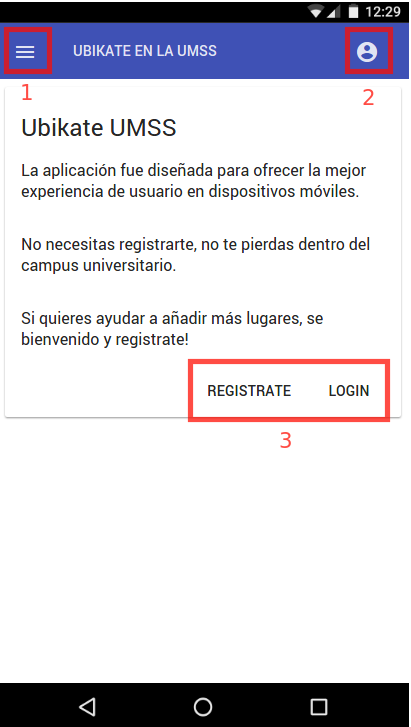
\includegraphics[width=0.3\textwidth]{manual_usuario/home}

        \caption{Página de Inicio.}
        \label{fig:home_view}
        \caption*{Fuente: Elaboración propia.}
      \end{center}
\end{figure}

\section{Menu de la Aplicación}

Está ubicado en el sección izquierda de la pantalla, se accede a ella haciendo un tap sobre el \emph{icono del Menú}, ver la figura \ref{fig:menu_view}. Una vez que se selecciona cualquier opción del menú, este se oculta. De esta forma se aprovecha el espacio reducido que dispone un dispositivo móvil.


\begin{figure}[H]
      \begin{center}
        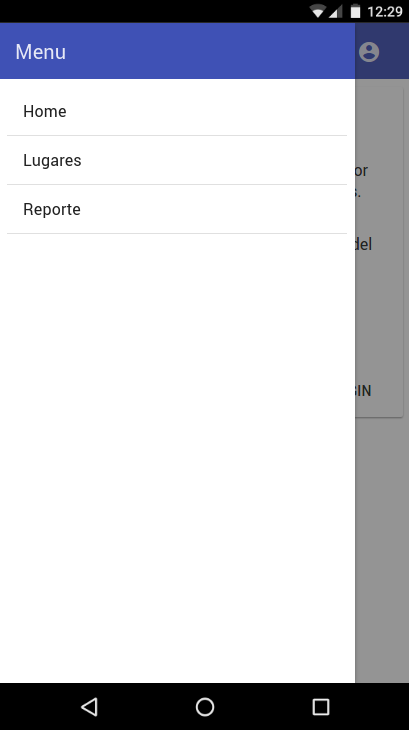
\includegraphics[width=0.3\textwidth]{manual_usuario/menu}

        \caption{Menú de la aplicación.}
        \label{fig:menu_view}
        \caption*{Fuente: Elaboración propia.}
      \end{center}
\end{figure}


\section{Lista de Lugares}

Se accede a la \emph{lista de lugares}, ver figura \ref{fig:vista_lugares}, seleccionando la opción \emph{Lugares} del Menú.

En la \emph{lista de lugares} se puede ver los siguiente elementos:

\begin{enumerate}
  \item Cajón de Búsqueda.
  \item Lista de Lugares.
  \item Botón de Registro de un Lugar (ver figura \ref{fig:vista_search}).
\end{enumerate}

\begin{figure}[H]
      \begin{center}
        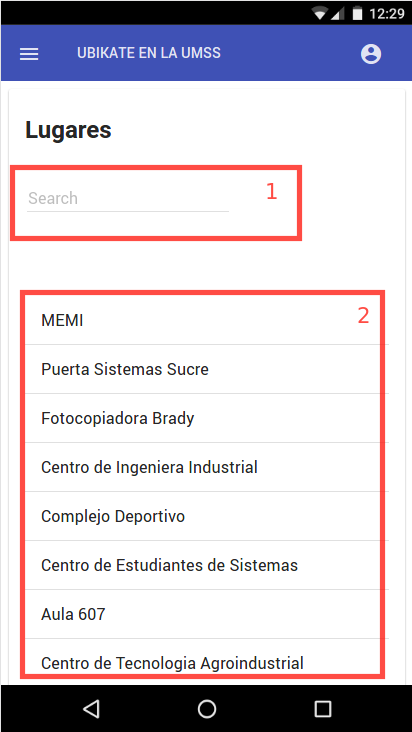
\includegraphics[width=0.3\textwidth]{manual_usuario/lugares}

        \caption{Lista de lugares.}
        \label{fig:vista_lugares}
        \caption*{Fuente: Elaboración propia.}
      \end{center}
\end{figure}

\begin{itemize}
  \item \textbf{Cajón de Búsqueda:} La lista de lugares es filtrada de acuerdo al nombre de un lugar o parte del nombre, que es ingresada en el \emph{cajón de búsqueda}. Como se puede apreciar en la figura \ref{fig:vista_search}.

  \begin{figure}[H]
        \begin{center}
          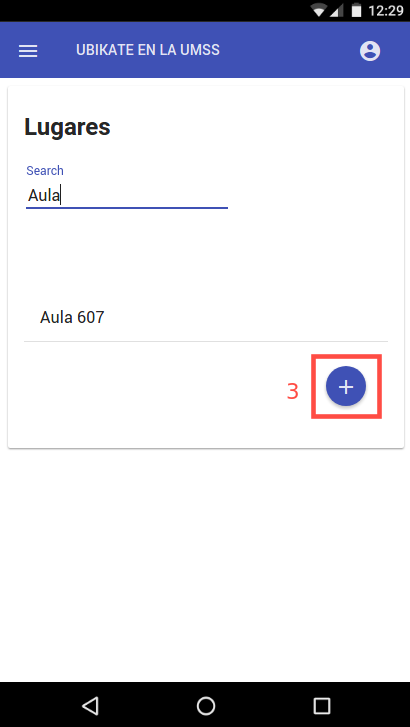
\includegraphics[width=0.25\textwidth]{manual_usuario/search}

          \caption{Cajón de Búsqueda.}
          \label{fig:vista_search}
          \caption*{Fuente: Elaboración propia.}
        \end{center}
  \end{figure}

  \item \textbf{Lista de Lugares:} Es la lista de lugares propiamente dicha, contiene todos los lugares registrados en la aplicación o la lista filtrada mediante el \emph{cajón de búsqueda}.

\item \textbf{Botón de Registro de un Lugar:} Ubicada al final de la \emph{lista de lugares}.

\end{itemize}

\section{Formulario de registro de un Lugar}

El \emph{formulario de registro de un lugar} contiene la siguiente información:
\begin{enumerate}
  \item El \emph{Nombre} del lugar, esta información es requerida.
  \item La \emph{Descripción} del lugar, en caso de que tuviera una, no es requerida.
  \item El \emph{Teléfono} del lugar, en caso de que tuviera una.
  \item El \emph{Nivel} o \emph{Piso} de donde se encuentra lugar, si no es especifica un piso, el sistema deduce que el lugar está en el \emph{nivel 0} o \emph{Planta Baja}.
\end{enumerate}

\begin{figure}[H]
      \begin{center}
        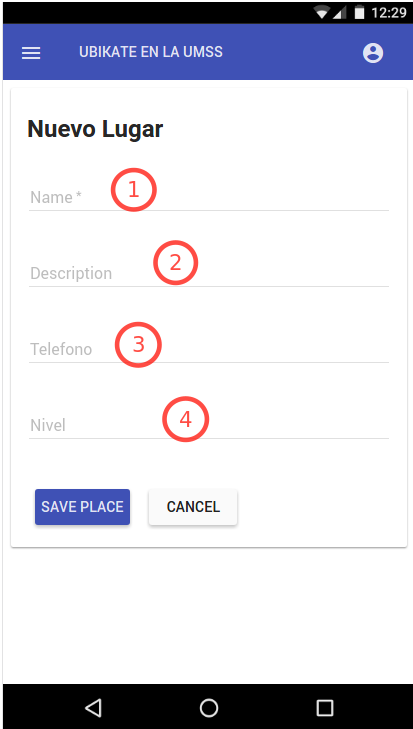
\includegraphics[width=0.3\textwidth]{manual_usuario/registro_place}

        \caption{Formulario de Registro de un Lugar.}
        \label{fig:vista_registro_place}
        \caption*{Fuente: Elaboración propia.}
      \end{center}
\end{figure}

\section{Información del Lugar}

La \emph{información de un lugar}, ver la figura \ref{fig:vista_información_lugar}, contiene los siguientes datos:
\begin{enumerate}
  \item La \emph{Foto} o imagen del lugar.
  \item La \emph{Información} del lugar, todos los datos ingresados en el \emph{formulario de registro}.
  \item El \emph{Botón para agregar imagenes} del lugar, las imágenes agregadas serán desplegadas en la parte superior de la \emph{información del lugar}.
  \item El \emph{Botón para encontrar la Ruta óptima al lugar}, al seleccionar esta opción se despliega el mapa del campus Universitario. Ver la figura \ref{fig:vista_ruta}.
  \item El \emph{Botón para Editar la Información del lugar}, al seleccionar esta opción se despliega el \emph{Formulario de edición de un Lugar}.
\end{enumerate}


\begin{figure}[H]
      \begin{center}
        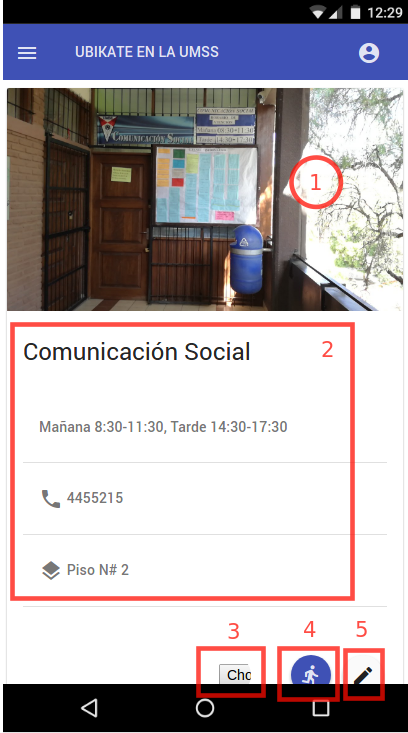
\includegraphics[width=0.25\textwidth]{manual_usuario/informacion_lugar}

        \caption{Información de un Lugar.}
        \label{fig:vista_información_lugar}
        \caption*{Fuente: Elaboración propia.}
      \end{center}
\end{figure}


\begin{figure}[H]
      \begin{center}
        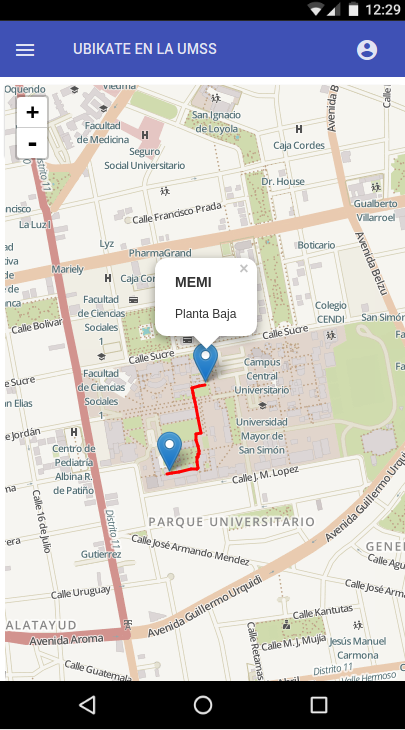
\includegraphics[width=0.25\textwidth]{manual_usuario/ruta}

        \caption{Vista del camino o ruta óptima al lugar.}
        \label{fig:vista_ruta}
        \caption*{Fuente: Elaboración propia.}
      \end{center}
\end{figure}


% \begin{figure}[H]
%   \centering
%   \begin{minipage}[b]{0.3\textwidth}
%     \includegraphics[width=\textwidth]{manual_usuario/información_lugar}
%     \caption{Información de un Lugar.}
%     \label{fig:vista_información_lugar}
%     % \caption*{Fuente: Elaboración propia.}
%   \end{minipage}
%   % \hfill
%   % \hspace*{3cm}
%   \blank{3cm}
%
%   \begin{minipage}[b]{0.3\textwidth}
%     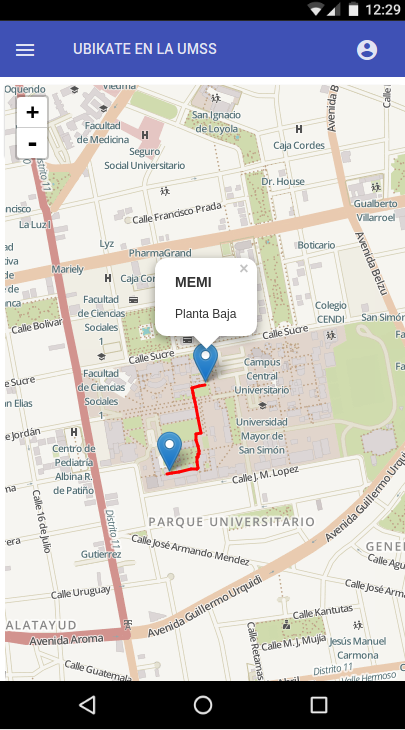
\includegraphics[width=\textwidth]{manual_usuario/ruta}
%     \caption{Vista del camino o ruta óptima al lugar.}
%     \label{fig:vista_ruta}
%     % \caption*{Fuente: Elaboración propia.}
%   \end{minipage}
%   \caption*{Fuente: Elaboración propia.}
%
% \end{figure}


\section{Formulario de edición de un Lugar}

El \emph{formulario de edición de un lugar} contiene la misma información que el \emph{formulario de registro de un lugar}, pero en el formulario de edición está desplegada la información del lugar para ser edita, ver la figura \ref{fig:vista_edicion_lugar}.

\begin{figure}[H]
      \begin{center}
        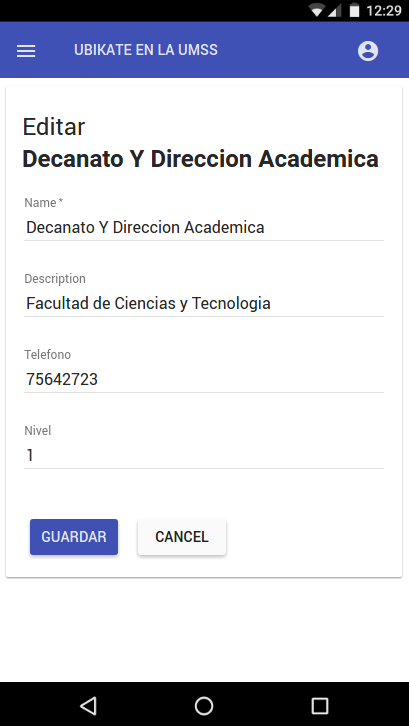
\includegraphics[width=0.25\textwidth]{manual_usuario/edicion}

        \caption{Formulario de edición de un lugar.}
        \label{fig:vista_edicion_lugar}
        \caption*{Fuente: Elaboración propia.}
      \end{center}
\end{figure}



\section{Formulario de registro de un Usuario}

Dentro del \emph{formulario de registro de un usuario} todos los campos son necesario, en caso de no ingresar un dato, la aplicación muestra un mensaje indicando que el campo es requerido. Como se puede ver en la figura \ref{fig:vista_registro_user}, dentro de este formulario se pueden ver los siguientes campos:
\begin{enumerate}
  \item El \emph{Nombre} del usuario.
  \item El \emph{Email} del usuario.
  \item La \emph{Razón} o el \emph{Porque} del registro.
\end{enumerate}

\begin{figure}[H]
      \begin{center}
        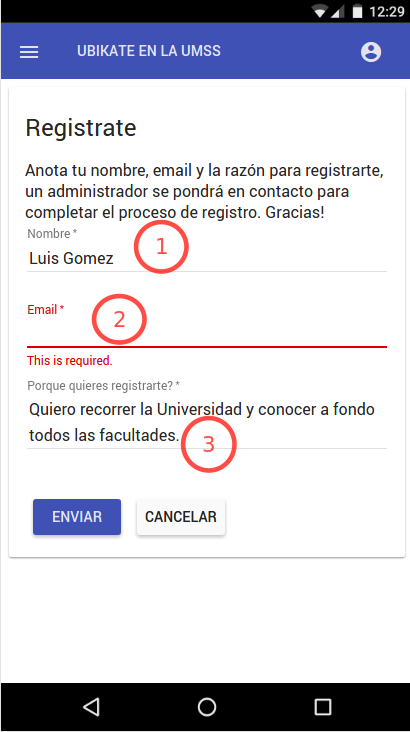
\includegraphics[width=0.25\textwidth]{manual_usuario/registro_usuario}

        \caption{Formulario de registro de un Usuario.}
        \label{fig:vista_registro_user}
        \caption*{Fuente: Elaboración propia.}
      \end{center}
\end{figure}


\section{Formulario de ingreso al sistema}

El \emph{formulario de ingreso al sistema} o \emph{Login}, ver figura \ref{fig:vista_login}, nos permite acceder al sistema con permisos de \emph{Administrador} o de \emph{Usuario Registrado}.

\begin{figure}[H]
      \begin{center}
        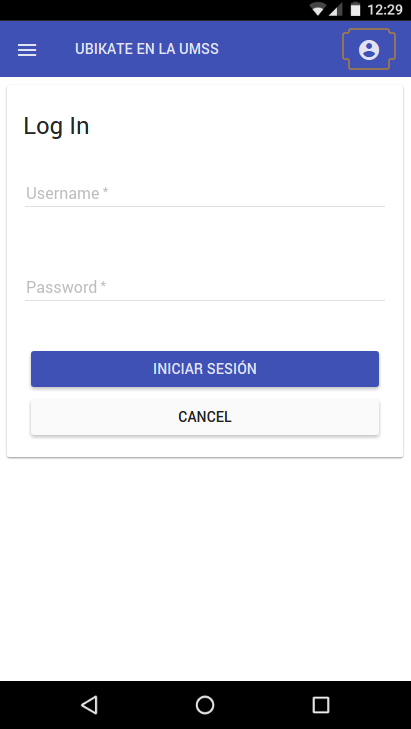
\includegraphics[width=0.25\textwidth]{manual_usuario/login}

        \caption{Formulario de ingreso al sistema.}
        \label{fig:vista_login}
        \caption*{Fuente: Elaboración propia.}
      \end{center}
\end{figure}


\section{Reporte}

El \emph{Reporte} mostrado en la figura \ref{fig:vista_reporte}, muestra los lugares más visitados por los usuarios de la aplicación, para acceder a él es necesario seleccionar la opción \emph{Reporte} del Menú.

\begin{figure}[H]
      \begin{center}
        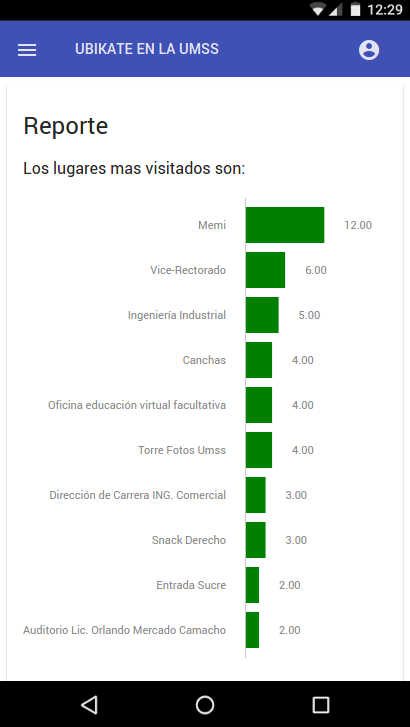
\includegraphics[width=0.25\textwidth]{manual_usuario/reporte}

        \caption{Lugares más visitados.}
        \label{fig:vista_reporte}
        \caption*{Fuente: Elaboración propia.}
      \end{center}
\end{figure}

  \end{appendices}

  \cleardoublepage
  \phantomsection
  \addcontentsline{toc}{part}{Índice de Figuras}
  \listoffigures

  \cleardoublepage
  \phantomsection
  \addcontentsline{toc}{part}{Índice de Tablas}
  \listoftables

\end{document}
